% =============================================================
% main.tex — Matemagica
% Documento principale LuaLaTeX
%
% COMPILAZIONE:
%   lualatex main.tex
%   lualatex main.tex   (secondo passaggio per riferimenti)
%
% STRUTTURA:
%   main.tex
%   preamble.tex          (pacchetti, font, colori, riquadri)
%   capitoli/
%     01.numeri.tex
%     02.operazioni_aritmetiche.tex
%     ...
%   immagini/
% =============================================================

\documentclass[
  a4paper,
  12pt,
  twoside,
  openright
]{book}

% ============================================================
%  preamble.tex — Matemagica
%  Da includere in main.tex con % ============================================================
%  preamble.tex — Matemagica
%  Da includere in main.tex con % ============================================================
%  preamble.tex — Matemagica
%  Da includere in main.tex con \input{preamble}
% ============================================================

% --- Compilatore -----------------------------------------------
% Richiede LuaLaTeX

% --- Pacchetti di base -----------------------------------------
\usepackage{fontspec}          % Gestione font OpenType (LuaLaTeX)
\usepackage{unicode-math}      % Matematica Unicode
\usepackage{microtype}         % Ottimizzazione tipografica
\microtypesetup{verbose=silent}
\usepackage{geometry}          % Impostazione pagina
\usepackage{setspace}          % Interlinea
\usepackage{parskip}           % Spaziatura tra paragrafi
\usepackage{ragged2e}          % Testo allineato a sinistra
\usepackage{xcolor}            % Colori
\usepackage{tcolorbox}         % Riquadri colorati
\tcbuselibrary{skins, breakable}
\usepackage{booktabs}          % Tabelle professionali
\usepackage{tikz}              % Disegni e diagrammi
\usetikzlibrary{decorations.pathreplacing}
\usepackage{amsmath}           % Matematica
\usepackage{enumitem}          % Liste personalizzate
\usepackage{hyperref}          % Link PDF

% --- Font ------------------------------------------------------
\setmainfont{Atkinson Hyperlegible}
\setmathfont{Latin Modern Math}

% --- Geometria pagina (A5) -------------------------------------
\geometry{
  paper      = a4paper,
  top        = 2.0cm,
  bottom     = 2.0cm,
  inner      = 2.2cm,   % margine interno leggermente più largo
  outer      = 1.8cm,
  marginpar  = 0cm,
}

% --- Tipografia ------------------------------------------------
\setstretch{1.5}              % Interlinea aumentata (accessibilità)
\RaggedRight                  % Testo allineato a sinistra (no giustificazione)
\setlength{\parindent}{0pt}   % Nessun rientro (già gestito da parskip)
\setlength{\parskip}{6pt}

% --- Palette colori --------------------------------------------
\definecolor{blu}{HTML}{2E6DA4}        % Primario — titoli, accenti
\definecolor{azzurro}{HTML}{D6EAF8}    % Secondario — riquadri definizioni
\definecolor{ambra}{HTML}{FEF9E7}      % Terziario — riquadri attenzione
\definecolor{ambraborder}{HTML}{F0C040}% Bordo ambra
\definecolor{lightgray}{HTML}{999999}      % Testi secondari (piè di pagina)
\definecolor{darkgray}{HTML}{666666}       % Sottotitolo

% --- Stili titoli di capitolo/sezione --------------------------
\usepackage{titlesec}
\usepackage{needspace}
\titleformat{\chapter}[block]
{\huge\bfseries\color{blu}}
{\thechapter.}{0.5em}{}
\titleformat{\section}[block]
{\large\bfseries\color{blu}}
{\thesection}{0.5em}{}
\titleformat{\subsection}[block]
{\normalsize\bfseries\color{blu}}
{\thesubsection}{0.5em}{}
\titlespacing*{\section}{0pt}{1.5ex plus 0.5ex minus 0.2ex}{0.8ex}
\titlespacing*{\subsection}{0pt}{1.2ex plus 0.4ex minus 0.2ex}{0.6ex}
\preto\section{\needspace{6\baselineskip}}
\preto\subsection{\needspace{5\baselineskip}}
\preto\subsubsection{\needspace{4\baselineskip}}

% --- Intestazione e piè di pagina -----------------------------
\usepackage{datetime2}         % Data di compilazione (LuaLaTeX-safe)
\usepackage{fancyhdr}

% Formato data AAAAMMDD — definito e attivato prima di \DTMtoday
\DTMnewdatestyle{aaaammdd}{%
  \renewcommand{\DTMdisplaydate}[4]{{\small\color{gray}ver. \number##1\DTMtwodigits{##2}\DTMtwodigits{##3}}}%
  \renewcommand{\DTMDisplaydate}{\DTMdisplaydate}%
}
\DTMsetdatestyle{aaaammdd}

\pagestyle{fancy}
\fancyhf{}                     % Azzera tutti i campi

% Piè di pagina: data sul lato interno, numero pagina sul lato esterno
% Pagine dispari (destra): data a sinistra (interno), numero a destra (esterno)
% Pagine pari  (sinistra): numero a sinistra (esterno), data a destra (interno)
\fancyfoot[LO]{\DTMtoday}
\fancyfoot[RO]{\thepage}
\fancyfoot[LE]{\thepage}
\fancyfoot[RE]{\DTMtoday}

\fancyhead{}                        % Nessuna intestazione
\renewcommand{\headrulewidth}{0pt}  % Nessuna riga sotto l'intestazione
\renewcommand{\footrulewidth}{0pt}  % Nessuna riga sopra il piè di pagina

% Stile plain — applicato automaticamente alla prima pagina di ogni capitolo
\fancypagestyle{plain}{
  \fancyhf{}
  \fancyfoot[LO]{\DTMtoday}
  \fancyfoot[RO]{\thepage}
  \fancyfoot[LE]{\thepage}
  \fancyfoot[RE]{\DTMtoday}
  \renewcommand{\headrulewidth}{0pt}
}

% --- Hyperref --------------------------------------------------
\hypersetup{
  colorlinks = true,
  linkcolor  = blu,
  urlcolor   = blu,
  pdftitle   = {Matemagica},
  pdfauthor  = {},
}

% ============================================================
%  stili/riquadri.tex — Ambienti riquadro
%  (può essere separato in un file a parte)
% ============================================================

% --- Riquadro DEFINIZIONE (azzurro) ----------------------------
\newtcolorbox{definizione}{
  enhanced,
  %  breakable,
  colback    = azzurro,
  colframe   = blu,
  fonttitle  = \bfseries,
  title      = Definizione,
  left       = 6pt,
  right      = 6pt,
  top        = 4pt,
  bottom     = 4pt,
  arc        = 4pt,
}

% --- Riquadro REGOLA (azzurro, bordo più sottile) ---------------
\newtcolorbox{regola}{
  enhanced,
  %  breakable,
  colback    = azzurro,
  colframe   = blu,
  fonttitle  = \bfseries,
  title      = Regola,
  left       = 6pt,
  right      = 6pt,
  top        = 4pt,
  bottom     = 4pt,
  arc        = 4pt,
}

% --- Riquadro ESEMPIO (bianco con bordo blu) --------------------
\newtcolorbox{esempio}{
  enhanced,
  breakable,
  colback    = white,
  colframe   = blu,
  fonttitle  = \bfseries,
  title      = Esempio,
  left       = 6pt,
  right      = 6pt,
  top        = 4pt,
  bottom     = 4pt,
  arc        = 4pt,
  boxrule    = 0.6pt,
}

% --- Riquadro ATTENZIONE (ambra) --------------------------------
\newtcolorbox{attenzione}{
  enhanced,
  breakable,
  colback    = ambra,
  colframe   = ambraborder,
  left       = 6pt,
  right      = 6pt,
  top        = 4pt,
  bottom     = 4pt,
  arc        = 4pt,
}

% --- Riquadro LO SAPEVI? (blu attenuato) ------------------------
\newtcolorbox{sapevi}{
  enhanced,
  breakable,
  colback    = blu!10,
  colframe   = blu!60,
  left       = 6pt,
  right      = 6pt,
  top        = 4pt,
  bottom     = 4pt,
  arc        = 4pt,
  fontupper  = \small,
}
% ============================================================

% --- Compilatore -----------------------------------------------
% Richiede LuaLaTeX

% --- Pacchetti di base -----------------------------------------
\usepackage{fontspec}          % Gestione font OpenType (LuaLaTeX)
\usepackage{unicode-math}      % Matematica Unicode
\usepackage{microtype}         % Ottimizzazione tipografica
\microtypesetup{verbose=silent}
\usepackage{geometry}          % Impostazione pagina
\usepackage{setspace}          % Interlinea
\usepackage{parskip}           % Spaziatura tra paragrafi
\usepackage{ragged2e}          % Testo allineato a sinistra
\usepackage{xcolor}            % Colori
\usepackage{tcolorbox}         % Riquadri colorati
\tcbuselibrary{skins, breakable}
\usepackage{booktabs}          % Tabelle professionali
\usepackage{tikz}              % Disegni e diagrammi
\usetikzlibrary{decorations.pathreplacing}
\usepackage{amsmath}           % Matematica
\usepackage{enumitem}          % Liste personalizzate
\usepackage{hyperref}          % Link PDF

% --- Font ------------------------------------------------------
\setmainfont{Atkinson Hyperlegible}
\setmathfont{Latin Modern Math}

% --- Geometria pagina (A5) -------------------------------------
\geometry{
  paper      = a4paper,
  top        = 2.0cm,
  bottom     = 2.0cm,
  inner      = 2.2cm,   % margine interno leggermente più largo
  outer      = 1.8cm,
  marginpar  = 0cm,
}

% --- Tipografia ------------------------------------------------
\setstretch{1.5}              % Interlinea aumentata (accessibilità)
\RaggedRight                  % Testo allineato a sinistra (no giustificazione)
\setlength{\parindent}{0pt}   % Nessun rientro (già gestito da parskip)
\setlength{\parskip}{6pt}

% --- Palette colori --------------------------------------------
\definecolor{blu}{HTML}{2E6DA4}        % Primario — titoli, accenti
\definecolor{azzurro}{HTML}{D6EAF8}    % Secondario — riquadri definizioni
\definecolor{ambra}{HTML}{FEF9E7}      % Terziario — riquadri attenzione
\definecolor{ambraborder}{HTML}{F0C040}% Bordo ambra
\definecolor{lightgray}{HTML}{999999}      % Testi secondari (piè di pagina)
\definecolor{darkgray}{HTML}{666666}       % Sottotitolo

% --- Stili titoli di capitolo/sezione --------------------------
\usepackage{titlesec}
\usepackage{needspace}
\titleformat{\chapter}[block]
{\huge\bfseries\color{blu}}
{\thechapter.}{0.5em}{}
\titleformat{\section}[block]
{\large\bfseries\color{blu}}
{\thesection}{0.5em}{}
\titleformat{\subsection}[block]
{\normalsize\bfseries\color{blu}}
{\thesubsection}{0.5em}{}
\titlespacing*{\section}{0pt}{1.5ex plus 0.5ex minus 0.2ex}{0.8ex}
\titlespacing*{\subsection}{0pt}{1.2ex plus 0.4ex minus 0.2ex}{0.6ex}
\preto\section{\needspace{6\baselineskip}}
\preto\subsection{\needspace{5\baselineskip}}
\preto\subsubsection{\needspace{4\baselineskip}}

% --- Intestazione e piè di pagina -----------------------------
\usepackage{datetime2}         % Data di compilazione (LuaLaTeX-safe)
\usepackage{fancyhdr}

% Formato data AAAAMMDD — definito e attivato prima di \DTMtoday
\DTMnewdatestyle{aaaammdd}{%
  \renewcommand{\DTMdisplaydate}[4]{{\small\color{gray}ver. \number##1\DTMtwodigits{##2}\DTMtwodigits{##3}}}%
  \renewcommand{\DTMDisplaydate}{\DTMdisplaydate}%
}
\DTMsetdatestyle{aaaammdd}

\pagestyle{fancy}
\fancyhf{}                     % Azzera tutti i campi

% Piè di pagina: data sul lato interno, numero pagina sul lato esterno
% Pagine dispari (destra): data a sinistra (interno), numero a destra (esterno)
% Pagine pari  (sinistra): numero a sinistra (esterno), data a destra (interno)
\fancyfoot[LO]{\DTMtoday}
\fancyfoot[RO]{\thepage}
\fancyfoot[LE]{\thepage}
\fancyfoot[RE]{\DTMtoday}

\fancyhead{}                        % Nessuna intestazione
\renewcommand{\headrulewidth}{0pt}  % Nessuna riga sotto l'intestazione
\renewcommand{\footrulewidth}{0pt}  % Nessuna riga sopra il piè di pagina

% Stile plain — applicato automaticamente alla prima pagina di ogni capitolo
\fancypagestyle{plain}{
  \fancyhf{}
  \fancyfoot[LO]{\DTMtoday}
  \fancyfoot[RO]{\thepage}
  \fancyfoot[LE]{\thepage}
  \fancyfoot[RE]{\DTMtoday}
  \renewcommand{\headrulewidth}{0pt}
}

% --- Hyperref --------------------------------------------------
\hypersetup{
  colorlinks = true,
  linkcolor  = blu,
  urlcolor   = blu,
  pdftitle   = {Matemagica},
  pdfauthor  = {},
}

% ============================================================
%  stili/riquadri.tex — Ambienti riquadro
%  (può essere separato in un file a parte)
% ============================================================

% --- Riquadro DEFINIZIONE (azzurro) ----------------------------
\newtcolorbox{definizione}{
  enhanced,
  %  breakable,
  colback    = azzurro,
  colframe   = blu,
  fonttitle  = \bfseries,
  title      = Definizione,
  left       = 6pt,
  right      = 6pt,
  top        = 4pt,
  bottom     = 4pt,
  arc        = 4pt,
}

% --- Riquadro REGOLA (azzurro, bordo più sottile) ---------------
\newtcolorbox{regola}{
  enhanced,
  %  breakable,
  colback    = azzurro,
  colframe   = blu,
  fonttitle  = \bfseries,
  title      = Regola,
  left       = 6pt,
  right      = 6pt,
  top        = 4pt,
  bottom     = 4pt,
  arc        = 4pt,
}

% --- Riquadro ESEMPIO (bianco con bordo blu) --------------------
\newtcolorbox{esempio}{
  enhanced,
  breakable,
  colback    = white,
  colframe   = blu,
  fonttitle  = \bfseries,
  title      = Esempio,
  left       = 6pt,
  right      = 6pt,
  top        = 4pt,
  bottom     = 4pt,
  arc        = 4pt,
  boxrule    = 0.6pt,
}

% --- Riquadro ATTENZIONE (ambra) --------------------------------
\newtcolorbox{attenzione}{
  enhanced,
  breakable,
  colback    = ambra,
  colframe   = ambraborder,
  left       = 6pt,
  right      = 6pt,
  top        = 4pt,
  bottom     = 4pt,
  arc        = 4pt,
}

% --- Riquadro LO SAPEVI? (blu attenuato) ------------------------
\newtcolorbox{sapevi}{
  enhanced,
  breakable,
  colback    = blu!10,
  colframe   = blu!60,
  left       = 6pt,
  right      = 6pt,
  top        = 4pt,
  bottom     = 4pt,
  arc        = 4pt,
  fontupper  = \small,
}
% ============================================================

% --- Compilatore -----------------------------------------------
% Richiede LuaLaTeX

% --- Pacchetti di base -----------------------------------------
\usepackage{fontspec}          % Gestione font OpenType (LuaLaTeX)
\usepackage{unicode-math}      % Matematica Unicode
\usepackage{microtype}         % Ottimizzazione tipografica
\microtypesetup{verbose=silent}
\usepackage{geometry}          % Impostazione pagina
\usepackage{setspace}          % Interlinea
\usepackage{parskip}           % Spaziatura tra paragrafi
\usepackage{ragged2e}          % Testo allineato a sinistra
\usepackage{xcolor}            % Colori
\usepackage{tcolorbox}         % Riquadri colorati
\tcbuselibrary{skins, breakable}
\usepackage{booktabs}          % Tabelle professionali
\usepackage{tikz}              % Disegni e diagrammi
\usetikzlibrary{decorations.pathreplacing}
\usepackage{amsmath}           % Matematica
\usepackage{enumitem}          % Liste personalizzate
\usepackage{hyperref}          % Link PDF

% --- Font ------------------------------------------------------
\setmainfont{Atkinson Hyperlegible}
\setmathfont{Latin Modern Math}

% --- Geometria pagina (A5) -------------------------------------
\geometry{
  paper      = a4paper,
  top        = 2.0cm,
  bottom     = 2.0cm,
  inner      = 2.2cm,   % margine interno leggermente più largo
  outer      = 1.8cm,
  marginpar  = 0cm,
}

% --- Tipografia ------------------------------------------------
\setstretch{1.5}              % Interlinea aumentata (accessibilità)
\RaggedRight                  % Testo allineato a sinistra (no giustificazione)
\setlength{\parindent}{0pt}   % Nessun rientro (già gestito da parskip)
\setlength{\parskip}{6pt}

% --- Palette colori --------------------------------------------
\definecolor{blu}{HTML}{2E6DA4}        % Primario — titoli, accenti
\definecolor{azzurro}{HTML}{D6EAF8}    % Secondario — riquadri definizioni
\definecolor{ambra}{HTML}{FEF9E7}      % Terziario — riquadri attenzione
\definecolor{ambraborder}{HTML}{F0C040}% Bordo ambra
\definecolor{lightgray}{HTML}{999999}      % Testi secondari (piè di pagina)
\definecolor{darkgray}{HTML}{666666}       % Sottotitolo

% --- Stili titoli di capitolo/sezione --------------------------
\usepackage{titlesec}
\usepackage{needspace}
\titleformat{\chapter}[block]
{\huge\bfseries\color{blu}}
{\thechapter.}{0.5em}{}
\titleformat{\section}[block]
{\large\bfseries\color{blu}}
{\thesection}{0.5em}{}
\titleformat{\subsection}[block]
{\normalsize\bfseries\color{blu}}
{\thesubsection}{0.5em}{}
\titlespacing*{\section}{0pt}{1.5ex plus 0.5ex minus 0.2ex}{0.8ex}
\titlespacing*{\subsection}{0pt}{1.2ex plus 0.4ex minus 0.2ex}{0.6ex}
\preto\section{\needspace{6\baselineskip}}
\preto\subsection{\needspace{5\baselineskip}}
\preto\subsubsection{\needspace{4\baselineskip}}

% --- Intestazione e piè di pagina -----------------------------
\usepackage{datetime2}         % Data di compilazione (LuaLaTeX-safe)
\usepackage{fancyhdr}

% Formato data AAAAMMDD — definito e attivato prima di \DTMtoday
\DTMnewdatestyle{aaaammdd}{%
  \renewcommand{\DTMdisplaydate}[4]{{\small\color{gray}ver. \number##1\DTMtwodigits{##2}\DTMtwodigits{##3}}}%
  \renewcommand{\DTMDisplaydate}{\DTMdisplaydate}%
}
\DTMsetdatestyle{aaaammdd}

\pagestyle{fancy}
\fancyhf{}                     % Azzera tutti i campi

% Piè di pagina: data sul lato interno, numero pagina sul lato esterno
% Pagine dispari (destra): data a sinistra (interno), numero a destra (esterno)
% Pagine pari  (sinistra): numero a sinistra (esterno), data a destra (interno)
\fancyfoot[LO]{\DTMtoday}
\fancyfoot[RO]{\thepage}
\fancyfoot[LE]{\thepage}
\fancyfoot[RE]{\DTMtoday}

\fancyhead{}                        % Nessuna intestazione
\renewcommand{\headrulewidth}{0pt}  % Nessuna riga sotto l'intestazione
\renewcommand{\footrulewidth}{0pt}  % Nessuna riga sopra il piè di pagina

% Stile plain — applicato automaticamente alla prima pagina di ogni capitolo
\fancypagestyle{plain}{
  \fancyhf{}
  \fancyfoot[LO]{\DTMtoday}
  \fancyfoot[RO]{\thepage}
  \fancyfoot[LE]{\thepage}
  \fancyfoot[RE]{\DTMtoday}
  \renewcommand{\headrulewidth}{0pt}
}

% --- Hyperref --------------------------------------------------
\hypersetup{
  colorlinks = true,
  linkcolor  = blu,
  urlcolor   = blu,
  pdftitle   = {Matemagica},
  pdfauthor  = {},
}

% ============================================================
%  stili/riquadri.tex — Ambienti riquadro
%  (può essere separato in un file a parte)
% ============================================================

% --- Riquadro DEFINIZIONE (azzurro) ----------------------------
\newtcolorbox{definizione}{
  enhanced,
  %  breakable,
  colback    = azzurro,
  colframe   = blu,
  fonttitle  = \bfseries,
  title      = Definizione,
  left       = 6pt,
  right      = 6pt,
  top        = 4pt,
  bottom     = 4pt,
  arc        = 4pt,
}

% --- Riquadro REGOLA (azzurro, bordo più sottile) ---------------
\newtcolorbox{regola}{
  enhanced,
  %  breakable,
  colback    = azzurro,
  colframe   = blu,
  fonttitle  = \bfseries,
  title      = Regola,
  left       = 6pt,
  right      = 6pt,
  top        = 4pt,
  bottom     = 4pt,
  arc        = 4pt,
}

% --- Riquadro ESEMPIO (bianco con bordo blu) --------------------
\newtcolorbox{esempio}{
  enhanced,
  breakable,
  colback    = white,
  colframe   = blu,
  fonttitle  = \bfseries,
  title      = Esempio,
  left       = 6pt,
  right      = 6pt,
  top        = 4pt,
  bottom     = 4pt,
  arc        = 4pt,
  boxrule    = 0.6pt,
}

% --- Riquadro ATTENZIONE (ambra) --------------------------------
\newtcolorbox{attenzione}{
  enhanced,
  breakable,
  colback    = ambra,
  colframe   = ambraborder,
  left       = 6pt,
  right      = 6pt,
  top        = 4pt,
  bottom     = 4pt,
  arc        = 4pt,
}

% --- Riquadro LO SAPEVI? (blu attenuato) ------------------------
\newtcolorbox{sapevi}{
  enhanced,
  breakable,
  colback    = blu!10,
  colframe   = blu!60,
  left       = 6pt,
  right      = 6pt,
  top        = 4pt,
  bottom     = 4pt,
  arc        = 4pt,
  fontupper  = \small,
}

% =============================================================
\begin{document}
% =============================================================

% -------------------------------------------------------------
% FRONTESPIZIO
% -------------------------------------------------------------
\begin{titlepage}
  \centering
  \vspace*{3cm}

  {\color{blu}\rule{\linewidth}{1.5pt}}
  \vspace{0.6cm}

  {\Huge\bfseries\color{blu} Matemagica}\\[0.4cm]
  {\color{black}Libro di supporto per l'apprendimento della matematica nelle scuole medie}\\[0.2cm]
  {\small\color{darkgray} Ispirato al Piano di studio DECS, Canton Ticino, Svizzera}

  \vspace{0.6cm}
  {\color{blu}\rule{\linewidth}{1.5pt}}

  \vfill

  \vspace{2cm}
  {\small\color{black}Francesco ed Emma Piraneo Giuliano, \the\year}
\end{titlepage}

% -------------------------------------------------------------
% PAGINE PRELIMINARI
% -------------------------------------------------------------
\frontmatter
\tableofcontents
\clearpage

% -------------------------------------------------------------
% CORPO DEL LIBRO
% -------------------------------------------------------------
\mainmatter

% ============================================================
%  colophon.tex — Matemagica
%  Da includere in main.tex prima di \end{document}
%  Uso: \input{colophon}
% ============================================================

\cleardoublepage
\thispagestyle{empty}

\vspace*{\fill}

{\small
    \begin{center}
        {\large\bfseries\color{blu} Matemagica}\\[4pt]
        {\normalsize Libro di supporto per l'apprendimento della matematica nelle scuole medie}\\[2pt]
        {\normalsize Ispirato al Piano di studio DECS, Canton Ticino}
    \end{center}

    \medskip
    \noindent\rule{\linewidth}{0.4pt}
    \medskip

    \noindent\textbf{Autore:} Francesco ed Emma Piraneo G.\\
    \textbf{Composizione e ottimizzazione:} Claude Sonnet\\
    \textbf{Lingua:} Italiano\\
    \textbf{Fascia scolastica:} Scuola media, anni 1–4 (età 11–14 anni)\\
    \textbf{Formato:} A4, ottimizzato per stampa e lettura digitale (PDF)\\
    \textbf{Composizione:} LuaLaTeX\\
    \textbf{Font testo:} Atkinson Hyperlegible — Braille Institute of America\\
    \textbf{Font matematica:} Latin Modern Math\\
    \textbf{Repository:} \href{https://github.com/fpiraneo/matemagica}{\texttt{github.com/fpiraneo/matemagica}}

    \medskip
    \noindent\rule{\linewidth}{0.4pt}
    \medskip

    \noindent\textbf{Licenza d'uso}

    \smallskip
    \noindent Quest'opera è distribuita con licenza\\
    \textbf{Creative Commons Attribuzione – Non Commerciale –}\\
    \textbf{Condividi allo stesso modo 4.0 Internazionale (CC BY-NC-SA 4.0).}

    \smallskip
    \noindent\href{https://creativecommons.org/licenses/by-nc-sa/4.0/deed.it}%
    {\texttt{creativecommons.org/licenses/by-nc-sa/4.0/deed.it}}

    \medskip

    \noindent\textbf{È vietato qualsiasi uso commerciale} di questo materiale, anche parziale.
    Ogni riproduzione o adattamento — anche parziale — deve includere
    un'attribuzione esplicita all'autore e alla fonte originale.

    \medskip

    \noindent Formula di attribuzione richiesta:

    \smallskip
    \begin{center}
        \textit{«Matemagica\\
            di Francesco ed Emma Piraneo Giuliano.\\
            Distribuito con licenza CC BY-NC-SA 4.0.\\
            Fonte: \href{https://github.com/fpiraneo/matemagica}{\texttt{github.com/fpiraneo/matemagica}}»}
    \end{center}

    \medskip
    \noindent\rule{\linewidth}{0.4pt}
    \medskip

    \noindent\textbf{Avvertenze}

    \smallskip
    \noindent I contenuti sono stati redatti con cura ispirandosi al Piano di studio DECS,
    ma non garantiscono completezza o aggiornamento rispetto a versioni successive
    del curricolo ufficiale. Il materiale è fornito \textit{«così com'è»}, senza garanzie
    di alcun tipo. L'autore declina ogni responsabilità per eventuali errori od omissioni.

    \smallskip
    \noindent Questo progetto non ha alcun endorsement ufficiale da parte del DECS,
    del Canton Ticino o di qualsiasi istituzione scolastica.
    Il materiale non sostituisce l'insegnamento frontale di un docente qualificato.

    \medskip
    \noindent\rule{\linewidth}{0.4pt}
    \medskip

    \begin{center}
        {\footnotesize Copyright \textcopyright\ Francesco ed Emma Piraneo Giuliano, \the\year.\\
            Tutti i diritti non espressamente concessi sono riservati.}
    \end{center}

} % fine \small

\vspace*{\fill}
% ============================================================
%  Capitolo 1 — I numeri
%  Matemagica — Libro di matematica per le scuole medie
%  Canton Ticino (DECS)
% ============================================================

\chapter{I numeri}

% ------------------------------------------------------------
\section*{Obiettivi di apprendimento}
% ------------------------------------------------------------

Al termine di questo capitolo l'allievo sarà in grado di:

\begin{itemize}
  \item Spiegare cosa sono i numeri e a cosa servono.
  \item Riconoscere e utilizzare le \textbf{cifre arabe} nel sistema di numerazione decimale.
  \item Leggere e scrivere semplici numeri con la \textbf{numerazione romana}.
  \item Identificare e collocare i \textbf{numeri naturali} sulla retta numerica.
  \item Comprendere il \textbf{sistema posizionale decimale}.
  \item Utilizzare correttamente i \textbf{simboli di confronto} tra numeri.
\end{itemize}

\bigskip

% ============================================================
\section{Cosa sono i numeri}
% ============================================================

L'idea di numero è una delle conquiste intellettuali più antiche dell'umanità.
Risale ad almeno 300\,000 anni fa, quando gli esseri umani vivevano nelle caverne
e dedicavano quasi tutte le proprie energie alla ricerca del cibo.
In quell'epoca non era ancora nota la capacità di contare:
l'idea di quantità era limitata ai piccoli insiemi che si potevano riconoscere
a colpo d'occhio — 1, 2, 3 e 4 oggetti.
Per quantità maggiori si ricorreva a espressioni generiche
come \emph{mucchio}, \emph{molti} o \emph{tanti}.

\medskip

Nel corso dei secoli, le civiltà hanno elaborato modalità diverse
per rappresentare i numeri, ciascuna con caratteristiche proprie.

\begin{definizione}
  Un \textbf{numero} è un insieme di simboli, chiamati \textbf{cifre},
  che indica una quantità.
\end{definizione}

% ------------------------------------------------------------
\subsection{Il sistema di numerazione arabo}
% ------------------------------------------------------------

Il sistema di numerazione che utilizziamo ogni giorno fu sviluppato
dalle popolazioni dell'\textbf{India} e successivamente diffuso in Europa
dagli \textbf{Arabi}.
Per questo motivo le nostre cifre sono chiamate \textbf{cifre arabe}
o \textbf{cifre indo-arabiche}.

\begin{regola}
  Il sistema arabo utilizza esattamente \textbf{dieci cifre}:
  \[
    0,\quad 1,\quad 2,\quad 3,\quad 4,\quad 5,\quad 6,\quad 7,\quad 8,\quad 9
  \]
  Con queste dieci cifre è possibile scrivere qualsiasi numero.
\end{regola}

\begin{esempio}
  Con le sole cifre $3$, $0$ e $7$ possiamo formare, tra gli altri,
  i numeri $307$, $370$, $703$ e $730$.
  Ogni combinazione rappresenta una quantità diversa.
\end{esempio}

% ------------------------------------------------------------
\subsection{Cenni di numerazione romana}
% ------------------------------------------------------------

Un altro sistema di numerazione importante nella storia è quello \textbf{romano},
usato nell'antica Roma e ancora oggi presente su orologi, monumenti e capitoli dei libri.

\begin{regola}
  La numerazione romana utilizza sette \textbf{simboli} fondamentali:

  \medskip
  \begin{center}
    \begin{tabular}{cc}
      \toprule
      \textbf{Simbolo} & \textbf{Valore} \\
      \midrule
      I   &   1 \\
      V   &   5 \\
      X   &  10 \\
      L   &  50 \\
      C   & 100 \\
      D   & 500 \\
      M   & 1000 \\
      \bottomrule
    \end{tabular}
  \end{center}

  \medskip
  I simboli si \textbf{sommano} se un simbolo di valore minore segue uno di valore maggiore
  (es.\ $\mathrm{VI} = 6$);
  si \textbf{sottraggono} se un simbolo di valore minore precede uno di valore maggiore
  (es.\ $\mathrm{IV} = 4$).
\end{regola}

\begin{esempio}
  \[
    \mathrm{VIII} = 8 \qquad
    \mathrm{XIV} = 14 \qquad
    \mathrm{XL} = 40 \qquad
    \mathrm{MMXXVI} = 2026
  \]
\end{esempio}

\begin{attenzione}
  \textbf{Errore comune — numerazione romana:}
  non è consentito ripetere lo stesso simbolo più di tre volte di fila.
  Quindi $40$ non si scrive $\mathrm{XXXX}$, ma $\mathrm{XL}$.
\end{attenzione}

\begin{sapevi}
  \textbf{Lo sapevi?}
  Il sistema romano non possiede un simbolo per lo zero.
  Questa mancanza rese i calcoli molto complessi.
  L'introduzione dello \textbf{zero} come cifra vera e propria,
  avvenuta in India attorno al V secolo d.C.,
  fu una delle rivoluzioni matematiche più importanti della storia.
\end{sapevi}

% ============================================================
\section{I numeri naturali}
% ============================================================

I numeri che fin dalle origini l'essere umano ha usato per \textbf{contare}
oggetti, animali, persone e giorni prendono il nome di \textbf{numeri naturali}.

\begin{definizione}
  I \textbf{numeri naturali} sono i numeri interi non negativi utilizzati per contare.
  Si indicano con il simbolo $\mathbb{N}$:
  \[
    \mathbb{N} = \{0,\; 1,\; 2,\; 3,\; 4,\; 5,\; \ldots\}
  \]
  I puntini ($\ldots$) indicano che la sequenza continua all'infinito.
\end{definizione}

% ------------------------------------------------------------
\subsection{La retta numerica}
% ------------------------------------------------------------

I numeri naturali possono essere rappresentati graficamente su una
\textbf{retta numerica}: una semiretta orientata su cui i numeri
sono collocati a distanze uguali tra loro.

\medskip

\begin{center}
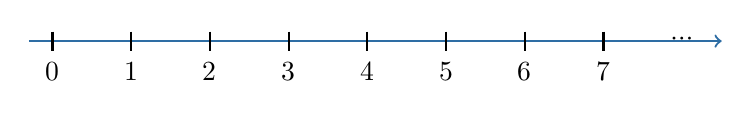
\begin{tikzpicture}
  % Retta
  \draw[->, thick, color=blu] (-0.3,0) -- (8.5,0);
  % Tacche e numeri
  \foreach \x/\n in {0/0, 1/1, 2/2, 3/3, 4/4, 5/5, 6/6, 7/7} {
    \draw[thick] (\x,0.12) -- (\x,-0.12);
    \node[below=4pt] at (\x,0) {$\n$};
  }
  % Puntini
  \node at (8,0) {$\cdots$};
\end{tikzpicture}
\end{center}

\begin{regola}
  Sulla retta numerica:
  \begin{itemize}
    \item L'\textbf{origine} corrisponde al numero $0$.
    \item Procedendo verso destra, i numeri \textbf{aumentano}.
    \item Ogni numero naturale $n$ possiede un \textbf{successivo} $n + 1$
          e, ad eccezione dello zero, un \textbf{precedente} $n - 1$.
    \item Tra un numero e il suo successivo non esiste alcun altro numero naturale.
  \end{itemize}
\end{regola}

\begin{attenzione}
  \textbf{Attenzione — i numeri naturali sono infiniti:}
  non esiste un numero naturale più grande di tutti gli altri.
  Per indicare questo fatto si scrivono i puntini ($\ldots$)
  all'estremità destra della sequenza.
\end{attenzione}

% ============================================================
\section{Il sistema posizionale decimale}
% ============================================================

Il modo di rappresentare i numeri che utilizziamo abitualmente
si chiama \textbf{sistema posizionale decimale}.

\begin{definizione}
  Nel \textbf{sistema posizionale decimale}:
  \begin{itemize}
    \item Si utilizzano \textbf{dieci cifre}: $0, 1, 2, 3, 4, 5, 6, 7, 8, 9$.
    \item Il \textbf{valore} di ciascuna cifra dipende dalla
          \textbf{posizione} che occupa nel numero.
  \end{itemize}
\end{definizione}

\begin{esempio}
  Nel numero $\mathbf{352}$:
  \begin{itemize}
    \item la cifra $3$ si trova nella posizione delle \textbf{centinaia}
          e vale $3 \times 100 = 300$;
    \item la cifra $5$ si trova nella posizione delle \textbf{decine}
          e vale $5 \times 10 = 50$;
    \item la cifra $2$ si trova nella posizione delle \textbf{unità}
          e vale $2 \times 1 = 2$.
  \end{itemize}
  Quindi: $352 = 300 + 50 + 2$.
\end{esempio}

\begin{attenzione}
  \textbf{Errore comune — il ruolo dello zero:}
  la cifra $0$ non indica «nulla da scrivere» ma occupa una posizione precisa.
  Nel numero $305$, lo zero occupa la posizione delle decine
  e indica che non ci sono decine: $305 = 300 + 0 + 5$.
  Senza lo zero, $305$ e $35$ sarebbero indistinguibili.
\end{attenzione}

\begin{sapevi}
  \textbf{Lo sapevi?}
  Il termine \textbf{decimale} deriva dal latino \emph{decem}, che significa dieci.
  La scelta di dieci come base del sistema è probabilmente legata
  al fatto che l'essere umano possiede dieci dita,
  che in tempi antichi erano il primo strumento di calcolo.
\end{sapevi}

% ============================================================
\section{Simboli di confronto}
% ============================================================

In matematica si usano simboli specifici per confrontare due numeri
ed esprimere la loro relazione.

\begin{definizione}
  I \textbf{simboli di confronto} (o \textbf{simboli di relazione})
  indicano la relazione di ordine tra due numeri o espressioni.
\end{definizione}

\begin{regola}
  I simboli di confronto fondamentali sono:

  \medskip
  \begin{center}
    \begin{tabular}{cll}
      \toprule
      \textbf{Simbolo} & \textbf{Nome} & \textbf{Esempio} \\
      \midrule
      $>$   & maggiore di          & $7 > 3$ \quad (7 è maggiore di 3) \\
      $<$   & minore di            & $3 < 7$ \quad (3 è minore di 7) \\
      $\geq$ & maggiore o uguale a & $5 \geq 5$ \quad (5 è maggiore o uguale a 5) \\
      $\leq$ & minore o uguale a   & $4 \leq 6$ \quad (4 è minore o uguale a 6) \\
      $=$   & uguale a             & $2 + 3 = 5$ \\
      $\neq$ & diverso da          & $4 \neq 7$ \quad (4 è diverso da 7) \\
      \bottomrule
    \end{tabular}
  \end{center}
\end{regola}

\begin{esempio}
  \textbf{Uso dei simboli di confronto — passo per passo.}

  \medskip
  \textit{Confrontare $48$ e $52$.}

  \begin{enumerate}
    \item Osserviamo le cifre delle \textbf{decine}: $48$ ha la cifra $4$,
          mentre $52$ ha la cifra $5$.
    \item Poiché $4 < 5$, il numero $48$ è minore di $52$.
    \item Scriviamo: \quad $48 < 52$.
  \end{enumerate}
\end{esempio}

\begin{esempio}
  \textit{Verificare se $6 + 4 \neq 11$.}

  \begin{enumerate}
    \item Calcoliamo il primo membro: $6 + 4 = 10$.
    \item Confrontiamo con $11$: $10 \neq 11$ è \textbf{vero}.
  \end{enumerate}
\end{esempio}

\begin{attenzione}
  \textbf{Errore comune — direzione del simbolo:}
  il simbolo \emph{apre} sempre verso il numero maggiore.
  $5 > 3$ e $3 < 5$ esprimono la stessa relazione vista da due direzioni diverse.
  Un metodo utile: immaginare il simbolo come una freccia che punta
  verso il numero più piccolo.
\end{attenzione}

\begin{sapevi}
  \textbf{Lo sapevi?}
  I simboli $<$ e $>$ furono introdotti dal matematico inglese
  \textbf{Thomas Harriot} nel 1631, nell'opera \emph{Artis Analyticae Praxis}.
  Prima di allora, i matematici esprimevano le relazioni di ordine
  soltanto a parole.
\end{sapevi}

% ============================================================
\section*{Riepilogo del capitolo}
% ============================================================

\begin{itemize}
  \item Un \textbf{numero} è un insieme di simboli (cifre) che indica una quantità.
  \item Il \textbf{sistema arabo} usa dieci cifre ($0$–$9$);
        il \textbf{sistema romano} usa sette simboli ($\mathrm{I, V, X, L, C, D, M}$).
  \item I \textbf{numeri naturali} ($\mathbb{N} = \{0, 1, 2, 3, \ldots\}$)
        servono a contare; sono infiniti e si rappresentano sulla retta numerica.
  \item Nel \textbf{sistema posizionale decimale} il valore di una cifra
        dipende dalla posizione che occupa nel numero.
  \item I \textbf{simboli di confronto}
        ($>, <, \geq, \leq, =, \neq$)
        esprimono la relazione tra due quantità.
\end{itemize}

% ============================================================
%  capitoli/operazioni_aritmetiche.tex — Matemagica
%  Le operazioni aritmetiche basilari e le loro proprietà
% ============================================================

\chapter{Operazioni aritmetiche --- Proprietà}

% --- Obiettivi di apprendimento --------------------------------
\section*{Obiettivi di apprendimento}
\begin{itemize}
  \item Conoscere le quattro operazioni aritmetiche basilari: addizione, sottrazione, moltiplicazione e divisione.
  \item Saper applicare correttamente le proprietà di ciascuna operazione.
  \item Riconoscere e prevenire gli errori più comuni nel calcolo.
  \item Comprendere la precedenza tra le operazioni.
\end{itemize}

\bigskip

% ============================================================
%  SEZIONE 1 — ADDIZIONE
% ============================================================
\section{L'addizione}

\begin{definizione}
  L'\textbf{addizione} è l'operazione che combina due o più numeri, detti \textbf{addendi}, per ottenere un unico numero chiamato \textbf{somma}.

  \[
    a + b = s
  \]

  dove $a$ e $b$ sono gli addendi e $s$ è la somma.
\end{definizione}

\subsection{Proprietà dell'addizione}

\begin{regola}
  \textbf{Proprietà commutativa}

  L'ordine degli addendi non cambia la somma:
  \[
    a + b = b + a
  \]
\end{regola}

\begin{esempio}
  \[
    3 + 7 = 7 + 3 = 10
  \]
  Cambiare l'ordine degli addendi non modifica il risultato.
\end{esempio}

\begin{regola}
  \textbf{Proprietà associativa}

  Quando si sommano tre o più addendi, il risultato non cambia raggruppandoli in modo diverso:
  \[
    (a + b) + c = a + (b + c)
  \]
\end{regola}

\begin{esempio}
  \[
    (2 + 5) + 3 = 7 + 3 = 10
  \]
  \[
    2 + (5 + 3) = 2 + 8 = 10
  \]
  Il risultato è lo stesso indipendentemente da come si raggruppano gli addendi.
\end{esempio}

\begin{regola}
  \textbf{Proprietà dell'elemento neutro}

  Aggiungere zero a qualsiasi numero lascia il numero invariato:
  \[
    a + 0 = 0 + a = a
  \]
  Lo \textbf{zero} è l'\textbf{elemento neutro} dell'addizione.
\end{regola}

\begin{esempio}
  \[
    15 + 0 = 15 \qquad \qquad 0 + 8 = 8
  \]
\end{esempio}

% ============================================================
%  SEZIONE 2 — SOTTRAZIONE
% ============================================================
\section{La sottrazione}

\begin{definizione}
  La \textbf{sottrazione} è l'operazione che, dati due numeri, calcola la loro \textbf{differenza}. Il primo numero si chiama \textbf{minuendo}, il secondo \textbf{sottraendo}.

  \[
    a - b = d
  \]

  dove $a$ è il minuendo, $b$ è il sottraendo e $d$ è la differenza.
\end{definizione}

\subsection{Proprietà della sottrazione}

\begin{regola}
  \textbf{Proprietà invariantiva}

  La differenza tra due numeri non cambia se si aggiunge (o si sottrae) uno stesso numero ad entrambi i termini:
  \[
    a - b = (a + c) - (b + c) = (a - c) - (b - c)
  \]
\end{regola}

\begin{esempio}
  \[
    18 - 6 = 12
  \]
  \[
    (18 + 4) - (6 + 4) = 22 - 10 = 12
  \]
  \[
    (18 - 3) - (6 - 3) = 15 - 3 = 12
  \]
  La differenza rimane sempre $12$.
\end{esempio}

\begin{attenzione}
  \textbf{Attenzione — La sottrazione non è commutativa!}

  $a - b \neq b - a$ in generale.

  \medskip
  Ad esempio: $10 - 3 = 7$, ma $3 - 10 \neq 7$.

  Non si può invertire l'ordine dei termini di una sottrazione senza cambiare il risultato.
\end{attenzione}

% ============================================================
%  SEZIONE 3 — MOLTIPLICAZIONE
% ============================================================
\section{La moltiplicazione}

\begin{definizione}
  La \textbf{moltiplicazione} è l'operazione che calcola il \textbf{prodotto} di due numeri, detti \textbf{fattori}.

  \[
    a \cdot b = p
  \]

  dove $a$ e $b$ sono i fattori e $p$ è il prodotto.

  \medskip
  Il simbolo utilizzato in questo libro è il \textbf{punto moltiplicatore} ($\cdot$), preferito alla croce ($\times$) per evitare confusione con la lettera $x$.
\end{definizione}

\subsection{Proprietà della moltiplicazione}

\begin{regola}
  \textbf{Proprietà commutativa}

  L'ordine dei fattori non cambia il prodotto:
  \[
    a \cdot b = b \cdot a
  \]
\end{regola}

\begin{esempio}
  \[
    4 \cdot 6 = 6 \cdot 4 = 24
  \]
\end{esempio}

\begin{regola}
  \textbf{Proprietà associativa}

  Raggruppare i fattori in modo diverso non cambia il prodotto:
  \[
    (a \cdot b) \cdot c = a \cdot (b \cdot c)
  \]
\end{regola}

\begin{esempio}
  \[
    (2 \cdot 3) \cdot 5 = 6 \cdot 5 = 30
  \]
  \[
    2 \cdot (3 \cdot 5) = 2 \cdot 15 = 30
  \]
\end{esempio}

\begin{regola}
  \textbf{Proprietà distributiva rispetto all'addizione e alla sottrazione}

  La moltiplicazione si distribuisce sull'addizione e sulla sottrazione:
  \[
    a \cdot (b + c) = a \cdot b + a \cdot c
  \]
  \[
    a \cdot (b - c) = a \cdot b - a \cdot c
  \]
\end{regola}

\begin{esempio}
  \[
    3 \cdot (4 + 5) = 3 \cdot 4 + 3 \cdot 5 = 12 + 15 = 27
  \]
  Verifica: \quad $3 \cdot (4 + 5) = 3 \cdot 9 = 27$ \quad \textit{(corretto)}

  \medskip
  \[
    5 \cdot (8 - 3) = 5 \cdot 8 - 5 \cdot 3 = 40 - 15 = 25
  \]
  Verifica: \quad $5 \cdot (8 - 3) = 5 \cdot 5 = 25$ \quad \textit{(corretto)}
\end{esempio}

\begin{regola}
  \textbf{Proprietà dell'elemento neutro}

  Moltiplicare qualsiasi numero per $1$ lascia il numero invariato:
  \[
    a \cdot 1 = 1 \cdot a = a
  \]
  L'\textbf{uno} è l'\textbf{elemento neutro} della moltiplicazione.
\end{regola}

\begin{esempio}
  \[
    37 \cdot 1 = 37 \qquad \qquad 1 \cdot 12 = 12
  \]
\end{esempio}

\begin{regola}
  \textbf{Proprietà dell'elemento assorbente}

  Moltiplicare qualsiasi numero per $0$ dà sempre $0$:
  \[
    a \cdot 0 = 0 \cdot a = 0
  \]
  Lo \textbf{zero} è l'\textbf{elemento assorbente} della moltiplicazione.
\end{regola}

\begin{esempio}
  \[
    999 \cdot 0 = 0 \qquad \qquad 0 \cdot 47 = 0
  \]
\end{esempio}

% ============================================================
%  SEZIONE 4 — DIVISIONE
% ============================================================
\section{La divisione}

\begin{definizione}
  La \textbf{divisione} è l'operazione che calcola quante volte un numero, detto \textbf{divisore}, è contenuto in un altro numero, detto \textbf{dividendo}. Il risultato si chiama \textbf{quoziente}.

  \[
    a : b = q
  \]

  dove $a$ è il dividendo, $b$ è il divisore e $q$ è il quoziente.

  \medskip
  Se la divisione non è esatta, si ottiene anche un \textbf{resto} $r$, con $0 \leq r < b$:
  \[
    a = b \cdot q + r
  \]
\end{definizione}

\subsection{Proprietà della divisione}

\begin{regola}
  \textbf{Proprietà invariantiva}

  Il quoziente non cambia se si moltiplicano (o si dividono) dividendo e divisore per uno stesso numero diverso da zero:
  \[
    a : b = (a \cdot c) : (b \cdot c) = (a : c) : (b : c) \qquad (c \neq 0)
  \]
\end{regola}

\begin{esempio}
  \[
    24 : 6 = 4
  \]
  \[
    (24 \cdot 3) : (6 \cdot 3) = 72 : 18 = 4
  \]
  \[
    (24 : 2) : (6 : 2) = 12 : 3 = 4
  \]
  Il quoziente è sempre $4$.
\end{esempio}

\begin{regola}
  \textbf{Elemento neutro parziale}

  Dividere qualsiasi numero per $1$ lascia il numero invariato:
  \[
    a : 1 = a
  \]
\end{regola}

\begin{esempio}
  \[
    45 : 1 = 45
  \]
\end{esempio}

\begin{attenzione}
  \textbf{Attenzione — Non si può dividere per zero!}

  L'operazione $a : 0$ \textbf{non è definita} per nessun valore di $a$.

  \medskip
  Dividere per zero non produce un risultato: è un'operazione che non ha senso matematico. In matematica scriviamo che $a : 0$ è \textbf{impossibile}.
\end{attenzione}

\begin{attenzione}
  \textbf{Attenzione — La divisione non è commutativa!}

  $a : b \neq b : a$ in generale.

  \medskip
  Ad esempio: $12 : 4 = 3$, ma $4 : 12 \neq 3$.
\end{attenzione}

% ============================================================
%  SEZIONE 5 — PRECEDENZA DELLE OPERAZIONI
% ============================================================
\section{La precedenza delle operazioni}

Quando un'espressione contiene più operazioni, occorre seguire un ordine preciso, detto \textbf{ordine di precedenza delle operazioni}.

\begin{regola}
  \textbf{Regola di precedenza}

  \begin{enumerate}
    \item Si calcolano prima le operazioni tra \textbf{parentesi}, partendo da quelle più interne.
    \item Poi si eseguono \textbf{moltiplicazioni e divisioni}, da sinistra verso destra.
    \item Infine si eseguono \textbf{addizioni e sottrazioni}, da sinistra verso destra.
  \end{enumerate}

  In sintesi: \textbf{parentesi} $\rightarrow$ \textbf{$\cdot$ e $:$} $\rightarrow$ \textbf{$+$ e $-$}
\end{regola}

\begin{esempio}
  Calcola: $\quad 3 + 4 \cdot 2 - (8 : 4)$

  \medskip
  \textbf{Passo 1 — Parentesi:}
  \[
    3 + 4 \cdot 2 - \mathbf{(8 : 4)} = 3 + 4 \cdot 2 - 2
  \]

  \textbf{Passo 2 — Moltiplicazione:}
  \[
    3 + \mathbf{4 \cdot 2} - 2 = 3 + 8 - 2
  \]

  \textbf{Passo 3 — Addizione e sottrazione (da sinistra a destra):}
  \[
    3 + 8 - 2 = 11 - 2 = 9
  \]

  \textbf{Risultato:} $9$
\end{esempio}

\begin{attenzione}
  \textbf{Errore comune — Calcolare da sinistra a destra senza rispettare la precedenza}

  \medskip
  \textbf{Sbagliato:} \quad $3 + 4 \cdot 2 = 7 \cdot 2 = 14$

  \textbf{Corretto:} \quad $3 + 4 \cdot 2 = 3 + 8 = 11$

  La moltiplicazione va eseguita \emph{prima} dell'addizione, anche se l'addizione appare prima nell'espressione scritta.
\end{attenzione}

% ============================================================
%  LO SAPEVI?
% ============================================================
\begin{sapevi}
  \textbf{Lo sapevi?}

  Il simbolo «$+$» per l'addizione e «$-$» per la sottrazione furono introdotti dal matematico tedesco Johannes Widmann nel 1489, nel suo libro \emph{Behende und hübsche Rechenung auff allen Kauffmanschafften}. Prima di allora, le operazioni venivano descritte a parole o con abbreviazioni latine come \emph{p} (per \emph{plus}) e \emph{m} (per \emph{minus}).
\end{sapevi}

% ============================================================
%  RIEPILOGO
% ============================================================
\section*{Riepilogo del capitolo}

\begin{center}
  \begin{tabular}{@{}llp{6cm}@{}}
    \toprule
    \textbf{Operazione} & \textbf{Proprietà}  & \textbf{Formula}                            \\
    \midrule
    Addizione           & Commutativa         & $a + b = b + a$                             \\
                        & Associativa         & $(a+b)+c = a+(b+c)$                         \\
                        & Elemento neutro     & $a + 0 = a$                                 \\
    \midrule
    Sottrazione         & Invariantiva        & $a - b = (a \pm c) - (b \pm c)$             \\
    \midrule
    Moltiplicazione     & Commutativa         & $a \cdot b = b \cdot a$                     \\
                        & Associativa         & $(a \cdot b) \cdot c = a \cdot (b \cdot c)$ \\
                        & Distributiva        & $a \cdot (b + c) = a \cdot b + a \cdot c$   \\
                        & Elemento neutro     & $a \cdot 1 = a$                             \\
                        & Elem.\ assorbente   & $a \cdot 0 = 0$                             \\
    \midrule
    Divisione           & Invariantiva        & $a : b = (a \cdot c) : (b \cdot c)$         \\
                        & Elem.\ neutro parz. & $a : 1 = a$                                 \\
                        & Divisione per 0     & $a : 0$ è \textbf{impossibile}              \\
    \midrule
    Precedenza          & Ordine              & Parentesi $\to$ $\cdot\,:\;$ $\to$ $+\,-$   \\
    \bottomrule
  \end{tabular}
\end{center}
% ============================================================
%  03.insiemistica.tex — Matemagica
%  Capitolo 3: Insiemistica
% ============================================================

\chapter{Insiemistica}

% --- Obiettivi di apprendimento --------------------------------
\section*{Obiettivi di apprendimento}
\begin{itemize}[leftmargin=1.5em]
  \item Comprendere il concetto di insieme e saperlo rappresentare in modi diversi.
  \item Distinguere insiemi finiti, infiniti e vuoti.
  \item Usare correttamente i simboli di appartenenza e di inclusione.
  \item Determinare intersezione e unione di due insiemi.
  \item Rappresentare insiemi e operazioni tramite diagrammi di Eulero-Venn.
\end{itemize}

% ==============================================================
\section{Gli insiemi}
% ==============================================================

\subsection{Concetto e definizione di insieme}

Nella vita quotidiana raggruppiamo continuamente oggetti, persone o idee che hanno qualcosa in comune: «i libri della biblioteca», «gli allievi della classe 2B», «i numeri pari». In matematica questo tipo di raggruppamento prende il nome di \textbf{insieme}.

\begin{definizione}
Un \textbf{insieme} è un raggruppamento ben definito di oggetti — detti \textbf{elementi} — che condividono una caratteristica comune.
Ogni insieme viene indicato con una \textbf{lettera maiuscola} dell'alfabeto (ad esempio $A$, $B$, $C$, \ldots).
\end{definizione}

L'espressione «ben definito» è fondamentale: per ogni oggetto deve essere possibile stabilire con certezza se appartiene o meno all'insieme, senza ambiguità.

\begin{esempio}
Sia $F$ l'insieme delle figure geometriche con quattro lati uguali.
Un quadrato appartiene a $F$; un triangolo non vi appartiene.
La definizione è precisa: non ci sono casi dubbi.
\end{esempio}

% ==============================================================
\subsection{Tipi di insieme}

Gli insiemi si classificano in tre categorie fondamentali.

\subsubsection*{Insieme finito}

\begin{definizione}
Un insieme si dice \textbf{finito} se il numero dei suoi elementi può essere contato e risulta essere un numero naturale (incluso lo zero).
\end{definizione}

\begin{esempio}
$V = \{a;\, e;\, i;\, o;\, u\}$ è l'insieme delle vocali dell'alfabeto italiano.
Contiene esattamente 5 elementi: è un insieme finito.
\end{esempio}

\subsubsection*{Insieme infinito}

\begin{definizione}
Un insieme si dice \textbf{infinito} se contiene infiniti elementi, cioè il conteggio non termina mai.
\end{definizione}

Poiché non è possibile elencare tutti gli elementi di un insieme infinito, nella \emph{rappresentazione per elencazione} si scrivono i primi elementi seguiti da tre puntini (\ldots), a condizione che la regola di continuazione sia chiara e non ambigua.

\begin{esempio}
$P = \{2;\, 4;\, 6;\, 8;\, \ldots\}$ è l'insieme dei numeri naturali pari.
I tre puntini indicano che l'elenco prosegue all'infinito seguendo la stessa regola: ogni elemento è ottenuto aggiungendo 2 al precedente.
\end{esempio}

\begin{attenzione}
\textbf{Attenzione!} I tre puntini si usano \emph{soltanto} quando la regola di continuazione è evidente. Scrivere $\{3;\, 7;\, 12;\, \ldots\}$ senza specificare la regola non costituisce una rappresentazione valida di un insieme infinito.
\end{attenzione}

\subsubsection*{Insieme vuoto}

\begin{definizione}
Un insieme si dice \textbf{vuoto} se non contiene alcun elemento. Si rappresenta in uno dei due modi seguenti:
\[
  \{\} \qquad \text{oppure} \qquad \emptyset
\]
\end{definizione}

\begin{esempio}
Sia $Z$ l'insieme dei numeri naturali compresi tra 3 e 4 (esclusi).
Non esiste alcun numero naturale con questa proprietà, quindi $Z = \emptyset$.
\end{esempio}

% ==============================================================
\section{Appartenenza a un insieme}
% ==============================================================

Per indicare se un elemento fa parte o meno di un insieme si usano due simboli specifici.

\begin{regola}
Dato un insieme $A$ e un elemento $x$:
\begin{itemize}[leftmargin=1.5em]
  \item $x \in A$ si legge «$x$ \textbf{appartiene} ad $A$» e indica che $x$ è un elemento di $A$.
  \item $x \notin A$ si legge «$x$ \textbf{non appartiene} ad $A$» e indica che $x$ non è un elemento di $A$.
\end{itemize}
\end{regola}

\begin{esempio}
Sia $C = \{1;\, 3;\, 5;\, 7;\, 9\}$ l'insieme delle cifre dispari.

\begin{itemize}[leftmargin=1.5em]
  \item $3 \in C$ \quad (3 appartiene a $C$)
  \item $6 \notin C$ \quad (6 non appartiene a $C$)
\end{itemize}
\end{esempio}

% ==============================================================
\section{Rappresentazione di un insieme}
% ==============================================================

Un insieme può essere descritto in tre modi equivalenti.

\subsection{Rappresentazione per elencazione (o in estensione)}

\begin{regola}
Nella \textbf{rappresentazione per elencazione} si elencano tutti gli elementi dell'insieme, separati da un punto e virgola (;), racchiusi tra due \textbf{parentesi graffe} \{ \}.
\end{regola}

L'ordine in cui si elencano gli elementi non ha importanza; ogni elemento viene scritto una sola volta.

\begin{esempio}
$A = \{2;\, 4;\, 6;\, 8\}$ è l'insieme dei numeri naturali pari minori di 10.
\end{esempio}

\subsection{Rappresentazione per caratteristica (o in comprensione)}

\begin{regola}
Nella \textbf{rappresentazione per caratteristica} si descrive la proprietà comune a tutti gli elementi, invece di elencarli singolarmente.
\end{regola}

Questa modalità è particolarmente utile per gli insiemi infiniti o con molti elementi.

\begin{esempio}
Invece di scrivere $\{2;\, 4;\, 6;\, 8;\, \ldots\}$ si può scrivere:
\[
  A = \{\,n \mid n \text{ è un numero naturale pari}\,\}
\]
che si legge «$A$ è l'insieme degli $n$ tali che $n$ è un numero naturale pari».
\end{esempio}

\subsection{Rappresentazione grafica: diagramma di Eulero-Venn}

\begin{regola}
Nel \textbf{diagramma di Eulero-Venn} l'insieme è rappresentato da una \textbf{linea chiusa} (di solito ovale o circolare). Gli elementi vengono scritti all'interno della figura, ciascuno indicato con un punto seguito dal proprio nome.
\end{regola}

\begin{esempio}
Sia $D = \{1;\, 2;\, 3\}$. Il corrispondente diagramma di Eulero-Venn è:

\begin{center}
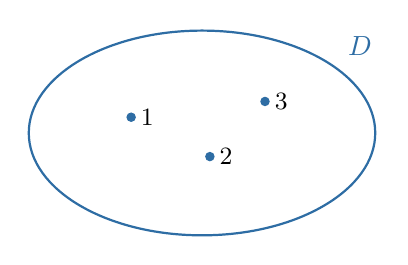
\begin{tikzpicture}
  % Ellipse for set D
  \draw[blu, thick] (0,0) ellipse (2.2cm and 1.3cm);
  % Label
  \node[blu, font=\bfseries] at (2.0, 1.1) {$D$};
  % Elements
  \filldraw[blu] (-0.9, 0.2) circle (1.5pt);
  \node at (-0.9, 0.2) [right, font=\small] {1};
  \filldraw[blu] (0.1, -0.3) circle (1.5pt);
  \node at (0.1, -0.3) [right, font=\small] {2};
  \filldraw[blu] (0.8, 0.4) circle (1.5pt);
  \node at (0.8, 0.4) [right, font=\small] {3};
\end{tikzpicture}
\end{center}
\end{esempio}

% ==============================================================
\section{Sottoinsiemi e inclusione}
% ==============================================================

\begin{definizione}
Dati due insiemi $A$ e $B$, si dice che $B$ è un \textbf{sottoinsieme} di $A$ — oppure che $B$ è \textbf{incluso} in $A$ — se \emph{ogni} elemento di $B$ appartiene anche ad $A$.

La notazione corretta è:
\[
  B \subseteq A
\]
che si legge «$B$ è incluso in $A$» oppure «$B$ è contenuto in $A$».

Se almeno un elemento di $B$ non appartiene ad $A$, si scrive $B \not\subseteq A$.
\end{definizione}

\begin{esempio}
Siano $A = \{1;\, 2;\, 3;\, 4;\, 5\}$ e $B = \{2;\, 4\}$.

Poiché $2 \in A$ e $4 \in A$, tutti gli elementi di $B$ appartengono ad $A$, quindi $B \subseteq A$.

\begin{center}
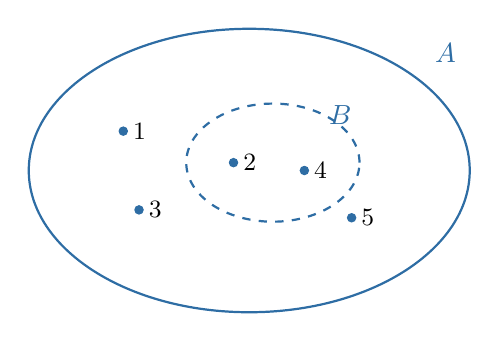
\begin{tikzpicture}
  % Outer ellipse A
  \draw[blu, thick] (0,0) ellipse (2.8cm and 1.8cm);
  \node[blu, font=\bfseries] at (2.5, 1.5) {$A$};
  % Elements of A outside B
  \filldraw[blu] (-1.6, 0.5) circle (1.5pt);
  \node at (-1.6, 0.5) [right, font=\small] {1};
  \filldraw[blu] (-1.4, -0.5) circle (1.5pt);
  \node at (-1.4,-0.5) [right, font=\small] {3};
  \filldraw[blu] (1.3, -0.6) circle (1.5pt);
  \node at (1.3,-0.6) [right, font=\small] {5};
  % Inner ellipse B
  \draw[blu, thick, dashed] (0.3, 0.1) ellipse (1.1cm and 0.75cm);
  \node[blu, font=\bfseries] at (1.15, 0.7) {$B$};
  % Elements of B
  \filldraw[blu] (-0.2, 0.1) circle (1.5pt);
  \node at (-0.2, 0.1) [right, font=\small] {2};
  \filldraw[blu] (0.7, 0.0) circle (1.5pt);
  \node at (0.7, 0.0) [right, font=\small] {4};
\end{tikzpicture}
\end{center}
\end{esempio}

\begin{attenzione}
\textbf{Attenzione!} L'insieme vuoto $\emptyset$ è sottoinsieme di \emph{qualsiasi} insieme. Ogni insieme è inoltre sottoinsieme di sé stesso: $A \subseteq A$.
\end{attenzione}

\begin{regola}
I simboli di inclusione e appartenenza hanno significati distinti e non possono essere confusi:
\begin{itemize}[leftmargin=1.5em]
  \item $\in$ collega un \emph{elemento} a un insieme: \quad $2 \in A$
  \item $\subseteq$ collega un \emph{insieme} a un altro insieme: \quad $B \subseteq A$
\end{itemize}
\end{regola}

% ==============================================================
\section{Operazioni con gli insiemi}
% ==============================================================

\subsection{Intersezione}

\begin{definizione}
L'\textbf{intersezione} di due insiemi $A$ e $B$ è il nuovo insieme che contiene \emph{tutti e soli} gli elementi che appartengono \textbf{sia} ad $A$ \textbf{sia} a $B$ (cioè gli elementi comuni).

La notazione corretta è:
\[
  A \cap B
\]
che si legge «$A$ \textbf{intersecato} $B$» oppure «$A$ inter $B$».
\end{definizione}

\begin{esempio}
Siano $A = \{1;\, 2;\, 3;\, 4;\, 5\}$ e $B = \{2;\, 4;\, 6;\, 8\}$.

Gli elementi comuni sono 2 e 4, quindi:
\[
  A \cap B = \{2;\, 4\}
\]

\begin{center}
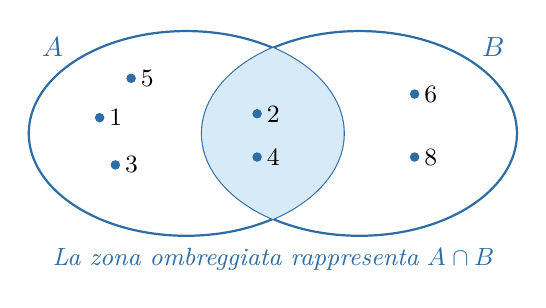
\begin{tikzpicture}
  % Ellipse A
  \draw[blu, thick] (-1.1, 0) ellipse (2.0cm and 1.3cm);
  \node[blu, font=\bfseries] at (-2.8, 1.1) {$A$};
  % Ellipse B
  \draw[blu, thick] (1.1, 0) ellipse (2.0cm and 1.3cm);
  \node[blu, font=\bfseries] at (2.8, 1.1) {$B$};
  % Shade intersection (approximate)
  \begin{scope}
    \clip (-1.1,0) ellipse (2.0cm and 1.3cm);
    \fill[azzurro] (1.1,0) ellipse (2.0cm and 1.3cm);
  \end{scope}
  % Elements only in A
  \filldraw[blu] (-2.2, 0.2) circle (1.5pt);
  \node at (-2.2, 0.2) [right, font=\small] {1};
  \filldraw[blu] (-2.0,-0.4) circle (1.5pt);
  \node at (-2.0,-0.4) [right, font=\small] {3};
  \filldraw[blu] (-1.8, 0.7) circle (1.5pt);
  \node at (-1.8, 0.7) [right, font=\small] {5};
  % Elements in intersection
  \filldraw[blu] (-0.2, 0.25) circle (1.5pt);
  \node at (-0.2, 0.25) [right, font=\small] {2};
  \filldraw[blu] (-0.2,-0.3) circle (1.5pt);
  \node at (-0.2,-0.3) [right, font=\small] {4};
  % Elements only in B
  \filldraw[blu] (1.8, 0.5) circle (1.5pt);
  \node at (1.8, 0.5) [right, font=\small] {6};
  \filldraw[blu] (1.8,-0.3) circle (1.5pt);
  \node at (1.8,-0.3) [right, font=\small] {8};
  % Label intersection
  \node[font=\small\itshape, blu] at (0, -1.6) {La zona ombreggiata rappresenta $A \cap B$};
\end{tikzpicture}
\end{center}
\end{esempio}

\begin{attenzione}
\textbf{Attenzione!} Se due insiemi non hanno elementi in comune, la loro intersezione è l'insieme vuoto: $A \cap B = \emptyset$. In questo caso si dice che $A$ e $B$ sono \textbf{disgiunti}.
\end{attenzione}

\subsection{Unione}

\begin{definizione}
L'\textbf{unione} di due insiemi $A$ e $B$ è il nuovo insieme che contiene \emph{tutti} gli elementi che appartengono ad $A$ \textbf{oppure} a $B$ \textbf{oppure} a entrambi.

La notazione corretta è:
\[
  A \cup B
\]
che si legge «$A$ \textbf{unito} $B$» oppure «$A$ union $B$».
\end{definizione}

\begin{esempio}
Siano $A = \{1;\, 2;\, 3\}$ e $B = \{2;\, 4;\, 5\}$.

Raccogliendo tutti gli elementi (senza ripetere quelli comuni):
\[
  A \cup B = \{1;\, 2;\, 3;\, 4;\, 5\}
\]

\begin{center}
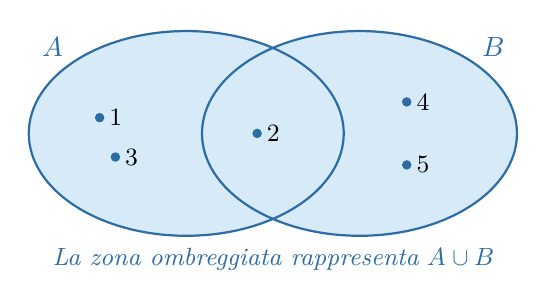
\begin{tikzpicture}
  % Shade entire union first
  \fill[azzurro] (-1.1, 0) ellipse (2.0cm and 1.3cm);
  \fill[azzurro] (1.1, 0) ellipse (2.0cm and 1.3cm);
  % Ellipse A
  \draw[blu, thick] (-1.1, 0) ellipse (2.0cm and 1.3cm);
  \node[blu, font=\bfseries] at (-2.8, 1.1) {$A$};
  % Ellipse B
  \draw[blu, thick] (1.1, 0) ellipse (2.0cm and 1.3cm);
  \node[blu, font=\bfseries] at (2.8, 1.1) {$B$};
  % Elements only in A
  \filldraw[blu] (-2.2, 0.2) circle (1.5pt);
  \node at (-2.2, 0.2) [right, font=\small] {1};
  \filldraw[blu] (-2.0,-0.3) circle (1.5pt);
  \node at (-2.0,-0.3) [right, font=\small] {3};
  % Elements in intersection
  \filldraw[blu] (-0.2, 0.0) circle (1.5pt);
  \node at (-0.2, 0.0) [right, font=\small] {2};
  % Elements only in B
  \filldraw[blu] (1.7, 0.4) circle (1.5pt);
  \node at (1.7, 0.4) [right, font=\small] {4};
  \filldraw[blu] (1.7,-0.4) circle (1.5pt);
  \node at (1.7,-0.4) [right, font=\small] {5};
  % Label
  \node[font=\small\itshape, blu] at (0, -1.6) {La zona ombreggiata rappresenta $A \cup B$};
\end{tikzpicture}
\end{center}
\end{esempio}

\begin{attenzione}
\textbf{Attenzione!} Nella rappresentazione per elencazione di $A \cup B$, ogni elemento va scritto \emph{una volta sola}, anche se appartiene a entrambi gli insiemi. Nell'esempio precedente, 2 appartiene sia ad $A$ che a $B$, ma compare una sola volta nell'unione.
\end{attenzione}

% ==============================================================
\section*{Riepilogo del capitolo}
% ==============================================================

\begin{sapevi}
\textbf{Lo sapevi?} Il matematico e filosofo Georg Cantor (1845–1918) è considerato il fondatore della teoria degli insiemi. Egli fu il primo a trattare matematicamente il concetto di infinito, dimostrando che esistono «infiniti più grandi di altri». Le sue idee, inizialmente contestate, sono oggi alla base di tutta la matematica moderna.
\end{sapevi}

\bigskip

\begin{tcolorbox}[
  enhanced,
  breakable,
  colback  = azzurro,
  colframe = blu,
  fonttitle = \bfseries,
  title    = Riepilogo,
  left=6pt, right=6pt, top=4pt, bottom=4pt, arc=4pt
]
\begin{itemize}[leftmargin=1.5em]
  \item Un \textbf{insieme} è un raggruppamento ben definito di elementi con una caratteristica comune; si indica con una lettera maiuscola.
  \item Un insieme può essere \textbf{finito}, \textbf{infinito} o \textbf{vuoto} ($\emptyset$ oppure $\{\}$).
  \item $x \in A$ significa che $x$ appartiene ad $A$; $x \notin A$ significa che non vi appartiene.
  \item Un insieme si può rappresentare \textbf{per elencazione} $\{a;\,b;\,c\}$, \textbf{per caratteristica} o tramite un \textbf{diagramma di Eulero-Venn}.
  \item $B \subseteq A$ indica che $B$ è un \textbf{sottoinsieme} di $A$: tutti gli elementi di $B$ appartengono ad $A$.
  \item L'\textbf{intersezione} $A \cap B$ contiene gli elementi comuni ad $A$ e $B$.
  \item L'\textbf{unione} $A \cup B$ contiene tutti gli elementi di $A$ e di $B$ (senza ripetizioni).
\end{itemize}
\end{tcolorbox}

% ============================================================
%  cap04_multipli_divisori.tex — Matemagica
%  Capitolo 4: Multipli, divisori, MCD e mcm
% ============================================================

\chapter{Multipli, divisori, MCD e mcm}

% --- Obiettivi di apprendimento ---
\section*{Obiettivi di apprendimento}
\begin{itemize}[leftmargin=1.5em]
    \item Comprendere il concetto di multiplo e di divisore di un numero naturale.
    \item Rappresentare insiemi di multipli e di divisori con la notazione insiemistica.
    \item Riconoscere i numeri primi e distinguerli dai numeri composti.
    \item Scomporre un numero naturale in fattori primi.
    \item Applicare i criteri di divisibilità per 2, 3, 4, 5, 6, 9, 10 e 25.
    \item Calcolare il minimo comune multiplo (mcm) e il massimo comune divisore (MCD)
          di due o più numeri.
    \item Conoscere le principali proprietà di mcm e MCD e applicarle.
\end{itemize}

% ============================================================
\section{I multipli di un numero naturale}
% ============================================================

\begin{definizione}
    I \textbf{multipli} di un numero naturale $n$ sono tutti i numeri naturali che si
    ottengono moltiplicando $n$ per ciascun numero naturale:
    \[
        n \times 0,\quad n \times 1,\quad n \times 2,\quad n \times 3,\quad \ldots
    \]
    I multipli di $n$ formano un insieme, indicato con il simbolo $M_n$, la cui
    caratteristica è \emph{«essere multiplo di $n$»}.
\end{definizione}

\begin{esempio}
    Alcuni insiemi di multipli:
    \begin{align*}
        M_3    & = \{0;\; 3;\; 6;\; 9;\; 12;\; 15;\; 18;\; 21;\; \ldots\} \\
        M_5    & = \{0;\; 5;\; 10;\; 15;\; 20;\; 25;\; 30;\; \ldots\}     \\
        M_{13} & = \{0;\; 13;\; 26;\; 39;\; \ldots\}
    \end{align*}
\end{esempio}

\begin{attenzione}
    \textbf{Attenzione.} Lo zero è multiplo di qualsiasi numero naturale, perché
    $n \times 0 = 0$ per ogni $n$. Tuttavia, quando si cerca il minimo comune multiplo
    si considera il più piccolo multiplo \emph{diverso da zero}.
\end{attenzione}

\begin{esempio}
    Rappresentare per elencazione i seguenti insiemi, usando la notazione insiemistica:

    \medskip
    \textbf{A} $= \{x \in \mathbb{N} \mid x \in M_3 \text{ e } x > 24\}$

    Si cercano i multipli di 3 maggiori di 24:
    $27 = 3 \times 9$, $30 = 3 \times 10$, $33 = 3 \times 11$, \ldots

    \[
        A = \{27;\; 30;\; 33;\; 36;\; \ldots\}
    \]

    \medskip
    \textbf{B} $= \{x \in \mathbb{N} \mid x \in M_5 \text{ e } 10 < x \leq 30\}$

    Si cercano i multipli di 5 compresi tra 10 (escluso) e 30 (incluso):

    \[
        B = \{15;\; 20;\; 25;\; 30\}
    \]

    \medskip
    \textbf{C} $= \{x \in \mathbb{N} \mid x \in M_{13} \text{ e } x < 13\}$

    Il più piccolo multiplo di 13 diverso da zero è 13 stesso. Non esistono multipli
    di 13 (positivi) inferiori a 13, quindi:

    \[
        C = \emptyset
    \]
\end{esempio}

% ============================================================
\section{Il minimo comune multiplo (mcm)}
% ============================================================

\begin{esempio}
    \textbf{Problema introduttivo — I pianeti in fila.}

    Giove e Mercurio sono due pianeti del sistema solare. Come la Terra, si muovono
    ruotando attorno al Sole: Giove compie un'orbita completa in 12 anni, Mercurio
    in 88 giorni. Adattiamo il problema ai nostri strumenti: supponiamo che Giove
    impieghi \textbf{4 anni} e Mercurio \textbf{6 anni} per compiere un'orbita.
    Se quest'anno si trovassero allineati rispetto al Sole, dopo quanti anni si
    ripeterebbe il fenomeno?

    \medskip
    I momenti di allineamento sono i multipli \emph{comuni} alle due durate:
    \begin{align*}
        M_4 & = \{0;\; 4;\; 8;\; \mathbf{12};\; 16;\; \ldots\} \\
        M_6 & = \{0;\; 6;\; \mathbf{12};\; 18;\; \ldots\}
    \end{align*}
    Il primo multiplo comune diverso da zero è \textbf{12}: i due pianeti si
    riallineano dopo 12 anni.
\end{esempio}

\begin{definizione}
    Il più piccolo multiplo \emph{diverso da zero} comune a due o più numeri si
    chiama \textbf{minimo comune multiplo} e si indica con \textbf{mcm}.
\end{definizione}

\begin{esempio}
    Trovare il mcm di 3 e 7 per enumerazione:
    \begin{align*}
        M_7 & = \{0;\; 7;\; 14;\; \mathbf{21};\; 28;\; \ldots\}                 \\
        M_3 & = \{0;\; 3;\; 6;\; 9;\; 12;\; 15;\; 18;\; \mathbf{21};\; \ldots\}
    \end{align*}
    Fra tutti i multipli comuni a 7 e 3, il più piccolo diverso da zero è 21,
    quindi $\text{mcm}(3;\, 7) = 21$.
\end{esempio}

% ============================================================
\section{I divisori di un numero naturale}
% ============================================================

\begin{definizione}
    I \textbf{divisori} di un numero naturale $n$ sono tutti i numeri naturali che
    dividono $n$ esattamente, cioè con resto zero. I divisori di $n$ formano un
    insieme, indicato con il simbolo $D_n$, la cui caratteristica è
    \emph{«essere divisore di $n$»}.
\end{definizione}

\begin{esempio}
    Alcuni insiemi di divisori:
    \begin{align*}
        D_6    & = \{1;\; 2;\; 3;\; 6\}                        \\
        D_{11} & = \{1;\; 11\}                                 \\
        D_{40} & = \{1;\; 2;\; 4;\; 5;\; 8;\; 10;\; 20;\; 40\}
    \end{align*}
\end{esempio}

\begin{esempio}
    Rappresentare per elencazione i seguenti insiemi:

    \medskip
    \textbf{A} $= \{x \in \mathbb{N} \mid x \in D_{15}\}$

    I divisori di 15 sono: $1 \times 15 = 15$, $3 \times 5 = 15$.
    \[
        A = \{1;\; 3;\; 5;\; 15\}
    \]

    \medskip
    \textbf{B} $= \{x \in \mathbb{N} \mid x \in D_{31}\}$

    Il numero 31 è divisibile solo per 1 e per se stesso (come vedremo, è un numero primo).
    \[
        B = \{1;\; 31\}
    \]

    \medskip
    \textbf{C} $= \{x \in \mathbb{N} \mid x \in D_{46} \text{ e } x < 23\}$

    I divisori di 46 sono: $\{1;\; 2;\; 23;\; 46\}$. Fra questi, quelli minori di 23 sono:
    \[
        C = \{1;\; 2\}
    \]
\end{esempio}

\begin{attenzione}
    \textbf{I divisori sono in numero finito.} Ogni numero naturale $n > 0$ ha un
    numero limitato di divisori: essi sono compresi tra 1 e $n$.
    I multipli di un numero, invece, sono infiniti.
\end{attenzione}

% ============================================================
\section{Numeri primi e numeri composti}
% ============================================================

Osservando gli insiemi dei divisori, emerge una distinzione importante.

\begin{definizione}
    Un numero naturale maggiore di 1 si dice \textbf{numero primo} se ha esattamente
    due divisori: 1 e se stesso.

    Un numero naturale maggiore di 1 che ha più di due divisori si dice
    \textbf{numero composto}.

    Il numero 1 non è né primo né composto: è un caso a parte, con un solo divisore.
\end{definizione}

\begin{esempio}
    \begin{itemize}[leftmargin=1.5em]
        \item $D_7 = \{1;\; 7\}$ \quad — 7 è \textbf{primo} \quad\textit{(corretto)}
        \item $D_{13} = \{1;\; 13\}$ \quad — 13 è \textbf{primo} \quad\textit{(corretto)}
        \item $D_{12} = \{1;\; 2;\; 3;\; 4;\; 6;\; 12\}$ \quad — 12 è \textbf{composto} \quad\textit{(corretto)}
        \item $D_1 = \{1\}$ \quad — 1 non è né primo né composto
    \end{itemize}
\end{esempio}

I primi numeri primi sono:
\[
    2,\; 3,\; 5,\; 7,\; 11,\; 13,\; 17,\; 19,\; 23,\; 29,\; 31,\; 37,\; 41,\; 43,\; 47,\; \ldots
\]

\begin{attenzione}
    \textbf{Il 2 è l'unico numero primo pari.} Ogni altro numero pari è divisibile per 2
    (oltre che per 1 e per se stesso), quindi ha più di due divisori ed è composto.
\end{attenzione}

\begin{sapevi}
    \textbf{Il crivello di Eratostene.}
    Eratostene di Cirene (276–194 a.C.), matematico e geografo greco, ideò un metodo
    elegante per trovare tutti i numeri primi fino a un certo valore. Si scrivono
    tutti i numeri da 2 in poi; si tiene il 2 (primo) e si eliminano tutti i suoi
    multipli; si tiene il successivo non eliminato (3) e si eliminano tutti i suoi
    multipli; e così via. I numeri che rimangono sono esattamente i numeri primi.
    Questo metodo è ancora oggi usato in informatica per generare liste di numeri primi.
\end{sapevi}

% ============================================================
\section{La scomposizione in fattori primi}
% ============================================================

\begin{definizione}
    Ogni numero naturale maggiore di 1 può essere scritto come prodotto di numeri
    primi, detti \textbf{fattori primi}. Questa scrittura si chiama
    \textbf{scomposizione in fattori primi} (o \textbf{fattorizzazione}).
    La scomposizione in fattori primi di un numero è \emph{unica}
    (a meno dell'ordine dei fattori).
\end{definizione}

Il metodo pratico consiste nel dividere il numero per il più piccolo fattore
primo che lo divide esattamente, poi ripetere con il quoziente ottenuto, fino
ad arrivare a 1.

\begin{esempio}
    Scomporre 60 in fattori primi.

    Si procede con divisioni successive:

    \[
        \begin{array}{r|l}
            60 & 2 \\
            30 & 2 \\
            15 & 3 \\
            5  & 5 \\
            1  &
        \end{array}
    \]

    Quindi: $60 = 2 \times 2 \times 3 \times 5 = 2^2 \times 3 \times 5$
    \quad\textit{(corretto)}
\end{esempio}

\begin{esempio}
    Scomporre 84 in fattori primi.

    \[
        \begin{array}{r|l}
            84 & 2 \\
            42 & 2 \\
            21 & 3 \\
            7  & 7 \\
            1  &
        \end{array}
    \]

    Quindi: $84 = 2^2 \times 3 \times 7$
    \quad\textit{(corretto)}
\end{esempio}

\begin{attenzione}
    \textbf{Come scegliere il divisore primo.} Si comincia sempre dal numero primo
    più piccolo (2), e si passa al successivo solo quando il quoziente non è più
    divisibile per il primo corrente. L'ordine è: 2, 3, 5, 7, 11, 13, \ldots

    Se non si è sicuri che un numero sia primo, si prova a dividerlo per tutti i
    numeri primi fino alla sua radice quadrata: se nessuno lo divide, allora è primo.
\end{attenzione}

% ============================================================
\section{I criteri di divisibilità}
% ============================================================

Trovare i divisori di un numero grande può essere complicato. I \textbf{criteri
    di divisibilità} permettono di stabilire rapidamente se un numero è divisibile
per un altro, senza eseguire la divisione.

\begin{regola}
    \begin{itemize}[leftmargin=1.5em]
        \item Un numero è divisibile per \textbf{2} se è pari (cioè termina con
              0, 2, 4, 6 o 8).
        \item Un numero è divisibile per \textbf{3} se la somma delle sue cifre
              è divisibile per 3.
        \item Un numero è divisibile per \textbf{4} se il numero formato dalle
              sue ultime due cifre è divisibile per 4.
        \item Un numero è divisibile per \textbf{5} se termina con 0 o con 5.
        \item Un numero è divisibile per \textbf{6} se è divisibile per 2 e per 3
              contemporaneamente.
        \item Un numero è divisibile per \textbf{9} se la somma delle sue cifre
              è divisibile per 9.
        \item Un numero è divisibile per \textbf{10} se termina con 0.
        \item Un numero è divisibile per \textbf{25} se termina con 00, 25, 50 o 75.
    \end{itemize}
\end{regola}

\begin{esempio}
    Verificare la divisibilità di 5\,748 applicando i criteri.

    \begin{itemize}[leftmargin=1.5em]
        \item \textbf{Per 2:} termina con 8 (cifra pari) \quad$\Rightarrow$\quad
              divisibile \quad\textit{(corretto)}
        \item \textbf{Per 3:} $5 + 7 + 4 + 8 = 24$, e $24 \div 3 = 8$ \quad$\Rightarrow$\quad
              divisibile \quad\textit{(corretto)}
        \item \textbf{Per 4:} le ultime due cifre sono 48, e $48 \div 4 = 12$ \quad$\Rightarrow$\quad
              divisibile \quad\textit{(corretto)}
        \item \textbf{Per 5:} termina con 8 \quad$\Rightarrow$\quad
              non divisibile
        \item \textbf{Per 6:} divisibile per 2 e per 3 \quad$\Rightarrow$\quad
              divisibile \quad\textit{(corretto)}
        \item \textbf{Per 9:} $5 + 7 + 4 + 8 = 24$, e $24 \div 9$ non è esatto \quad$\Rightarrow$\quad
              non divisibile
        \item \textbf{Per 10:} non termina con 0 \quad$\Rightarrow$\quad
              non divisibile
    \end{itemize}
\end{esempio}

\begin{sapevi}
    \textbf{Perché funziona il criterio del 9?}
    Ogni numero può essere scritto come somma di potenze di 10:
    per esempio $345 = 3 \times 100 + 4 \times 10 + 5$. Poiché
    $10 = 9 + 1$, $100 = 99 + 1$, ecc., si può dimostrare che un numero e la
    somma delle sue cifre danno lo stesso resto quando vengono divisi per 9.
    Lo stesso ragionamento vale per il criterio del 3.
\end{sapevi}

% ============================================================
\section{Il massimo comune divisore (MCD)}
% ============================================================

\begin{definizione}
    Il più grande divisore comune a due o più numeri si chiama
    \textbf{massimo comune divisore} e si indica con \textbf{MCD}.
\end{definizione}

\begin{esempio}
    Trovare il MCD di 16 e 64 per enumerazione:
    \begin{align*}
        D_{16} & = \{1;\; 2;\; 4;\; 8;\; \mathbf{16}\}             \\
        D_{64} & = \{1;\; 2;\; 4;\; 8;\; \mathbf{16};\; 32;\; 64\}
    \end{align*}
    Fra tutti i divisori comuni a 16 e 64, il più grande è 16,
    quindi $\text{MCD}(16;\, 64) = 16$.
\end{esempio}

% ============================================================
\section{Calcolo di mcm e MCD con la scomposizione in fattori primi}
% ============================================================

Il metodo per enumerazione funziona bene con numeri piccoli, ma diventa
impraticabile con numeri grandi. Il metodo più efficiente si basa sulla
scomposizione in fattori primi.

\begin{regola}
    \textbf{Calcolo del MCD.}
    \begin{enumerate}[leftmargin=1.5em]
        \item Scomporre ciascun numero in fattori primi.
        \item Individuare i fattori primi \emph{comuni} a tutte le scomposizioni.
        \item Il MCD è il prodotto di quei fattori comuni, ciascuno preso con
              l'\emph{esponente minore}.
    \end{enumerate}

    \textbf{Calcolo del mcm.}
    \begin{enumerate}[leftmargin=1.5em]
        \item Scomporre ciascun numero in fattori primi.
        \item Raccogliere \emph{tutti} i fattori primi che compaiono in almeno
              una scomposizione.
        \item Il mcm è il prodotto di tutti quei fattori, ciascuno preso con
              l'\emph{esponente maggiore}.
    \end{enumerate}
\end{regola}

\begin{esempio}
    Calcolare MCD e mcm di 180 e 252.

    \medskip
    \textbf{Passo 1 — scomposizione in fattori primi:}

    \[
        \begin{array}{r|l}
            180 & 2 \\
            90  & 2 \\
            45  & 3 \\
            15  & 3 \\
            5   & 5 \\
            1   &
        \end{array}
        \qquad\Rightarrow\qquad
        180 = 2^2 \times 3^2 \times 5
    \]

    \[
        \begin{array}{r|l}
            252 & 2 \\
            126 & 2 \\
            63  & 3 \\
            21  & 3 \\
            7   & 7 \\
            1   &
        \end{array}
        \qquad\Rightarrow\qquad
        252 = 2^2 \times 3^2 \times 7
    \]

    \medskip
    \textbf{Passo 2 — MCD} (fattori comuni con esponente minore):

    I fattori comuni sono 2 e 3. L'esponente minore di 2 è 2; l'esponente minore di 3 è 2.

    \[
        \text{MCD}(180;\, 252) = 2^2 \times 3^2 = 4 \times 9 = 36
    \]

    \textbf{Passo 3 — mcm} (tutti i fattori con esponente maggiore):

    I fattori che compaiono sono 2, 3, 5 e 7.

    \[
        \text{mcm}(180;\, 252) = 2^2 \times 3^2 \times 5 \times 7 = 4 \times 9 \times 5 \times 7 = 1260
    \]
\end{esempio}

\begin{attenzione}
    \textbf{Errore comune.} Nel calcolo del MCD si prendono \emph{solo} i fattori
    \emph{comuni} con l'esponente \emph{minore}. Nel calcolo del mcm si prendono
    \emph{tutti} i fattori (anche quelli non comuni) con l'esponente \emph{maggiore}.
    Confondere i due criteri è l'errore più frequente.
\end{attenzione}

% ============================================================
\section{Proprietà di mcm e MCD}
% ============================================================

\begin{regola}
    Le seguenti proprietà permettono di semplificare molti calcoli:

    \begin{enumerate}[leftmargin=1.5em]
        \item \textbf{Numeri coprimi.} Se MCD$(a;\, b) = 1$, i due numeri si dicono
              \textbf{coprimi} (o primi tra loro). In questo caso:
              \[
                  \text{mcm}(a;\, b) = a \times b
              \]
              \textit{Esempio:} MCD$(4;\, 9) = 1$, quindi mcm$(4;\, 9) = 36$.

        \item \textbf{Se $a$ divide $b$.} Se $a$ è divisore di $b$, allora:
              \[
                  \text{MCD}(a;\, b) = a \qquad \text{e} \qquad \text{mcm}(a;\, b) = b
              \]
              \textit{Esempio:} MCD$(4;\, 12) = 4$ e mcm$(4;\, 12) = 12$.

        \item \textbf{Relazione tra MCD e mcm.} Per due numeri qualsiasi $a$ e $b$:
              \[
                  \text{MCD}(a;\, b) \times \text{mcm}(a;\, b) = a \times b
              \]
              \textit{Esempio:} $a = 12$, $b = 18$:
              $\text{MCD} = 6$, $\text{mcm} = 36$,
              e infatti $6 \times 36 = 216 = 12 \times 18$. \quad\textit{(corretto)}

        \item \textbf{Il MCD è sempre minore o uguale al più piccolo dei numeri.}
              Il mcm è sempre maggiore o uguale al più grande dei numeri.
    \end{enumerate}
\end{regola}

\begin{sapevi}
    \textbf{mcm e MCD nella vita quotidiana.}
    Il minimo comune multiplo non serve solo per i pianeti. Si usa ogni volta che
    bisogna sincronizzare eventi che si ripetono con periodicità diversa: i turni
    di lavoro, le finestre di manutenzione di macchine industriali, oppure —
    in musica — per trovare il momento in cui due ritmi diversi tornano a coincidere.
    Il MCD, invece, è alla base del calcolo delle frazioni equivalenti e della
    semplificazione delle frazioni, concetti che affronteremo nel prossimo capitolo.
\end{sapevi}

% ============================================================
\section*{Riepilogo}
% ============================================================

\begin{regola}
    \textbf{Riepilogo del capitolo.}

    \begin{itemize}[leftmargin=1.5em]
        \item I \textbf{multipli} di $n$ sono i prodotti $n \times 0,\; n \times 1,\;
                  n \times 2,\; \ldots$ e formano l'insieme $M_n$ (infinito).
        \item I \textbf{divisori} di $n$ sono i numeri naturali che dividono $n$
              esattamente e formano l'insieme $D_n$ (finito).
        \item Un numero con esattamente due divisori è \textbf{primo}; con più di
              due è \textbf{composto}; il numero 1 non è né primo né composto.
        \item Ogni numero composto si scompone in modo unico come prodotto di
              \textbf{fattori primi}.
        \item I \textbf{criteri di divisibilità} permettono di riconoscere
              rapidamente i divisori di 2, 3, 4, 5, 6, 9, 10 e 25.
        \item Il \textbf{MCD} si calcola moltiplicando i fattori primi comuni con
              l'esponente \emph{minore}.
        \item Il \textbf{mcm} si calcola moltiplicando tutti i fattori primi con
              l'esponente \emph{maggiore}.
        \item Per due numeri $a$ e $b$: $\text{MCD}(a;\,b) \times \text{mcm}(a;\,b)
                  = a \times b$.
    \end{itemize}
\end{regola}
% ============================================================
%  cap05_espressioni.tex — Matemagica
%  Capitolo 5: Espressioni aritmetiche
% ============================================================

\chapter{Espressioni aritmetiche}

% --- Obiettivi di apprendimento ---
\section*{Obiettivi di apprendimento}
\begin{itemize}[leftmargin=1.5em]
    \item Comprendere il concetto di espressione aritmetica.
    \item Applicare correttamente le regole di precedenza tra le operazioni.
    \item Risolvere espressioni con parentesi tonde, quadre e graffe.
    \item Distinguere i due ruoli delle parentesi graffe: notazione insiemistica
          e raggruppamento nelle espressioni.
    \item Confrontare la notazione con sole parentesi tonde annidate e quella
          con i tre ordini di parentesi.
\end{itemize}

% ============================================================
\section{Che cos'è un'espressione aritmetica}
% ============================================================

\begin{definizione}
    Un'\textbf{espressione aritmetica} è una scrittura matematica che collega
    due o più numeri tramite segni di operazione. È una catena di operazioni il
    cui risultato finale è un unico numero, detto \textbf{valore dell'espressione}.
\end{definizione}

\begin{esempio}
    Le seguenti sono espressioni aritmetiche:
    \[
        12 + 5 \times 3 \qquad\qquad
        (8 - 2) \times 4 + 6 : 2 \qquad\qquad
        \{3 \times [10 - (2 + 1)]\} + 5
    \]
\end{esempio}

\begin{attenzione}
    \textbf{Un'espressione non è un'equazione.} Un'espressione aritmetica non
    contiene il segno di uguale: va \emph{calcolata}, non \emph{risolta}.
    Il segno $=$ appare solo nei passaggi intermedi che mostriamo durante il calcolo.
\end{attenzione}

% ============================================================
\section{Le regole di precedenza}
% ============================================================

Per ottenere un risultato univoco, ogni persona che calcola la stessa
espressione deve seguire le stesse regole. Queste si chiamano
\textbf{regole di precedenza}.

\begin{regola}
    \textbf{Ordine di esecuzione delle operazioni.}
    \begin{enumerate}[leftmargin=1.5em]
        \item Si risolvono prima le operazioni racchiuse fra \textbf{parentesi},
              cominciando da quelle più interne.
        \item Fra le operazioni senza parentesi, \textbf{moltiplicazione} e
              \textbf{divisione} hanno la precedenza su addizione e sottrazione.
        \item Fra operazioni dello stesso livello (solo addizioni e sottrazioni,
              oppure solo moltiplicazioni e divisioni) si procede
              \textbf{da sinistra verso destra}.
    \end{enumerate}
\end{regola}

\begin{esempio}
    Calcolare $12 + 5 \times 3 - 8 : 4$.

    Non ci sono parentesi, quindi si eseguono prima le moltiplicazioni e le divisioni,
    da sinistra verso destra, poi le addizioni e le sottrazioni:
    \begin{align*}
        12 + 5 \times 3 - 8 : 4
         & = 12 + 15 - 2 \\
         & = 27 - 2      \\
         & = 25
    \end{align*}
\end{esempio}

\begin{attenzione}
    \textbf{Errore comune — procedere semplicemente da sinistra verso destra.}
    Senza rispettare le precedenze, $12 + 5 \times 3$ potrebbe essere calcolato
    come $(12 + 5) \times 3 = 51$, risultato scorretto.
    La risposta corretta è $12 + 15 = 27$, perché la moltiplicazione precede
    l'addizione. \quad\textit{(corretto)}
\end{attenzione}

% ============================================================
\section{Le parentesi nelle espressioni}
% ============================================================

Le parentesi servono a modificare l'ordine naturale delle operazioni:
tutto ciò che è racchiuso fra una coppia di parentesi va calcolato
\emph{prima} del resto.

\subsection{Parentesi tonde annidate}

Il modo più semplice di indicare più livelli di raggruppamento è usare
più coppie di parentesi \textbf{tonde}, una dentro l'altra.
Questa scrittura si dice \textbf{annidata} (dal latino \emph{nidus}, nido:
ogni coppia di parentesi «contiene» quella più interna come un nido).

\begin{regola}
    Con le sole parentesi tonde annidate, si procede sempre dalla
    \textbf{parentesi più interna} verso quella più esterna.
\end{regola}

\begin{esempio}
    Calcolare $((3 + 2) \times (4 - 1) + 6) \times 2$.

    Si individua la parentesi più esterna e si lavora dall'interno:
    \begin{align*}
        ((3 + 2) \times (4 - 1) + 6) \times 2
         & = (5 \times 3 + 6) \times 2 &  & \text{[parentesi più interne]}     \\
         & = (15 + 6) \times 2         &  & \text{[moltiplicazione]}           \\
         & = 21 \times 2               &  & \text{[addizione nella parentesi]} \\
         & = 42
    \end{align*}
\end{esempio}

\begin{attenzione}
    \textbf{La notazione con sole tonde annidate è corretta ma poco leggibile.}
    Espressioni come $((8-(3+1))\times(5-(2+1)))+4$ sono difficili da leggere:
    è faticoso contare quante parentesi si aprono e quante si chiudono,
    e un errore di conteggio porta a un risultato sbagliato.
    Per questo motivo, nella pratica matematica si usa una notazione più chiara,
    basata su tre tipi di parentesi distinte.
\end{attenzione}

\subsection{I tre ordini di parentesi: tonde, quadre e graffe}

Per rendere le espressioni più leggibili e meno soggette a errori di lettura,
la matematica utilizza tre simboli distinti, usati dall'interno verso l'esterno:

\begin{center}
    \begin{tabular}{cll}
        \toprule
        \textbf{Simbolo} & \textbf{Nome}             & \textbf{Livello}    \\
        \midrule
        $(\quad)$        & Parentesi \textbf{tonde}  & Primo (più interno) \\
        $[\quad]$        & Parentesi \textbf{quadre} & Secondo             \\
        $\{\quad\}$      & Parentesi \textbf{graffe} & Terzo (più esterno) \\
        \bottomrule
    \end{tabular}
\end{center}

\begin{regola}
    Con i tre ordini di parentesi, si procede sempre dall'interno verso
    l'esterno, rispettando la gerarchia:
    \[
        \text{tonde} \longrightarrow \text{quadre} \longrightarrow \text{graffe}
    \]
    All'interno di ciascuna coppia di parentesi valgono le normali regole
    di precedenza: prima moltiplicazioni e divisioni, poi addizioni e sottrazioni.
\end{regola}

\begin{esempio}
    Calcolare $\{3 \times [10 - (2 + 1)] + 5\} : 4$.

    \textbf{Passo 1} — parentesi tonde (più interne):
    \[
        \{3 \times [10 - 3] + 5\} : 4
    \]
    \textbf{Passo 2} — parentesi quadre:
    \[
        \{3 \times 7 + 5\} : 4
        = \{21 + 5\} : 4
        = \{26\} : 4
    \]
    \textbf{Passo 3} — parentesi graffe:
    \[
        26 : 4 = 6{,}5
    \]
\end{esempio}

\begin{esempio}
    Calcolare $\{5 \times [(12 - 4) : (3 - 1)] - 2\} + 3 \times 4$.

    \textbf{Passo 1} — parentesi tonde (ce ne sono due, allo stesso livello):
    \begin{align*}
        \{5 \times [8 : 2] - 2\} + 3 \times 4
    \end{align*}
    \textbf{Passo 2} — parentesi quadre:
    \begin{align*}
        \{5 \times 4 - 2\} + 3 \times 4
        = \{20 - 2\} + 3 \times 4
        = \{18\} + 3 \times 4
    \end{align*}
    \textbf{Passo 3} — fuori da tutte le parentesi, moltiplicazione prima:
    \begin{align*}
        18 + 12 = 30
    \end{align*}
\end{esempio}

% ============================================================
\section{Confronto tra i due approcci}
% ============================================================

Come abbiamo visto, le due notazioni sono \textbf{equivalenti dal punto di
    vista matematico}: producono lo stesso risultato. La differenza è nella
leggibilità.

\begin{center}
    \begin{tabular}{p{0.42\linewidth} p{0.42\linewidth}}
        \toprule
        \textbf{Solo parentesi tonde annidate}                                    & \textbf{Tre ordini di parentesi} \\
        \midrule
        $((8-(3+1))\times(5-(2+1)))+4$                                            &
        $\{[8-(3+1)]\times[5-(2+1)]\}+4$                                                                             \\[4pt]
        Tutte le parentesi hanno la stessa forma: più livelli ci sono,
        più è difficile distinguerli a colpo d'occhio.                            &
        Ogni livello ha un simbolo diverso: è immediato vedere quale operazione
        va risolta prima.                                                                                            \\[4pt]
        Richiede di contare attentamente l'apertura e la chiusura di ogni coppia. &
        La forma visiva guida la lettura e riduce gli errori.                                                        \\
        \bottomrule
    \end{tabular}
\end{center}

\begin{sapevi}
    \textbf{Un doppio ruolo per le parentesi graffe.}

    Nel capitolo sugli insiemi abbiamo usato le parentesi graffe per elencare
    gli elementi di un insieme: $A = \{1;\; 3;\; 5\}$.
    Nelle espressioni aritmetiche, le stesse graffe svolgono un ruolo diverso:
    indicano il livello più esterno di raggruppamento.

    I due usi si distinguono dal contesto:
    \begin{itemize}[leftmargin=1.5em]
        \item Se le graffe contengono un elenco di numeri separati da punto e
              virgola, si tratta di un \textbf{insieme}.
        \item Se le graffe contengono un'operazione, si tratta di un
              \textbf{raggruppamento} in un'espressione.
    \end{itemize}
    In matematica è frequente che uno stesso simbolo abbia significati diversi
    a seconda del contesto: riconoscere il contesto è parte del ragionamento
    matematico.
\end{sapevi}

% ============================================================
\section{Le parentesi e la proprietà distributiva}
% ============================================================

Le parentesi non servono solo a stabilire l'ordine delle operazioni:
hanno anche un legame profondo con la \textbf{proprietà distributiva}
della moltiplicazione rispetto all'addizione e alla sottrazione.

\begin{regola}
    \textbf{Proprietà distributiva.}
    \[
        a \times (b + c) = a \times b + a \times c
        \qquad\qquad
        a \times (b - c) = a \times b - a \times c
    \]
    Questo significa che una moltiplicazione che «abbraccia» una somma
    (o una differenza) può essere distribuita su ciascun termine.
\end{regola}

\begin{esempio}
    Verificare che $4 \times (5 + 3) = 4 \times 5 + 4 \times 3$.
    \begin{align*}
        4 \times (5 + 3)        & = 4 \times 8 = 32                       \\
        4 \times 5 + 4 \times 3 & = 20 + 12 = 32 \quad\textit{(corretto)}
    \end{align*}
\end{esempio}

\begin{attenzione}
    \textbf{La proprietà distributiva NON vale per la divisione a sinistra.}
    \[
        (8 + 4) : 2 = 12 : 2 = 6
        \qquad\text{ma}\qquad
        8 : 2 + 4 : 2 = 4 + 2 = 6 \quad \text{(in questo caso funziona)}
    \]
    \[
        12 : (4 + 2) = 12 : 6 = 2
        \qquad\text{ma}\qquad
        12 : 4 + 12 : 2 = 3 + 6 = 9 \quad \text{(risultato diverso!)}
    \]
    Quando il \emph{divisore} contiene una somma racchiusa fra parentesi,
    la distribuzione non è applicabile.
\end{attenzione}

% ============================================================
\section*{Approfondimento — La convenzione internazionale}
% ============================================================

\begin{sapevi}
    \textbf{La posizione dell'American Physical Society.}

    L'\emph{American Physical Society} (APS), una delle principali organizzazioni
    scientifiche mondiali, ha codificato nelle proprie linee guida editoriali la
    convenzione che da secoli i matematici adottano per le parentesi nelle
    espressioni complesse.

    La regola stabilisce che, quando la forma delle parentesi non ha un significato
    speciale (come accade nelle espressioni aritmetiche), si deve lavorare
    dall'interno verso l'esterno seguendo la sequenza:
    \[
        \{ \;[\; (\quad) \;]\; \}
    \]
    e che \textbf{l'annidamento di sole parentesi tonde va evitato},
    perché rende la struttura dell'espressione difficile da leggere e da verificare.

    Questa non è una preferenza stilistica: è una convenzione che riduce
    gli errori e garantisce che la stessa espressione venga letta nello stesso
    modo da chiunque, indipendentemente dalla lingua o dalla scuola di appartenenza.
    Il fatto che alcuni testi scolastici introducano solo le parentesi tonde
    annidate è quindi una semplificazione didattica temporanea, non una regola
    matematica definitiva.
\end{sapevi}

% ============================================================
\section*{Riepilogo}
% ============================================================

\begin{regola}
    \textbf{Riepilogo del capitolo.}
    \begin{itemize}[leftmargin=1.5em]
        \item Un'\textbf{espressione aritmetica} è una catena di operazioni il
              cui calcolo segue regole precise.
        \item \textbf{Regole di precedenza}: prima le parentesi (dall'interno
              verso l'esterno), poi moltiplicazione e divisione, infine addizione
              e sottrazione; a parità di livello, da sinistra verso destra.
        \item Le parentesi si usano in tre ordini: \textbf{tonde} $(\,)$,
              \textbf{quadre} $[\,]$, \textbf{graffe} $\{\,\}$.
        \item Le due notazioni (sole tonde annidate / tre ordini) sono
              matematicamente equivalenti, ma la notazione a tre ordini è
              più leggibile e corrisponde alla convenzione internazionale.
        \item Le parentesi \textbf{graffe} hanno un doppio ruolo: indicano
              un insieme (con elementi separati da punto e virgola) oppure
              il livello più esterno di raggruppamento in un'espressione.
        \item La \textbf{proprietà distributiva} lega parentesi e
              moltiplicazione: $a \times (b + c) = a \times b + a \times c$.
    \end{itemize}
\end{regola}

% ============================================================
%  cap_potenze.tex — Le potenze
%  Matemagica — Scuole medie Canton Ticino (DECS)
% ============================================================

\chapter{Le potenze}

% --- Obiettivi di apprendimento --------------------------------
\section*{Obiettivi di apprendimento}
\begin{itemize}[leftmargin=1.5em]
  \item Comprendere il significato di \textbf{potenza} come moltiplicazione ripetuta.
  \item Conoscere e applicare le \textbf{proprietà delle potenze}.
  \item Riconoscere la precedenza dell'elevamento a potenza nelle espressioni aritmetiche.
  \item Leggere e scrivere numeri grandi utilizzando le \textbf{potenze di 10}.
  \item Comprendere i principi di base della \textbf{notazione scientifica}.
\end{itemize}

% ============================================================
\section{Dalla moltiplicazione alla potenza}
% ============================================================

\subsection{La riproduzione batterica}

I batteri sono microrganismi unicellulari che si riproducono dividendosi a metà:
da ogni divisione derivano due batteri, ognuno dei quali si divide di nuovo, e così via.
Immagina di partire da un singolo batterio che si riproduce ogni ora.

\begin{center}
  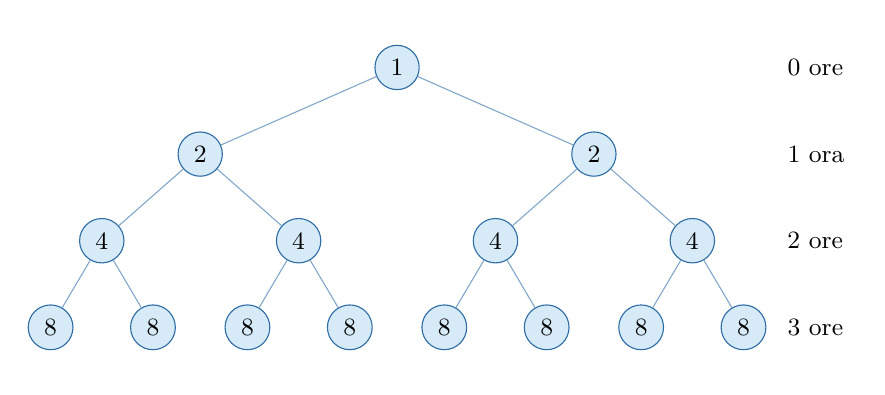
\begin{tikzpicture}[
      every node/.style={circle, draw=blu, fill=azzurro, inner sep=3pt, font=\small},
      level distance=1.1cm,
      level 1/.style={sibling distance=5cm},
      level 2/.style={sibling distance=2.5cm},
      level 3/.style={sibling distance=1.3cm},
      edge from parent/.style={draw=blu!60, thin}
    ]
    \node {1}
    child { node {2}
        child { node {4}
            child { node {8} }
            child { node {8} }
          }
        child { node {4}
            child { node {8} }
            child { node {8} }
          }
      }
    child { node {2}
        child { node {4}
            child { node {8} }
            child { node {8} }
          }
        child { node {4}
            child { node {8} }
            child { node {8} }
          }
      };
    % Etichette ore
    \node[draw=none, fill=none, right=0.3cm] at (4.5, 0)    {\small 0 ore};
    \node[draw=none, fill=none, right=0.3cm] at (4.5, -1.1) {\small 1 ora};
    \node[draw=none, fill=none, right=0.3cm] at (4.5, -2.2) {\small 2 ore};
    \node[draw=none, fill=none, right=0.3cm] at (4.5, -3.3) {\small 3 ore};
  \end{tikzpicture}
\end{center}

Quanti batteri ci sono dopo 5 ore? Bisogna moltiplicare 2 per sé stesso 5 volte:
\[
  2 \cdot 2 \cdot 2 \cdot 2 \cdot 2 = 32
\]

Che calcoli lunghi! Esiste però un modo per abbreviare una \textbf{moltiplicazione
  di fattori tutti uguali}: si chiama \textbf{elevazione a potenza}.

\begin{center}
  \begin{tabular}{@{} c c r @{}}
    \toprule
    \textbf{Ore trascorse} & \textbf{Moltiplicazione}                      & \textbf{Numero di batteri} \\
    \midrule
    0                      & $2^0$                                         & 1                          \\
    1                      & $2^1$                                         & 2                          \\
    2                      & $2 \times 2 = 2^2$                            & 4                          \\
    3                      & $2 \times 2 \times 2 = 2^3$                   & 8                          \\
    4                      & $2 \times 2 \times 2 \times 2 = 2^4$          & 16                         \\
    5                      & $2 \times 2 \times 2 \times 2 \times 2 = 2^5$ & 32                         \\
    12                     & $2^{12}$                                      & 4096                       \\
    \bottomrule
  \end{tabular}
\end{center}

\begin{sapevi}
  \textbf{Lo sapevi?}

  Lo yogurt che mangi a colazione esiste grazie ai batteri! Alcuni tipi di batteri
  «buoni», detti \textit{fermenti lattici}, trasformano il latte in yogurt attraverso
  un processo di fermentazione. Senza la riproduzione batterica — e senza le potenze
  per descriverla — non potremmo capire quanto rapidamente avviene questo processo.
\end{sapevi}

% ============================================================
\subsection{Perché servono le potenze? Tre storie matematiche}
% ============================================================

Le potenze non sono un'invenzione recente: i matematici le hanno usate (senza
saperlo) per migliaia di anni. Ecco tre esempi tratti dalla storia.

\subsubsection*{La scacchiera del bramino}

\begin{sapevi}
  \textbf{L'invenzione del gioco degli scacchi}

  Secondo un antico racconto, il re Iadava perse il suo unico figlio durante una guerra
  e cadde in una profonda disperazione. Un giorno, un umile bramino gli donò una tavola
  divisa in 64 caselle: era la scacchiera. Il re apprezzò talmente il gioco da chiedere
  al bramino come volesse essere ricompensato.

  Il bramino rispose: «Non voglio oro, terreni o palazzi. Mi darai un chicco di grano
  per la prima casella, due per la seconda, quattro per la terza, e così via,
  raddoppiando la quantità ad ogni casella fino all'ultima.»

  Il re rise: sembrava una richiesta da sciocco. Ma i matematici di corte calcolarono
  la verità. Il numero totale di chicchi richiesti è:
  \[
    1 + 2 + 2^2 + 2^3 + \cdots + 2^{63} = 2^{64} - 1 = 18\,446\,744\,073\,709\,551\,615
  \]
  Circa $1{,}8 \times 10^{19}$ chicchi — più di tutta la produzione mondiale di grano
  per migliaia di anni. Il bramino non era affatto uno sciocco!

  \textit{Adattato da: Malba Tahan, \textup{L'uomo che sapeva contare}, Salani.}
\end{sapevi}

\subsubsection*{I sette gatti di Ahmes}

Il seguente problema è contenuto nel \textbf{Papiro di Ahmes}, un documento egizio
del 1700 a.C. conservato al British Museum di Londra — uno dei testi matematici
più antichi del mondo.

\begin{esempio}
  \textit{In ogni casa ci sono sette gatti.
    Ogni gatto acchiappa sette topi.
    Ogni topo mangia sette spighe.
    Ogni spiga dà sette heqat di grano.
    Quante cose ci sono in tutto?}

  \textit{Soluzione:}
  \begin{align*}
    \text{case}   & = 7 = 7^1                               \\
    \text{gatti}  & = 7 \times 7 = 7^2 = 49                 \\
    \text{topi}   & = 7 \times 7 \times 7 = 7^3 = 343       \\
    \text{spighe} & = 7^4 = 2\,401                          \\
    \text{heqat}  & = 7^5 = 16\,807                         \\[4pt]
    \text{Totale} & = 7^1 + 7^2 + 7^3 + 7^4 + 7^5 = 19\,607
  \end{align*}
\end{esempio}

\subsubsection*{La filastrocca di Camogli}

Anche nella tradizione italiana compaiono moltiplicazioni ripetute:

\begin{center}
  \textit{Per una strada che mena a Camogli passava un uomo con sette mogli;}\\
  \textit{ed ogni moglie aveva sette sacche, ed in ogni sacca aveva sette gatte;}\\
  \textit{ed ogni gatta sette gattini.}\\[4pt]
  \textit{Fra gatti, gatte, sacche e mogli, in quanti andavano, dite, a Camogli?}
\end{center}

\begin{esempio}
  \textit{Soluzione:}
  \begin{align*}
    \text{mogli}   & = 7                               \\
    \text{sacche}  & = 7 \times 7 = 7^2 = 49           \\
    \text{gatte}   & = 7 \times 7 \times 7 = 7^3 = 343 \\
    \text{gattini} & = 7^4 = 2\,401                    \\[4pt]
    \text{Totale}  & = 7 + 7^2 + 7^3 + 7^4 = 2\,800
  \end{align*}
\end{esempio}

\begin{attenzione}
  Tutte e tre le situazioni — batteri, scacchiera, filastrocca — descrivono lo stesso
  fenomeno matematico: una quantità che si \textbf{moltiplica ripetutamente} per uno
  stesso numero. Le potenze sono lo strumento esatto per descrivere questo tipo di crescita.
\end{attenzione}

% ============================================================
\section{Che cos'è una potenza?}
% ============================================================

Quando si moltiplica un numero per sé stesso più volte, si può usare una scrittura
abbreviata chiamata \textbf{potenza}.

\begin{definizione}
  La \textbf{potenza} $a^n$ è il prodotto di $n$ fattori uguali al numero $a$:
  \[
    a^n = \underbrace{a \times a \times a \times \cdots \times a}_{n \text{ volte}}
  \]
  Il numero $a$ si chiama \textbf{base}, il numero $n$ si chiama \textbf{esponente}.
  Si legge: «$a$ elevato alla $n$» oppure «$a$ alla $n$».
\end{definizione}

\subsection{Le parti di una potenza}

\begin{esempio}
  Considera la potenza $3^4$:
  \[
    \underbrace{3}_{\text{base}}^{\!\!\!\underbrace{4}_{\text{esponente}}}
    = 3 \times 3 \times 3 \times 3 = 81
  \]
  Il risultato $81$ è detto \textbf{valore} della potenza.
\end{esempio}

\begin{esempio}
  Alcuni esempi di calcolo:
  \begin{align*}
    2^5  & = 2 \times 2 \times 2 \times 2 \times 2 = 32 \\
    5^3  & = 5 \times 5 \times 5 = 125                  \\
    10^4 & = 10 \times 10 \times 10 \times 10 = 10\,000
  \end{align*}
\end{esempio}

% ============================================================
\subsection{Casi particolari: esponente 0 e 1}
% ============================================================

\begin{regola}
  Per qualsiasi numero $a$ con $a \neq 0$ valgono le seguenti regole:
  \[
    a^1 = a \qquad \text{(un solo fattore uguale alla base)}
  \]
  \[
    a^0 = 1 \qquad \text{(qualsiasi numero diverso da zero elevato a zero vale 1)}
  \]
\end{regola}

\begin{esempio}
  \begin{align*}
    7^1   & = 7   \\
    7^0   & = 1   \\
    100^0 & = 1   \\
    100^1 & = 100
  \end{align*}
\end{esempio}

\begin{attenzione}
  \textbf{Caso speciale: $0^0$}

  Il valore di $0^0$ è una questione matematica delicata: in alcuni contesti
  si considera uguale a $1$, in altri è considerato indeterminato.
  A livello di scuola media, questa situazione non viene di solito incontrata,
  ma è importante sapere che $0^0$ non si comporta come le altre potenze di zero.

  Regola pratica: nelle espressioni che incontrerai, la base e l'esponente
  non saranno mai contemporaneamente zero.
\end{attenzione}

% ============================================================
\section{Le potenze nelle espressioni aritmetiche}
% ============================================================

\begin{regola}
  Nelle espressioni aritmetiche, l'\textbf{elevamento a potenza} ha
  \textbf{precedenza} rispetto a moltiplicazioni, divisioni, addizioni e sottrazioni.

  L'ordine completo delle operazioni è:
  \begin{enumerate}[leftmargin=2em]
    \item Operazioni tra parentesi (dall'interno verso l'esterno)
    \item \textbf{Elevamento a potenza}
    \item Moltiplicazioni e divisioni (da sinistra verso destra)
    \item Addizioni e sottrazioni (da sinistra verso destra)
  \end{enumerate}
\end{regola}

\begin{esempio}
  Calcola: $2 + 3 \times 2^3$

  \textit{Soluzione:}
  \begin{align*}
    2 + 3 \times 2^3
     & = 2 + 3 \times 8 &  & \text{(prima la potenza: } 2^3 = 8\text{)} \\
     & = 2 + 24         &  & \text{(poi la moltiplicazione)}            \\
     & = 26             &  & \text{(infine l'addizione)}
  \end{align*}
\end{esempio}

\begin{esempio}
  Calcola: $(2 + 3)^2 - 4 \times 2$

  \textit{Soluzione:}
  \begin{align*}
    (2 + 3)^2 - 4 \times 2
     & = 5^2 - 4 \times 2 &  & \text{(prima la parentesi)}     \\
     & = 25 - 4 \times 2  &  & \text{(poi la potenza)}         \\
     & = 25 - 8           &  & \text{(poi la moltiplicazione)} \\
     & = 17               &  & \text{(infine la sottrazione)}
  \end{align*}
\end{esempio}

\begin{attenzione}
  \textbf{Errore comune: confondere $(-3)^2$ e $-3^2$}

  \begin{align*}
    (-3)^2 & = (-3) \times (-3) = 9 \qquad \text{(la base è $-3$)}                \\
    -3^2   & = -(3 \times 3) = -9 \qquad \text{(si eleva prima $3$, poi si nega)}
  \end{align*}

  Le parentesi cambiano completamente il risultato!
\end{attenzione}

% ============================================================
\section{Proprietà delle potenze}
% ============================================================

Le proprietà che seguono valgono per basi e esponenti appartenenti
ai numeri naturali (con le restrizioni indicate caso per caso).

% ============================================================
\subsection{Prodotto di potenze con la stessa base}
% ============================================================

\begin{regola}
  Il prodotto di due potenze con la \textbf{stessa base} si calcola mantenendo
  la base e \textbf{sommando gli esponenti}:
  \[
    a^b \times a^c = a^{b+c}
  \]
\end{regola}

\begin{esempio}
  \[
    3^2 \times 3^4 = 3^{2+4} = 3^6 = 729
  \]
  \textit{Verifica:} $\;3^2 \times 3^4 = 9 \times 81 = 729$ \quad\textit{(corretto)}
\end{esempio}

\begin{attenzione}
  Questa proprietà vale \textbf{solo} se le due potenze hanno la stessa base.
  Non è possibile semplificare $2^3 \times 5^3$ usando questa regola,
  perché le basi sono diverse.
\end{attenzione}

% ============================================================
\subsection{Quoziente di potenze con la stessa base}
% ============================================================

\begin{regola}
  Il quoziente di due potenze con la \textbf{stessa base} si calcola mantenendo
  la base e \textbf{sottraendo l'esponente del divisore}:
  \[
    a^c \div a^b = a^{c-b} \qquad \text{con } a \neq 0 \text{ e } c \geq b
  \]
\end{regola}

\begin{esempio}
  \[
    5^7 \div 5^3 = 5^{7-3} = 5^4 = 625
  \]
  \textit{Verifica:} $\;5^7 \div 5^3 = 78125 \div 125 = 625$ \quad\textit{(corretto)}
\end{esempio}

% ============================================================
\subsection{Potenza di una potenza}
% ============================================================

\begin{regola}
  La \textbf{potenza di una potenza} si calcola mantenendo la base e
  \textbf{moltiplicando gli esponenti}:
  \[
    (a^b)^c = a^{b \times c}
  \]
\end{regola}

\begin{esempio}
  \[
    (2^3)^4 = 2^{3 \times 4} = 2^{12} = 4096
  \]
  \textit{Verifica:} $\;2^3 = 8$ e $\;8^4 = 4096$ \quad\textit{(corretto)}
\end{esempio}

\begin{attenzione}
  Non confondere $(a^b)^c$ con $a^{(b^c)}$:
  \[
    (2^3)^4 = 2^{12} = 4096 \qquad \text{ma} \qquad 2^{(3^4)} = 2^{81}
  \]
  Il secondo valore è enormemente più grande! Le parentesi sono decisive.
\end{attenzione}

% ============================================================
\subsection{Prodotto di potenze con lo stesso esponente}
% ============================================================

\begin{regola}
  Il prodotto di due potenze con il \textbf{stesso esponente} si calcola
  \textbf{moltiplicando le basi} e mantenendo l'esponente:
  \[
    b^a \times c^a = (b \times c)^a
  \]
\end{regola}

\begin{esempio}
  \[
    3^4 \times 2^4 = (3 \times 2)^4 = 6^4 = 1296
  \]
  \textit{Verifica:} $\;3^4 \times 2^4 = 81 \times 16 = 1296$ \quad\textit{(corretto)}
\end{esempio}

% ============================================================
\subsection{Quoziente di potenze con lo stesso esponente}
% ============================================================

\begin{regola}
  Il quoziente di due potenze con il \textbf{stesso esponente} si calcola
  \textbf{dividendo le basi} e mantenendo l'esponente:
  \[
    b^a \div c^a = \left(\frac{b}{c}\right)^a \qquad \text{con } c \neq 0
  \]
\end{regola}

\begin{esempio}
  \[
    6^3 \div 2^3 = \left(\frac{6}{2}\right)^3 = 3^3 = 27
  \]
  \textit{Verifica:} $\;6^3 \div 2^3 = 216 \div 8 = 27$ \quad\textit{(corretto)}
\end{esempio}

% ============================================================
\subsection{Riepilogo delle proprietà}
% ============================================================

\begin{center}
  \begin{tabular}{@{} l l @{}}
    \toprule
    \textbf{Proprietà}          & \textbf{Formula}                  \\
    \midrule
    Prodotto, stessa base       & $a^b \times a^c = a^{b+c}$        \\[4pt]
    Quoziente, stessa base      & $a^c \div a^b = a^{c-b}$          \\[4pt]
    Potenza di potenza          & $(a^b)^c = a^{b \times c}$        \\[4pt]
    Prodotto, stesso esponente  & $b^a \times c^a = (b \times c)^a$ \\[4pt]
    Quoziente, stesso esponente & $b^a \div c^a = (b \div c)^a$     \\
    \bottomrule
  \end{tabular}
\end{center}

% ============================================================
\section{Le potenze di 10 e i numeri grandi}
% ============================================================

\begin{definizione}
  Le \textbf{potenze di 10} sono potenze con base uguale a 10:
  \[
    10^1 = 10, \quad 10^2 = 100, \quad 10^3 = 1000, \quad \ldots
  \]
  Il numero di \textbf{zeri} nel risultato è uguale all'esponente.
\end{definizione}

\begin{center}
  \begin{tabular}{@{} c l r @{}}
    \toprule
    \textbf{Potenza} & \textbf{Forma estesa}   & \textbf{Nome} \\
    \midrule
    $10^0$           & $1$                     & uno           \\
    $10^1$           & $10$                    & dieci         \\
    $10^2$           & $100$                   & cento         \\
    $10^3$           & $1\,000$                & mille         \\
    $10^4$           & $10\,000$               & diecimila     \\
    $10^5$           & $100\,000$              & centomila     \\
    $10^6$           & $1\,000\,000$           & milione       \\
    $10^9$           & $1\,000\,000\,000$      & miliardo      \\
    $10^{12}$        & $1\,000\,000\,000\,000$ & bilione       \\
    \bottomrule
  \end{tabular}
\end{center}

\begin{esempio}
  Le potenze di 10 rendono facile moltiplicare numeri grandi:
  \[
    7 \times 10^4 = 7 \times 10\,000 = 70\,000
  \]
  \[
    3{,}5 \times 10^6 = 3{,}5 \times 1\,000\,000 = 3\,500\,000
  \]
\end{esempio}

% ============================================================
\section{La notazione scientifica}
% ============================================================

In scienza e tecnologia si incontrano spesso numeri molto grandi (o molto piccoli)
che sarebbero scomodi da scrivere per esteso. La \textbf{notazione scientifica}
permette di esprimerli in forma compatta.

\begin{definizione}
  Un numero è scritto in \textbf{notazione scientifica} quando è espresso nella forma:
  \[
    a \times 10^n
  \]
  dove $a$ è un numero con \textbf{una sola cifra prima della virgola}
  (cioè $1 \leq a < 10$) e $n$ è un numero naturale.
\end{definizione}

\begin{esempio}
  La distanza tra la Terra e il Sole è circa $150\,000\,000\,\text{km}$.

  \textit{Conversione in notazione scientifica:}
  \begin{align*}
    150\,000\,000 & = 1{,}5 \times 100\,000\,000 \\
                  & = 1{,}5 \times 10^8
  \end{align*}

  Si conta: la virgola deve essere spostata di \textbf{8 posizioni} verso sinistra.
  \[
    \underbrace{1\overbrace{50\,000\,000}^{8 \text{ cifre}}}
  \]
\end{esempio}

\begin{esempio}
  La massa della Terra è circa $4\,600\,000\,000\,000\,000\,000\,000\,\text{t}$.

  \textit{Conversione in notazione scientifica:}
  \begin{align*}
    4\,600\,000\,000\,000\,000\,000\,000 & = 4{,}6 \times 10^{21}
  \end{align*}

  La cifra significativa è $4{,}6$; il numero di posizioni spostate è $21$.
\end{esempio}

\begin{regola}
  \textbf{Come convertire un numero in notazione scientifica:}
  \begin{enumerate}[leftmargin=2em]
    \item Scrivi il numero con la virgola dopo la \textbf{prima cifra} non nulla.
    \item Conta di quante posizioni hai spostato la virgola: quel numero è l'esponente $n$.
    \item Scrivi il risultato nella forma $a \times 10^n$.
  \end{enumerate}
\end{regola}

\begin{sapevi}
  \textbf{Lo sapevi?}

  La notazione scientifica è usata ogni giorno da astronomi, fisici e ingegneri.
  La distanza dalla Terra alla stella più vicina (Proxima Centauri) è circa
  $4{,}0 \times 10^{13}\,\text{km}$ — un numero con 13 zeri che sarebbe
  difficilissimo da leggere nella forma estesa!

  Anche i computer usano una forma analoga internamente per rappresentare numeri
  molto grandi o molto piccoli: si chiama \textit{virgola mobile} (in inglese
  \textit{floating point}).
\end{sapevi}

% ============================================================
\section*{Riepilogo del capitolo}
% ============================================================

\begin{itemize}[leftmargin=1.5em]
  \item Una \textbf{potenza} $a^n$ è la moltiplicazione ripetuta della base $a$
        per $n$ volte. Il numero $n$ si chiama \textbf{esponente}.
  \item $a^0 = 1$ per ogni $a \neq 0$;\quad $a^1 = a$ per ogni $a$.
  \item Nelle espressioni aritmetiche, l'\textbf{elevamento a potenza}
        si esegue \textbf{prima} di moltiplicazioni, divisioni, addizioni
        e sottrazioni.
  \item Le proprietà principali delle potenze:
        \begin{itemize}
          \item Stesso base, prodotto: si sommano gli esponenti.
          \item Stessa base, quoziente: si sottraggono gli esponenti.
          \item Potenza di potenza: si moltiplicano gli esponenti.
          \item Stesso esponente, prodotto: si moltiplicano le basi.
          \item Stesso esponente, quoziente: si dividono le basi.
        \end{itemize}
  \item Le \textbf{potenze di 10} hanno tanti zeri quant'è l'esponente.
  \item La \textbf{notazione scientifica} $a \times 10^n$ (con $1 \leq a < 10$)
        permette di scrivere in modo compatto numeri molto grandi.
\end{itemize}

% ============================================================
%  (Sezione riservata per future soluzioni degli esercizi)
% ============================================================
% \section*{Soluzioni}
% ============================================================
%  cap_misure.tex — Matemagica
%  Misure: lunghezza, massa, capacità, superficie, volume
%  Equivalenze e misure agrarie
% ============================================================

\chapter{Le misure}

% --- Obiettivi di apprendimento --------------------------------
\section*{Obiettivi di apprendimento}
\begin{itemize}[noitemsep]
    \item Conoscere le unità di misura fondamentali per lunghezza, massa e capacità.
    \item Saper utilizzare multipli e sottomultipli di ciascuna unità.
    \item Comprendere la struttura decimale del Sistema Internazionale di misura.
    \item Applicare la tavola delle misure per convertire tra unità diverse.
    \item Conoscere le misure di superficie e di volume e la loro relazione con le misure lineari.
    \item Comprendere la relazione tra decimetro cubo e litro.
    \item Conoscere le misure agrarie (ara ed ettaro).
\end{itemize}

% ============================================================
\section{Il Sistema Internazionale di misura}
% ============================================================

\begin{definizione}
    Il \textbf{Sistema Internazionale di misura} (abbreviato \textbf{SI}) è il sistema di unità di misura adottato a livello mondiale in ambito scientifico e tecnico. È un sistema \textbf{decimale}: ogni unità è dieci volte più grande di quella immediatamente inferiore.
\end{definizione}

I prefissi del Sistema Internazionale seguono sempre lo stesso schema, indipendentemente dall'unità di misura considerata. Conoscere i prefissi significa saper leggere tutte le misure del sistema.

\begin{center}
    \begin{tabular}{llcc}
        \toprule
        \textbf{Prefisso} & \textbf{Simbolo} & \textbf{Significato}    & \textbf{Valore} \\
        \midrule
        chilo             & k                & mille volte l'unità     & $\times 1000$   \\
        etto              & h                & cento volte l'unità     & $\times 100$    \\
        deca              & da               & dieci volte l'unità     & $\times 10$     \\
        —                 & —                & \textit{unità base}     & $1$             \\
        deci              & d                & un decimo dell'unità    & $\div 10$       \\
        centi             & c                & un centesimo dell'unità & $\div 100$      \\
        milli             & m                & un millesimo dell'unità & $\div 1000$     \\
        \bottomrule
    \end{tabular}
\end{center}

% ============================================================
\section{La tavola delle misure}
% ============================================================

\begin{definizione}
    La \textbf{tavola delle misure} è uno strumento che dispone in ordine decrescente tutti i multipli e sottomultipli di un'unità, da sinistra (valori maggiori) a destra (valori minori). Ogni passaggio verso destra corrisponde a dividere per 10; ogni passaggio verso sinistra corrisponde a moltiplicare per 10.
\end{definizione}

\begin{center}
    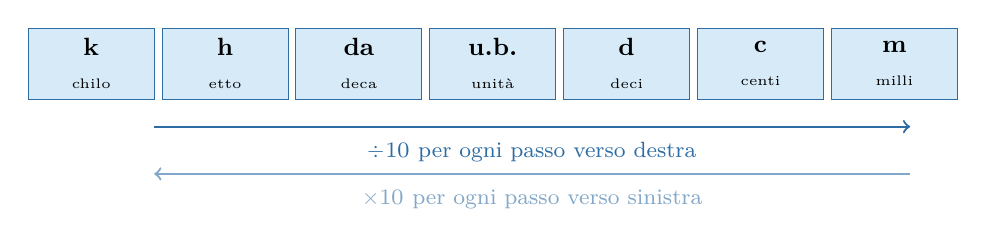
\begin{tikzpicture}[font=\small]
        % Celle della tavola
        \foreach \i/\lbl/\sub in {
                0/k/chilo,
                1/h/etto,
                2/da/deca,
                3/{u.b.}/unità,
                4/d/deci,
                5/c/centi,
                6/m/milli}
            {
                \node[draw=blu, fill=azzurro, minimum width=1.6cm, minimum height=0.9cm,
                    inner sep=2pt, align=center] at (\i*1.7,0.5) {\textbf{\lbl}\\[1pt]\tiny\sub};
            }
        % Frecce
        \draw[->, thick, blu] (0.8,-0.3) -- (10.4,-0.3)
        node[midway, below=2pt]{\footnotesize $\div 10$ per ogni passo verso destra};
        \draw[->, thick, blu!60] (10.4,-0.9) -- (0.8,-0.9)
        node[midway, below=2pt]{\footnotesize $\times 10$ per ogni passo verso sinistra};
    \end{tikzpicture}
\end{center}

\begin{regola}
    Per convertire un'unità in un'unità più piccola (verso destra nella tavola), si \textbf{moltiplica} per una potenza di 10. Per convertire in un'unità più grande (verso sinistra), si \textbf{divide} per una potenza di 10. Il numero di zeri da aggiungere o di cifre da spostare corrisponde al numero di passi effettuati nella tavola.
\end{regola}

% ============================================================
\section{Misure di lunghezza}
% ============================================================

\begin{definizione}
    L'\textbf{unità di misura fondamentale della lunghezza} nel SI è il \textbf{metro} (simbolo: \textbf{m}). La lunghezza esprime la distanza tra due punti.
\end{definizione}

\subsection{Multipli e sottomultipli del metro}

\begin{center}
    \begin{tabular}{lllr}
        \toprule
        \textbf{Nome}  & \textbf{Simbolo} & \textbf{Relazione con il metro}   & \textbf{Valore in m} \\
        \midrule
        chilometro     & km               & $1\,\text{km} = 1000\,\text{m}$   & $1000$               \\
        ettometro      & hm               & $1\,\text{hm} = 100\,\text{m}$    & $100$                \\
        decametro      & dam              & $1\,\text{dam} = 10\,\text{m}$    & $10$                 \\
        \textbf{metro} & \textbf{m}       & \textit{unità base}               & $1$                  \\
        decimetro      & dm               & $1\,\text{dm} = {,}1\,\text{m}$   & ${,}1$               \\
        centimetro     & cm               & $1\,\text{cm} = {,}01\,\text{m}$  & ${,}01$              \\
        millimetro     & mm               & $1\,\text{mm} = {,}001\,\text{m}$ & ${,}001$             \\
        \bottomrule
    \end{tabular}
\end{center}

\begin{esempio}
    \textbf{Conversione di lunghezze}

    \medskip
    \textbf{a)} Convertire $3{,}5\,\text{km}$ in metri.

    Da km a m si fanno \textbf{3 passi verso destra} nella tavola, quindi si moltiplica per $10^3 = 1000$:
    \[
        3{,}5\,\text{km} = 3{,}5 \times 1000\,\text{m} = 3500\,\text{m}
    \]

    \medskip
    \textbf{b)} Convertire $47\,\text{cm}$ in metri.

    Da cm a m si fanno \textbf{2 passi verso sinistra}, quindi si divide per $10^2 = 100$:
    \[
        47\,\text{cm} = 47 \div 100\,\text{m} = {,}47\,\text{m}
    \]

    \medskip
    \textbf{c)} Convertire $2\,\text{km}$ e $340\,\text{m}$ in centimetri.

    Prima si converte tutto in metri: $2\,\text{km} + 340\,\text{m} = 2340\,\text{m}$.\\
    Da m a cm si fanno \textbf{2 passi verso destra}, quindi si moltiplica per $100$:
    \[
        2340\,\text{m} = 2340 \times 100\,\text{cm} = 234\,000\,\text{cm}
    \]
\end{esempio}

\begin{attenzione}
    \textbf{Errore comune — confondere dam e dm.}

    Il \textbf{decametro} (dam) è \emph{dieci volte} il metro; il \textbf{decimetro} (dm) è \emph{un decimo} del metro. I simboli si assomigliano, ma il loro valore è molto diverso: $1\,\text{dam} = 100\,\text{dm}$. Quando si legge un simbolo, occorre verificare se la lettera iniziale è \emph{d} (deci, $\div 10$) oppure \emph{da} (deca, $\times 10$).
\end{attenzione}

% ============================================================
\section{Misure di massa}
% ============================================================

\begin{definizione}
    L'\textbf{unità di misura fondamentale della massa} nel SI è il \textbf{grammo} (simbolo: \textbf{g}). La massa indica la quantità di materia contenuta in un corpo.
\end{definizione}

\begin{attenzione}
    \textbf{Massa e peso non sono la stessa cosa.}

    Nel linguaggio comune si usa spesso la parola \emph{peso} per indicare la massa di un oggetto. In fisica, il \textbf{peso} è la forza con cui la Terra attrae un corpo e dipende dalla gravità; la \textbf{massa} è invece una proprietà intrinseca del corpo e non cambia al variare della gravità. In questo capitolo utilizziamo il termine \emph{massa}, come previsto dal SI.
\end{attenzione}

\subsection{Multipli e sottomultipli del grammo}

\begin{center}
    \begin{tabular}{lllr}
        \toprule
        \textbf{Nome}   & \textbf{Simbolo} & \textbf{Relazione con il grammo}  & \textbf{Valore in g} \\
        \midrule
        chilogrammo     & kg               & $1\,\text{kg} = 1000\,\text{g}$   & $1000$               \\
        ettogrammo      & hg               & $1\,\text{hg} = 100\,\text{g}$    & $100$                \\
        decagrammo      & dag              & $1\,\text{dag} = 10\,\text{g}$    & $10$                 \\
        \textbf{grammo} & \textbf{g}       & \textit{unità base}               & $1$                  \\
        decigrammo      & dg               & $1\,\text{dg} = {,}1\,\text{g}$   & ${,}1$               \\
        centigrammo     & cg               & $1\,\text{cg} = {,}01\,\text{g}$  & ${,}01$              \\
        milligrammo     & mg               & $1\,\text{mg} = {,}001\,\text{g}$ & ${,}001$             \\
        \bottomrule
    \end{tabular}
\end{center}

\begin{sapevi}
    \textbf{La tonnellata}

    Nella vita quotidiana si usa spesso la \textbf{tonnellata} (simbolo: t) per indicare masse molto grandi. Non è un'unità del SI, ma è accettata nell'uso corrente: $1\,\text{t} = 1000\,\text{kg} = 1\,000\,000\,\text{g}$.
\end{sapevi}

\begin{esempio}
    \textbf{Conversione di masse}

    \medskip
    \textbf{a)} Convertire $2\,\text{kg}$ e $350\,\text{g}$ in grammi.

    $1\,\text{kg} = 1000\,\text{g}$, quindi:
    \[
        2\,\text{kg} + 350\,\text{g} = 2000\,\text{g} + 350\,\text{g} = 2350\,\text{g}
    \]

    \medskip
    \textbf{b)} Convertire $4500\,\text{mg}$ in grammi.

    Da mg a g si fanno \textbf{3 passi verso sinistra}, quindi si divide per $1000$:
    \[
        4500\,\text{mg} = 4500 \div 1000\,\text{g} = 4{,}5\,\text{g}
    \]
\end{esempio}

% ============================================================
\section{Misure di capacità}
% ============================================================

\begin{definizione}
    L'\textbf{unità di misura fondamentale della capacità} è il \textbf{litro} (simbolo: \textbf{l} oppure \textbf{L}). La capacità indica il volume di liquido o gas che un contenitore può accogliere.
\end{definizione}

\begin{attenzione}
    \textbf{Il simbolo del litro}

    Il litro si scrive con la lettera elle minuscola (\textbf{l}) o, per evitare confusione con il numero 1, con la lettera \textbf{L} maiuscola. Entrambe le forme sono accettate; in questo libro si usa \textbf{l}.
\end{attenzione}

\subsection{Multipli e sottomultipli del litro}

\begin{center}
    \begin{tabular}{lllr}
        \toprule
        \textbf{Nome}  & \textbf{Simbolo} & \textbf{Relazione con il litro}   & \textbf{Valore in l} \\
        \midrule
        chilolitro     & kl               & $1\,\text{kl} = 1000\,\text{l}$   & $1000$               \\
        ettolitro      & hl               & $1\,\text{hl} = 100\,\text{l}$    & $100$                \\
        decalitro      & dal              & $1\,\text{dal} = 10\,\text{l}$    & $10$                 \\
        \textbf{litro} & \textbf{l}       & \textit{unità base}               & $1$                  \\
        decilitro      & dl               & $1\,\text{dl} = {,}1\,\text{l}$   & ${,}1$               \\
        centilitro     & cl               & $1\,\text{cl} = {,}01\,\text{l}$  & ${,}01$              \\
        millilitro     & ml               & $1\,\text{ml} = {,}001\,\text{l}$ & ${,}001$             \\
        \bottomrule
    \end{tabular}
\end{center}

\begin{esempio}
    \textbf{Conversione di capacità}

    \medskip
    \textbf{a)} Convertire $1{,}5\,\text{l}$ in millilitri.

    Da l a ml si fanno \textbf{3 passi verso destra}, quindi si moltiplica per $1000$:
    \[
        1{,}5\,\text{l} = 1{,}5 \times 1000\,\text{ml} = 1500\,\text{ml}
    \]

    \medskip
    \textbf{b)} Convertire $75\,\text{cl}$ in litri.

    Da cl a l si fanno \textbf{2 passi verso sinistra}, quindi si divide per $100$:
    \[
        75\,\text{cl} = 75 \div 100\,\text{l} = {,}75\,\text{l}
    \]
\end{esempio}

% ============================================================
\section{Misure di superficie}
% ============================================================

\begin{definizione}
    La \textbf{superficie} (o \textbf{area}) misura l'estensione di una figura piana. L'unità di misura fondamentale della superficie nel SI è il \textbf{metro quadrato} (simbolo: \textbf{m\textsuperscript{2}}), che corrisponde all'area di un quadrato con il lato di $1\,\text{m}$.
\end{definizione}

\subsection{Perché si moltiplica per 100 (e non per 10)?}

Passando da un'unità lineare alla corrispondente unità di superficie, il fattore di conversione \textbf{si eleva al quadrato}.

\begin{center}
    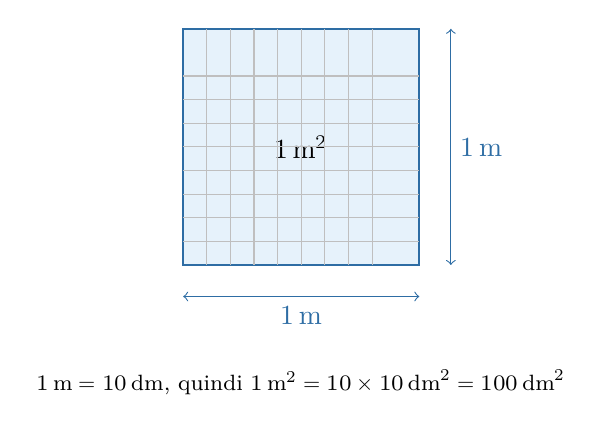
\begin{tikzpicture}
        % Quadrato 1m x 1m
        \draw[thick, blu, fill=azzurro!60] (0,0) rectangle (3,3);
        \node at (1.5,1.5) {$1\,\text{m}^2$};
        \draw[<->, blu] (0,-0.4) -- (3,-0.4) node[midway,below]{$1\,\text{m}$};
        \draw[<->, blu] (3.4,0) -- (3.4,3) node[midway,right]{$1\,\text{m}$};
        % Divisione in dm
        \foreach \x in {0.3,0.6,...,2.7} \draw[gray!50] (\x,0)--(\x,3);
        \foreach \y in {0.3,0.6,...,2.7} \draw[gray!50] (0,\y)--(3,\y);
        \node[below=1.2cm] at (1.5,0) {\footnotesize $1\,\text{m} = 10\,\text{dm}$, quindi $1\,\text{m}^2 = 10 \times 10\,\text{dm}^2 = 100\,\text{dm}^2$};
    \end{tikzpicture}
\end{center}

\begin{regola}
    Tra unità di superficie consecutive nella tavola, il fattore di conversione è $\mathbf{100}$ (non 10), perché la superficie ha \textbf{due dimensioni}.

    \[
        1\,\text{m}^2 = 100\,\text{dm}^2 \qquad 1\,\text{dm}^2 = 100\,\text{cm}^2 \qquad 1\,\text{cm}^2 = 100\,\text{mm}^2
    \]

    Per passare a un'unità più piccola si moltiplica per $100$; per passare a un'unità più grande si divide per $100$.
\end{regola}

\subsection{Tavola delle misure di superficie}

\begin{center}
    \begin{tabular}{lllr}
        \toprule
        \textbf{Nome}           & \textbf{Simbolo}              & \textbf{Relazione}                         & \textbf{Valore in m\textsuperscript{2}} \\
        \midrule
        chilometro quadrato     & km\textsuperscript{2}         & $1\,\text{km}^2 = 1\,000\,000\,\text{m}^2$ & $1\,000\,000$                           \\
        ettometro quadrato      & hm\textsuperscript{2}         & $1\,\text{hm}^2 = 10\,000\,\text{m}^2$     & $10\,000$                               \\
        decametro quadrato      & dam\textsuperscript{2}        & $1\,\text{dam}^2 = 100\,\text{m}^2$        & $100$                                   \\
        \textbf{metro quadrato} & \textbf{m\textsuperscript{2}} & \textit{unità base}                        & $1$                                     \\
        decimetro quadrato      & dm\textsuperscript{2}         & $1\,\text{dm}^2 = 0{,}01\,\text{m}^2$      & ${,}01$                                 \\
        centimetro quadrato     & cm\textsuperscript{2}         & $1\,\text{cm}^2 = 0{,}0001\,\text{m}^2$    & ${,}0001$                               \\
        millimetro quadrato     & mm\textsuperscript{2}         & $1\,\text{mm}^2 = 0{,}000001\,\text{m}^2$  & ${,}000001$                             \\
        \bottomrule
    \end{tabular}
\end{center}

\begin{esempio}
    \textbf{Conversione di superfici}

    \medskip
    \textbf{a)} Convertire $3\,\text{m}^2$ in centimetri quadrati.

    Da m\textsuperscript{2} a cm\textsuperscript{2} ci sono \textbf{2 passi} nella tavola delle superfici, quindi si moltiplica per $100^2 = 10\,000$:
    \[
        3\,\text{m}^2 = 3 \times 10\,000\,\text{cm}^2 = 30\,000\,\text{cm}^2
    \]

    \medskip
    \textbf{b)} Convertire $450\,\text{dm}^2$ in metri quadrati.

    Da dm\textsuperscript{2} a m\textsuperscript{2} c'è \textbf{1 passo verso sinistra}, quindi si divide per $100$:
    \[
        450\,\text{dm}^2 = 450 \div 100\,\text{m}^2 = 4{,}5\,\text{m}^2
    \]
\end{esempio}

\begin{attenzione}
    \textbf{Errore comune — applicare il fattore lineare alle superfici.}

    Un errore frequente è dividere o moltiplicare per $10$ invece che per $100$ quando si convertono superfici. Ricordare sempre: le superfici hanno due dimensioni, quindi il fattore di conversione è $10^2 = 100$ per ogni passo nella tavola. Ad esempio, $1\,\text{m}^2 \neq 10\,\text{dm}^2$, ma $1\,\text{m}^2 = 100\,\text{dm}^2$.
\end{attenzione}

% ============================================================
\section{Misure di volume}
% ============================================================

\begin{definizione}
    Il \textbf{volume} misura lo spazio occupato da un corpo nello spazio tridimensionale. L'unità di misura fondamentale del volume nel SI è il \textbf{metro cubo} (simbolo: \textbf{m\textsuperscript{3}}), che corrisponde al volume di un cubo con spigolo di $1\,\text{m}$.
\end{definizione}

\subsection{Perché si moltiplica per 1000?}

Passando da un'unità lineare alla corrispondente unità di volume, il fattore di conversione \textbf{si eleva al cubo}.

\begin{center}
    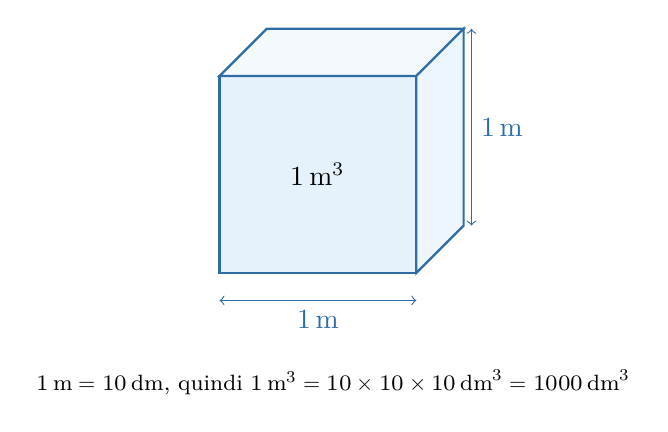
\begin{tikzpicture}
        % Cubo stilizzato in assonometria
        \def\a{2.5}
        \def\s{0.6}
        % Faccia frontale
        \draw[thick, blu, fill=azzurro!60] (0,0) rectangle (\a,\a);
        % Faccia superiore
        \draw[thick, blu, fill=azzurro!30]
        (0,\a) -- (\s,\a+\s) -- (\a+\s,\a+\s) -- (\a,\a) -- cycle;
        % Faccia laterale destra
        \draw[thick, blu, fill=azzurro!45]
        (\a,0) -- (\a+\s,\s) -- (\a+\s,\a+\s) -- (\a,\a) -- cycle;
        % Quote
        \draw[<->, blu] (0,-0.35) -- (\a,-0.35) node[midway,below]{$1\,\text{m}$};
        \draw[<->, blu] (\a+\s+0.1,\s) -- (\a+\s+0.1,\a+\s) node[midway,right]{$1\,\text{m}$};
        \node at (\a/2, \a/2) {$1\,\text{m}^3$};
        \node[below=1.1cm] at (\a/2+0.2,0)
        {\footnotesize $1\,\text{m} = 10\,\text{dm}$, quindi $1\,\text{m}^3 = 10 \times 10 \times 10\,\text{dm}^3 = 1000\,\text{dm}^3$};
    \end{tikzpicture}
\end{center}

\begin{regola}
    Tra unità di volume consecutive nella tavola, il fattore di conversione è $\mathbf{1000}$, perché il volume ha \textbf{tre dimensioni}.

    \[
        1\,\text{m}^3 = 1000\,\text{dm}^3 \qquad 1\,\text{dm}^3 = 1000\,\text{cm}^3 \qquad 1\,\text{cm}^3 = 1000\,\text{mm}^3
    \]

    Per passare a un'unità più piccola si moltiplica per $1000$; per passare a un'unità più grande si divide per $1000$.
\end{regola}

\subsection{Tavola delle misure di volume}

\begin{center}
    \begin{tabular}{lllr}
        \toprule
        \textbf{Nome}       & \textbf{Simbolo}              & \textbf{Relazione}                        & \textbf{Valore in m\textsuperscript{3}} \\
        \midrule
        chilometro cubo     & km\textsuperscript{3}         & $1\,\text{km}^3 = 10^9\,\text{m}^3$       & $1\,000\,000\,000$                      \\
        ettometro cubo      & hm\textsuperscript{3}         & $1\,\text{hm}^3 = 10^6\,\text{m}^3$       & $1\,000\,000$                           \\
        decametro cubo      & dam\textsuperscript{3}        & $1\,\text{dam}^3 = 1000\,\text{m}^3$      & $1\,000$                                \\
        \textbf{metro cubo} & \textbf{m\textsuperscript{3}} & \textit{unità base}                       & $1$                                     \\
        decimetro cubo      & dm\textsuperscript{3}         & $1\,\text{dm}^3 = 0{,}001\,\text{m}^3$    & ${,}001$                                \\
        centimetro cubo     & cm\textsuperscript{3}         & $1\,\text{cm}^3 = 0{,}000001\,\text{m}^3$ & ${,}000001$                             \\
        millimetro cubo     & mm\textsuperscript{3}         & $1\,\text{mm}^3 = 10^{-9}\,\text{m}^3$    & ${,}000000001$                          \\
        \bottomrule
    \end{tabular}
\end{center}

\begin{esempio}
    \textbf{Conversione di volumi}

    \medskip
    \textbf{a)} Convertire $2\,\text{m}^3$ in decimetri cubi.

    Da m\textsuperscript{3} a dm\textsuperscript{3} c'è \textbf{1 passo verso destra}, quindi si moltiplica per $1000$:
    \[
        2\,\text{m}^3 = 2 \times 1000\,\text{dm}^3 = 2000\,\text{dm}^3
    \]

    \medskip
    \textbf{b)} Convertire $5\,\text{dm}^3$ in centimetri cubi.

    Da dm\textsuperscript{3} a cm\textsuperscript{3} c'è \textbf{1 passo verso destra}, quindi si moltiplica per $1000$:
    \[
        5\,\text{dm}^3 = 5 \times 1000\,\text{cm}^3 = 5000\,\text{cm}^3
    \]
\end{esempio}

\begin{attenzione}
    \textbf{Errore comune — applicare il fattore lineare o quadratico ai volumi.}

    Per i volumi il fattore per ogni passo è $10^3 = 1000$, non $10$ né $100$. Questo vale per ogni coppia di unità adiacenti: $1\,\text{dm}^3 = 1000\,\text{cm}^3$, non $100\,\text{cm}^3$.
\end{attenzione}

% ============================================================
\section{Relazione tra decimetro cubo e litro}
% ============================================================

\begin{definizione}
    Il \textbf{decimetro cubo} e il \textbf{litro} sono due unità di misura equivalenti:
    \[
        \boxed{1\,\text{dm}^3 = 1\,\text{l}}
    \]
    In modo analogo: $1\,\text{cm}^3 = 1\,\text{ml}$ e $1\,\text{m}^3 = 1000\,\text{l}$.
\end{definizione}

Questa relazione deriva dalla definizione storica del litro: il litro fu definito come il volume occupato da un chilogrammo di acqua pura a $4\,°\text{C}$, che corrisponde esattamente a un decimetro cubo.

\begin{center}
    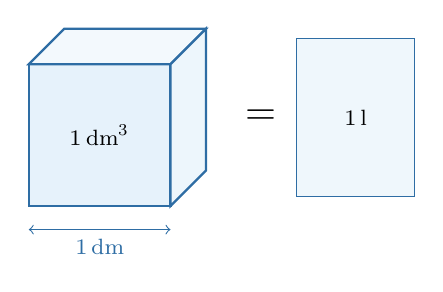
\begin{tikzpicture}
        % Cubo dm
        \def\a{1.8}
        \def\s{0.45}
        \draw[thick, blu, fill=azzurro!60] (0,0) rectangle (\a,\a);
        \draw[thick, blu, fill=azzurro!30]
        (0,\a) -- (\s,\a+\s) -- (\a+\s,\a+\s) -- (\a,\a) -- cycle;
        \draw[thick, blu, fill=azzurro!45]
        (\a,0) -- (\a+\s,\s) -- (\a+\s,\a+\s) -- (\a,\a) -- cycle;
        \draw[<->, blu] (0,-0.3) -- (\a,-0.3) node[midway,below]{\footnotesize $1\,\text{dm}$};
        \node at (\a/2,\a/2) {\footnotesize $1\,\text{dm}^3$};
        % Simbolo uguale
        \node at (\a+\s+0.7,\a/2+\s/2) {\Large $=$};
        % Etichetta litro
        \node[draw=blu, fill=azzurro!40, minimum width=1.5cm, minimum height=\a cm+0.2cm,
            inner sep=4pt, align=center] at (\a+\s+1.9,\a/2+\s/2)
        {\footnotesize $1\,\text{l}$};
    \end{tikzpicture}
\end{center}

\begin{regola}
    Grazie alla relazione $1\,\text{dm}^3 = 1\,\text{l}$, è possibile convertire direttamente tra misure di volume e misure di capacità:
    \[
        1\,\text{m}^3 = 1000\,\text{l} \qquad\qquad 1\,\text{cm}^3 = 1\,\text{ml}
    \]
\end{regola}

\begin{esempio}
    \textbf{Conversione tra volume e capacità}

    \medskip
    \textbf{a)} Una vasca da bagno ha un volume di ${,}3\,\text{m}^3$. Quanti litri contiene?

    $1\,\text{m}^3 = 1000\,\text{l}$, quindi:
    \[
        {,}3\,\text{m}^3 = 0{,}3 \times 1000\,\text{l} = 300\,\text{l}
    \]

    \medskip
    \textbf{b)} Una bottiglia contiene $750\,\text{ml}$. Qual è il suo volume in centimetri cubi?

    $1\,\text{ml} = 1\,\text{cm}^3$, quindi:
    \[
        750\,\text{ml} = 750\,\text{cm}^3
    \]
\end{esempio}

\begin{sapevi}
    \textbf{Perché l'acqua è lo standard?}

    Nell'antichità le misure variavano da città a città. Nel 1795, dopo la Rivoluzione Francese, la Francia introdusse il sistema metrico per unificare le misure in tutto il Paese. Il litro fu definito in riferimento all'acqua proprio perché è una sostanza facilmente disponibile ovunque e con proprietà fisiche precise e riproducibili.
\end{sapevi}

% ============================================================
\section{Misure agrarie}
% ============================================================

\begin{definizione}
    Le \textbf{misure agrarie} sono unità di misura della superficie utilizzate tradizionalmente per indicare l'estensione di terreni agricoli. Le principali sono:
    \begin{itemize}[noitemsep]
        \item l'\textbf{ara} (simbolo: \textbf{a}), pari a $1\,\text{dam}^2 = 100\,\text{m}^2$;
        \item l'\textbf{ettaro} (simbolo: \textbf{ha}), pari a $1\,\text{hm}^2 = 10\,000\,\text{m}^2$.
    \end{itemize}
\end{definizione}

\begin{center}
    \begin{tabular}{llr}
        \toprule
        \textbf{Unità}                                                                            & \textbf{Equivalenza}            & \textbf{Valore in m\textsuperscript{2}} \\
        \midrule
        ettaro (ha)                                                                               & $1\,\text{ha} = 100\,\text{a}$  & $10\,000$                               \\
        ara (a)                                                                                   & $1\,\text{a} = 100\,\text{m}^2$ & $100$                                   \\
        \midrule
        \multicolumn{2}{l}{$1\,\text{ha} = 100\,\text{a} = 10\,000\,\text{m}^2 = 1\,\text{hm}^2$} &                                                                           \\
        \bottomrule
    \end{tabular}
\end{center}

\begin{regola}
    \[
        1\,\text{ha} = 100\,\text{a} \qquad 1\,\text{a} = 100\,\text{m}^2 \qquad 1\,\text{ha} = 10\,000\,\text{m}^2
    \]
\end{regola}

\begin{esempio}
    \textbf{Conversione con misure agrarie}

    \medskip
    \textbf{a)} Un campo ha un'estensione di $3{,}5\,\text{ha}$. Quanti metri quadrati sono?

    $1\,\text{ha} = 10\,000\,\text{m}^2$, quindi:
    \[
        3{,}5\,\text{ha} = 3{,}5 \times 10\,000\,\text{m}^2 = 35\,000\,\text{m}^2
    \]

    \medskip
    \textbf{b)} Un terreno misura $2500\,\text{m}^2$. Quante are sono?

    $1\,\text{a} = 100\,\text{m}^2$, quindi:
    \[
        2500\,\text{m}^2 = 2500 \div 100\,\text{a} = 25\,\text{a}
    \]
\end{esempio}

\begin{sapevi}
    \textbf{L'ettaro nella vita quotidiana}

    L'ettaro è tuttora l'unità più usata in agricoltura e nel settore immobiliare per i terreni. In Svizzera, i dati sulla superficie agricola sono sistematicamente espressi in ettari. Un campo da calcio standard ha un'area di circa ${,}7\,\text{ha}$.
\end{sapevi}

% ============================================================
\section{Riepilogo}
% ============================================================

\begin{regola}
    \textbf{Riepilogo delle conversioni fondamentali}

    \medskip
    \textbf{Misure lineari} — fattore $\times 10$ per ogni passo verso destra (unità più piccola):
    \[
        1\,\text{km} = 10\,\text{hm} = 100\,\text{dam} = 1000\,\text{m} = 10\,000\,\text{dm} = 100\,000\,\text{cm} = 1\,000\,000\,\text{mm}
    \]

    \medskip
    \textbf{Misure di massa} — fattore $\times 10$ per ogni passo:
    \[
        1\,\text{kg} = 10\,\text{hg} = 100\,\text{dag} = 1000\,\text{g} = 10\,000\,\text{dg} = 100\,000\,\text{cg} = 1\,000\,000\,\text{mg}
    \]

    \medskip
    \textbf{Misure di capacità} — fattore $\times 10$ per ogni passo:
    \[
        1\,\text{kl} = 10\,\text{hl} = 100\,\text{dal} = 1000\,\text{l} = 10\,000\,\text{dl} = 100\,000\,\text{cl} = 1\,000\,000\,\text{ml}
    \]

    \medskip
    \textbf{Misure di superficie} — fattore $\times 100$ per ogni passo:
    \[
        1\,\text{km}^2 = 100\,\text{hm}^2 = 10\,000\,\text{dam}^2 = \ldots
    \]

    \medskip
    \textbf{Misure di volume} — fattore $\times 1000$ per ogni passo:
    \[
        1\,\text{m}^3 = 1000\,\text{dm}^3 = 1\,000\,000\,\text{cm}^3 = 1\,000\,000\,000\,\text{mm}^3
    \]

    \medskip
    \textbf{Relazione volume–capacità}:
    \[
        1\,\text{dm}^3 = 1\,\text{l} \qquad 1\,\text{cm}^3 = 1\,\text{ml} \qquad 1\,\text{m}^3 = 1000\,\text{l}
    \]

    \medskip
    \textbf{Misure agrarie}:
    \[
        1\,\text{ha} = 100\,\text{a} = 10\,000\,\text{m}^2
    \]
\end{regola}

% ============================================================
%  Capitolo — Geometria piana
%  Matemagica — Scuole medie Canton Ticino (DECS)
% ============================================================

\chapter{Geometria piana}

% --- Obiettivi di apprendimento ------------------------------
\section*{Obiettivi di apprendimento}
\begin{itemize}[leftmargin=1.5em]
    \item Comprendere il significato di figura piana, perimetro e area.
    \item Conoscere le principali figure piane: quadrato, rettangolo, triangolo, trapezio, rombo e parallelogramma.
    \item Calcolare il perimetro e l'area di ciascuna figura.
    \item Riconoscere le relazioni tra le diverse figure piane.
\end{itemize}

% =============================================================
\section{Che cos'è la geometria piana}
% =============================================================

\begin{definizione}
    La \textbf{geometria piana} è la parte della matematica che studia le figure che si trovano su un piano, cioè su una superficie piatta e illimitata. Le figure piane sono delimitate da lati (segmenti) o curve e non hanno spessore.
\end{definizione}

Le figure piane più importanti sono i \textbf{poligoni}: figure chiuse i cui lati sono tutti segmenti. In questo capitolo studieremo i poligoni più comuni: quadrato, rettangolo, triangolo, trapezio, rombo e parallelogramma.

% =============================================================
\section{Perimetro e area}
% =============================================================

\begin{definizione}
    Il \textbf{perimetro} di una figura piana è la lunghezza totale del suo contorno, cioè la somma delle lunghezze di tutti i suoi lati. Si misura in unità di lunghezza (cm, m, km, \ldots).
\end{definizione}

\begin{definizione}
    L'\textbf{area} di una figura piana è la misura della superficie racchiusa dalla figura. Si misura in unità di superficie (cm\textsuperscript{2}, m\textsuperscript{2}, km\textsuperscript{2}, \ldots).
\end{definizione}

\begin{attenzione}
    \textbf{Attenzione:} perimetro e area sono due misure diverse. Il perimetro misura quanto è lungo il bordo della figura; l'area misura quanto è grande la sua superficie. Due figure con lo stesso perimetro possono avere aree diverse, e viceversa.
\end{attenzione}

% =============================================================
\section{Il quadrato}
% =============================================================

\subsection{Definizione}

\begin{definizione}
    Il \textbf{quadrato} è un poligono con quattro lati uguali e quattro angoli retti (di 90°). È un caso particolare sia di rettangolo sia di rombo.
\end{definizione}

\begin{center}
    \begin{tikzpicture}
        \draw[thick, color=blu] (0,0) rectangle (2.5,2.5);
        % angoli retti
        \draw[blu] (0.25,0) -- (0.25,0.25) -- (0,0.25);
        \draw[blu] (2.25,0) -- (2.25,0.25) -- (2.5,0.25);
        \draw[blu] (0.25,2.5) -- (0.25,2.25) -- (0,2.25);
        \draw[blu] (2.25,2.5) -- (2.25,2.25) -- (2.5,2.25);
        % etichette lati
        \node[below] at (1.25,0) {$l$};
        \node[right] at (2.5,1.25) {$l$};
        \node[above] at (1.25,2.5) {$l$};
        \node[left]  at (0,1.25)  {$l$};
    \end{tikzpicture}
\end{center}

\subsection{Perimetro}

\begin{regola}
    Il \textbf{perimetro del quadrato} si calcola moltiplicando la lunghezza del lato per 4:
    \[
        P = 4 \times l
    \]
    dove $l$ è la lunghezza del lato.
\end{regola}

\begin{esempio}
    Un quadrato ha il lato di 6 cm. Calcola il suo perimetro.

    \medskip
    \textbf{Dati:} $l = 6$ cm

    \textbf{Formula:} $P = 4 \times l$

    \textbf{Calcolo:} $P = 4 \times 6 = 24$ cm

    \textbf{Risposta:} Il perimetro del quadrato è \textbf{24 cm}.
\end{esempio}

\subsection{Area}

\begin{regola}
    L'\textbf{area del quadrato} si calcola elevando al quadrato la lunghezza del lato:
    \[
        A = l \times l = l^2
    \]
    dove $l$ è la lunghezza del lato.
\end{regola}

\begin{esempio}
    Un quadrato ha il lato di 6 cm. Calcola la sua area.

    \medskip
    \textbf{Dati:} $l = 6$ cm

    \textbf{Formula:} $A = l^2$

    \textbf{Calcolo:} $A = 6^2 = 36$ cm\textsuperscript{2}

    \textbf{Risposta:} L'area del quadrato è \textbf{36 cm\textsuperscript{2}}.
\end{esempio}

% =============================================================
\section{Il rettangolo}
% =============================================================

\subsection{Definizione}

\begin{definizione}
    Il \textbf{rettangolo} è un poligono con quattro angoli retti (di 90°) e lati opposti uguali e paralleli. I due lati diversi si chiamano \textbf{base} ($b$) e \textbf{altezza} ($h$). Il quadrato è un caso particolare di rettangolo in cui base e altezza sono uguali.
\end{definizione}

\begin{center}
    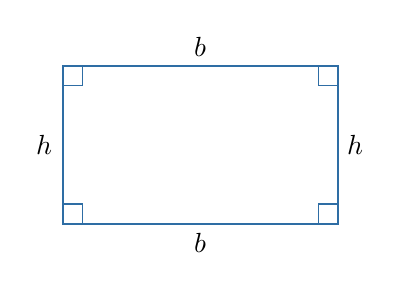
\begin{tikzpicture}
        \draw[thick, color=blu] (0,0) rectangle (3.5,2);
        \draw[blu] (0.25,0) -- (0.25,0.25) -- (0,0.25);
        \draw[blu] (3.25,0) -- (3.25,0.25) -- (3.5,0.25);
        \draw[blu] (0.25,2) -- (0.25,1.75) -- (0,1.75);
        \draw[blu] (3.25,2) -- (3.25,1.75) -- (3.5,1.75);
        \node[below] at (1.75,0) {$b$};
        \node[right] at (3.5,1)  {$h$};
        \node[above] at (1.75,2) {$b$};
        \node[left]  at (0,1)    {$h$};
    \end{tikzpicture}
\end{center}

\subsection{Perimetro}

\begin{regola}
    Il \textbf{perimetro del rettangolo} è la somma di tutti i lati, cioè il doppio della somma di base e altezza:
    \[
        P = 2 \times (b + h)
    \]
    dove $b$ è la base e $h$ è l'altezza.
\end{regola}

\begin{esempio}
    Un rettangolo ha base 8 cm e altezza 3 cm. Calcola il perimetro.

    \medskip
    \textbf{Dati:} $b = 8$ cm, $h = 3$ cm

    \textbf{Formula:} $P = 2 \times (b + h)$

    \textbf{Calcolo:} $P = 2 \times (8 + 3) = 2 \times 11 = 22$ cm

    \textbf{Risposta:} Il perimetro del rettangolo è \textbf{22 cm}.
\end{esempio}

\subsection{Area}

\begin{regola}
    L'\textbf{area del rettangolo} si calcola moltiplicando la base per l'altezza:
    \[
        A = b \times h
    \]
\end{regola}

\begin{esempio}
    Un rettangolo ha base 8 cm e altezza 3 cm. Calcola l'area.

    \medskip
    \textbf{Dati:} $b = 8$ cm, $h = 3$ cm

    \textbf{Formula:} $A = b \times h$

    \textbf{Calcolo:} $A = 8 \times 3 = 24$ cm\textsuperscript{2}

    \textbf{Risposta:} L'area del rettangolo è \textbf{24 cm\textsuperscript{2}}.
\end{esempio}

% =============================================================
\section{Il triangolo}
% =============================================================

\subsection{Definizione}

\begin{definizione}
    Il \textbf{triangolo} è un poligono con tre lati e tre angoli. La somma dei tre angoli interni di qualsiasi triangolo è sempre uguale a 180°.
\end{definizione}

I triangoli si classificano in due modi: in base ai \textbf{lati} e in base agli \textbf{angoli}.

\subsubsection*{Classificazione in base ai lati}

\begin{itemize}[leftmargin=1.5em]
    \item \textbf{Scaleno}: tutti e tre i lati hanno lunghezze diverse.
    \item \textbf{Isoscele}: due lati (detti \textbf{lati obliqui}) sono uguali; il terzo si chiama \textbf{base}.
    \item \textbf{Equilatero}: tutti e tre i lati sono uguali. Tutti e tre gli angoli misurano 60°.
\end{itemize}

\subsubsection*{Classificazione in base agli angoli}

\begin{itemize}[leftmargin=1.5em]
    \item \textbf{Acutangolo}: tutti e tre gli angoli sono acuti (minori di 90°).
    \item \textbf{Rettangolo}: ha un angolo retto (di 90°). I due lati che formano l'angolo retto si chiamano \textbf{cateti}; il lato opposto si chiama \textbf{ipotenusa}.
    \item \textbf{Ottusangolo}: ha un angolo ottuso (maggiore di 90°).
\end{itemize}

\begin{center}
    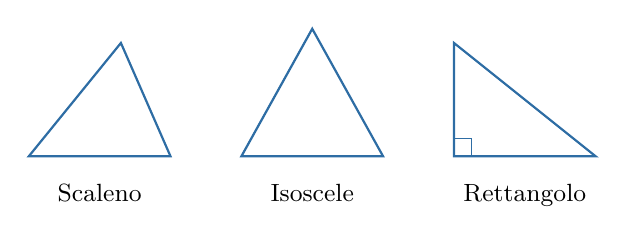
\begin{tikzpicture}[scale=0.9]
        % Scaleno
        \draw[thick, color=blu] (0,0) -- (2,0) -- (1.3,1.6) -- cycle;
        \node[below] at (1,-0.25) {\small Scaleno};
        % Isoscele
        \draw[thick, color=blu] (3,0) -- (5,0) -- (4,1.8) -- cycle;
        \node[below] at (4,-0.25) {\small Isoscele};
        % Rettangolo
        \draw[thick, color=blu] (6,0) -- (8,0) -- (6,1.6) -- cycle;
        \draw[blu] (6.25,0) -- (6.25,0.25) -- (6,0.25);
        \node[below] at (7,-0.25) {\small Rettangolo};
    \end{tikzpicture}
\end{center}

\subsubsection*{Altezza di un triangolo}

\begin{definizione}
    L'\textbf{altezza} di un triangolo relativa a un lato (detto \textbf{base}) è il segmento perpendicolare condotto da un vertice opposto a quella base (o alla sua estensione). Ogni triangolo ha tre altezze, una per ciascun lato scelto come base.
\end{definizione}

\begin{center}
    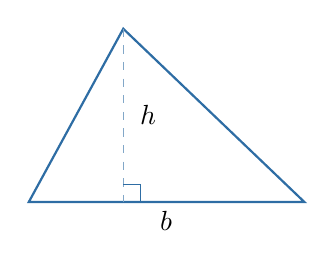
\begin{tikzpicture}
        \coordinate (A) at (0,0);
        \coordinate (B) at (3.5,0);
        \coordinate (C) at (1.2,2.2);
        \draw[thick, color=blu] (A) -- (B) -- (C) -- cycle;
        % piede dell'altezza
        \coordinate (H) at (1.2,0);
        \draw[dashed, color=blu!60] (C) -- (H);
        \draw[blu] (1.2,0.22) -- (1.42,0.22) -- (1.42,0);
        \node[below] at (1.75,0) {$b$};
        \node[right]  at (1.3,1.1) {$h$};
    \end{tikzpicture}
\end{center}

\subsection{Perimetro}

\begin{regola}
    Il \textbf{perimetro del triangolo} è la somma delle lunghezze dei tre lati:
    \[
        P = a + b + c
    \]
    dove $a$, $b$, $c$ sono i tre lati.
\end{regola}

\begin{esempio}
    Un triangolo ha lati di 5 cm, 7 cm e 9 cm. Calcola il perimetro.

    \medskip
    \textbf{Dati:} $a = 5$ cm, $b = 7$ cm, $c = 9$ cm

    \textbf{Formula:} $P = a + b + c$

    \textbf{Calcolo:} $P = 5 + 7 + 9 = 21$ cm

    \textbf{Risposta:} Il perimetro del triangolo è \textbf{21 cm}.
\end{esempio}

\subsection{Area}

\begin{regola}
    L'\textbf{area del triangolo} si calcola moltiplicando la base per l'altezza corrispondente e dividendo per 2:
    \[
        A = \frac{b \times h}{2}
    \]
    dove $b$ è la base scelta e $h$ è l'altezza relativa a quella base.
\end{regola}

\begin{attenzione}
    \textbf{Attenzione:} la base e l'altezza devono essere \textbf{perpendicolari} tra loro. Non si può moltiplicare due lati qualsiasi: l'altezza non è un lato, ma un segmento perpendicolare alla base.
\end{attenzione}

\begin{esempio}
    Un triangolo ha base 10 cm e altezza 6 cm. Calcola l'area.

    \medskip
    \textbf{Dati:} $b = 10$ cm, $h = 6$ cm

    \textbf{Formula:} $A = \dfrac{b \times h}{2}$

    \textbf{Calcolo:} $A = \dfrac{10 \times 6}{2} = \dfrac{60}{2} = 30$ cm\textsuperscript{2}

    \textbf{Risposta:} L'area del triangolo è \textbf{30 cm\textsuperscript{2}}.
\end{esempio}

\begin{sapevi}
    \textbf{Lo sapevi?} La formula dell'area del triangolo si ricava dal rettangolo: se si raddoppia un triangolo (facendone una copia capovolta e attaccandola), si ottiene sempre un parallelogramma o un rettangolo. L'area del triangolo è quindi esattamente la metà di quella figura.
\end{sapevi}

% =============================================================
\section{Il trapezio}
% =============================================================

\subsection{Definizione}

\begin{definizione}
    Il \textbf{trapezio} è un quadrilatero con esattamente una coppia di lati paralleli, chiamati \textbf{basi}: la \textbf{base maggiore} ($B$) e la \textbf{base minore} ($b$). I due lati non paralleli si chiamano \textbf{lati obliqui}. L'\textbf{altezza} ($h$) è la distanza perpendicolare tra le due basi.
\end{definizione}

I tipi di trapezio più comuni sono:
\begin{itemize}[leftmargin=1.5em]
    \item \textbf{Trapezio scaleno}: i due lati obliqui hanno lunghezze diverse.
    \item \textbf{Trapezio isoscele}: i due lati obliqui sono uguali. Gli angoli adiacenti a ciascuna base sono uguali tra loro.
    \item \textbf{Trapezio rettangolo}: uno dei lati obliqui è perpendicolare alle basi (forma un angolo retto con esse).
\end{itemize}

\begin{center}
    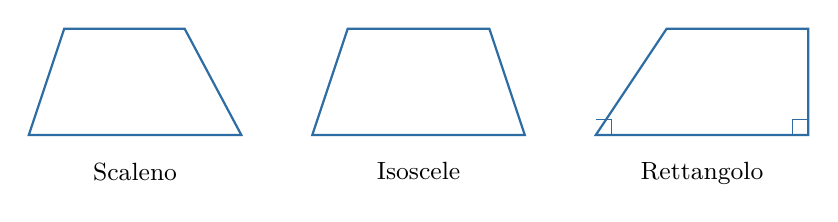
\begin{tikzpicture}[scale=0.9]
        % Trapezio scaleno
        \draw[thick, color=blu] (0,0) -- (3,0) -- (2.2,1.5) -- (0.5,1.5) -- cycle;
        \node[below] at (1.5,-0.25) {\small Scaleno};
        % Trapezio isoscele
        \draw[thick, color=blu] (4,0) -- (7,0) -- (6.5,1.5) -- (4.5,1.5) -- cycle;
        \node[below] at (5.5,-0.25) {\small Isoscele};
        % Trapezio rettangolo
        \draw[thick, color=blu] (8,0) -- (11,0) -- (11,1.5) -- (9,1.5) -- cycle;
        \draw[blu] (8.22,0) -- (8.22,0.22) -- (8,0.22);
        \draw[blu] (10.78,0) -- (10.78,0.22) -- (11,0.22);
        \node[below] at (9.5,-0.25) {\small Rettangolo};
    \end{tikzpicture}
\end{center}

\subsection{Perimetro}

\begin{regola}
    Il \textbf{perimetro del trapezio} è la somma dei quattro lati:
    \[
        P = B + b + c + d
    \]
    dove $B$ è la base maggiore, $b$ la base minore, $c$ e $d$ i lati obliqui.
\end{regola}

\begin{esempio}
    Un trapezio ha base maggiore 12 cm, base minore 6 cm e lati obliqui di 5 cm e 7 cm. Calcola il perimetro.

    \medskip
    \textbf{Dati:} $B = 12$ cm, $b = 6$ cm, $c = 5$ cm, $d = 7$ cm

    \textbf{Formula:} $P = B + b + c + d$

    \textbf{Calcolo:} $P = 12 + 6 + 5 + 7 = 30$ cm

    \textbf{Risposta:} Il perimetro del trapezio è \textbf{30 cm}.
\end{esempio}

\subsection{Area}

\begin{regola}
    L'\textbf{area del trapezio} si calcola moltiplicando la somma delle due basi per l'altezza e dividendo per 2:
    \[
        A = \frac{(B + b) \times h}{2}
    \]
    dove $B$ è la base maggiore, $b$ la base minore e $h$ l'altezza.
\end{regola}

\begin{esempio}
    Un trapezio ha base maggiore 10 cm, base minore 4 cm e altezza 5 cm. Calcola l'area.

    \medskip
    \textbf{Dati:} $B = 10$ cm, $b = 4$ cm, $h = 5$ cm

    \textbf{Formula:} $A = \dfrac{(B + b) \times h}{2}$

    \textbf{Calcolo:} $A = \dfrac{(10 + 4) \times 5}{2} = \dfrac{14 \times 5}{2} = \dfrac{70}{2} = 35$ cm\textsuperscript{2}

    \textbf{Risposta:} L'area del trapezio è \textbf{35 cm\textsuperscript{2}}.
\end{esempio}

% =============================================================
\section{Il rombo}
% =============================================================

\subsection{Definizione}

\begin{definizione}
    Il \textbf{rombo} è un parallelogramma con tutti e quattro i lati uguali. Le sue \textbf{diagonali} (i segmenti che uniscono i vertici opposti) si intersecano perpendicolarmente nel loro punto medio e hanno lunghezze diverse (chiamate \textbf{diagonale maggiore} $d_1$ e \textbf{diagonale minore} $d_2$). Il quadrato è un caso particolare di rombo in cui le due diagonali sono uguali.
\end{definizione}

\begin{center}
    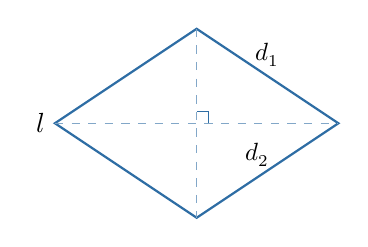
\begin{tikzpicture}
        \coordinate (L) at (0,1.2);
        \coordinate (T) at (1.8,2.4);
        \coordinate (R) at (3.6,1.2);
        \coordinate (Bo) at (1.8,0);
        \draw[thick, color=blu] (L) -- (T) -- (R) -- (Bo) -- cycle;
        % diagonali
        \draw[dashed, color=blu!60] (L) -- (R);
        \draw[dashed, color=blu!60] (T) -- (Bo);
        % simbolo perpendicolarità
        \draw[blu] (1.8,1.2) ++(0.15,0) -- ++(0,0.15) -- ++(-0.15,0);
        % etichette
        \node[above] at (2.7,1.8) {\small $d_1$};
        \node[right] at (2.3,0.8) {\small $d_2$};
        \node[left]  at (0,1.2)   {$l$};
    \end{tikzpicture}
\end{center}

\subsection{Perimetro}

\begin{regola}
    Il \textbf{perimetro del rombo} si calcola moltiplicando la lunghezza del lato per 4 (come per il quadrato, poiché tutti i lati sono uguali):
    \[
        P = 4 \times l
    \]
\end{regola}

\begin{esempio}
    Un rombo ha il lato di 9 cm. Calcola il perimetro.

    \medskip
    \textbf{Dati:} $l = 9$ cm

    \textbf{Formula:} $P = 4 \times l$

    \textbf{Calcolo:} $P = 4 \times 9 = 36$ cm

    \textbf{Risposta:} Il perimetro del rombo è \textbf{36 cm}.
\end{esempio}

\subsection{Area}

\begin{regola}
    L'\textbf{area del rombo} si calcola moltiplicando le due diagonali e dividendo per 2:
    \[
        A = \frac{d_1 \times d_2}{2}
    \]
    dove $d_1$ e $d_2$ sono le due diagonali.
\end{regola}

\begin{attenzione}
    \textbf{Attenzione:} per calcolare l'area del rombo si usano le \textbf{diagonali}, non i lati. Questo è diverso dal quadrato, dove si usa il lato. Non confondere le due formule.
\end{attenzione}

\begin{esempio}
    Un rombo ha diagonale maggiore 12 cm e diagonale minore 8 cm. Calcola l'area.

    \medskip
    \textbf{Dati:} $d_1 = 12$ cm, $d_2 = 8$ cm

    \textbf{Formula:} $A = \dfrac{d_1 \times d_2}{2}$

    \textbf{Calcolo:} $A = \dfrac{12 \times 8}{2} = \dfrac{96}{2} = 48$ cm\textsuperscript{2}

    \textbf{Risposta:} L'area del rombo è \textbf{48 cm\textsuperscript{2}}.
\end{esempio}

% =============================================================
\section{Il parallelogramma}
% =============================================================

\subsection{Definizione}

\begin{definizione}
    Il \textbf{parallelogramma} è un quadrilatero con due coppie di lati paralleli e uguali. I lati opposti sono sempre uguali tra loro e gli angoli opposti sono uguali. L'\textbf{altezza} ($h$) è la distanza perpendicolare tra i due lati paralleli scelti come basi.
\end{definizione}

\begin{center}
    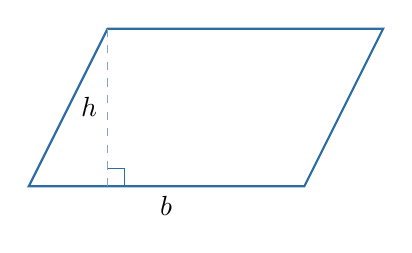
\begin{tikzpicture}
        \draw[thick, color=blu] (0,0) -- (3.5,0) -- (4.5,2) -- (1,2) -- cycle;
        % altezza
        \draw[dashed, color=blu!60] (1,0) -- (1,2);
        \draw[blu] (1,0.22) -- (1.22,0.22) -- (1.22,0);
        \node[below] at (1.75,0) {$b$};
        \node[left]  at (1,1)    {$h$};
    \end{tikzpicture}
\end{center}

\begin{sapevi}
    \textbf{Lo sapevi?} Il parallelogramma è la figura più generale tra quelle studiate in questo capitolo. Rettangolo, rombo e quadrato sono tutti casi particolari di parallelogramma:
    \begin{itemize}[leftmargin=1.5em]
        \item Il \textbf{rettangolo} è un parallelogramma con gli angoli retti.
        \item Il \textbf{rombo} è un parallelogramma con tutti i lati uguali.
        \item Il \textbf{quadrato} è un parallelogramma con gli angoli retti \emph{e} tutti i lati uguali: è quindi sia un rettangolo sia un rombo.
    \end{itemize}
\end{sapevi}

\subsection{Perimetro}

\begin{regola}
    Il \textbf{perimetro del parallelogramma} è la somma dei quattro lati. Poiché i lati opposti sono uguali, si ha:
    \[
        P = 2 \times (b + c)
    \]
    dove $b$ è la base e $c$ è il lato obliquo.
\end{regola}

\begin{esempio}
    Un parallelogramma ha base 11 cm e lato obliquo 5 cm. Calcola il perimetro.

    \medskip
    \textbf{Dati:} $b = 11$ cm, $c = 5$ cm

    \textbf{Formula:} $P = 2 \times (b + c)$

    \textbf{Calcolo:} $P = 2 \times (11 + 5) = 2 \times 16 = 32$ cm

    \textbf{Risposta:} Il perimetro del parallelogramma è \textbf{32 cm}.
\end{esempio}

\subsection{Area}

\begin{regola}
    L'\textbf{area del parallelogramma} si calcola moltiplicando la base per l'altezza corrispondente:
    \[
        A = b \times h
    \]
    dove $b$ è la base e $h$ è l'altezza perpendicolare a quella base.
\end{regola}

\begin{attenzione}
    \textbf{Attenzione:} l'altezza del parallelogramma \emph{non} è il lato obliquo, ma il segmento perpendicolare tra le due basi parallele. Il lato obliquo è sempre più lungo dell'altezza.
\end{attenzione}

\begin{esempio}
    Un parallelogramma ha base 11 cm e altezza 4 cm. Calcola l'area.

    \medskip
    \textbf{Dati:} $b = 11$ cm, $h = 4$ cm

    \textbf{Formula:} $A = b \times h$

    \textbf{Calcolo:} $A = 11 \times 4 = 44$ cm\textsuperscript{2}

    \textbf{Risposta:} L'area del parallelogramma è \textbf{44 cm\textsuperscript{2}}.
\end{esempio}

% =============================================================
\section{Relazioni tra le figure piane}
% =============================================================

Le figure studiate in questo capitolo non sono indipendenti tra loro: alcune sono casi particolari di altre. Lo schema seguente mostra le relazioni di inclusione:

\begin{center}
    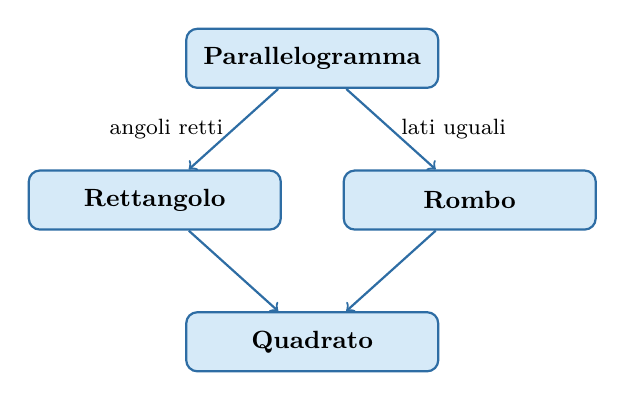
\begin{tikzpicture}[
            box/.style={draw=blu, thick, rounded corners=4pt, fill=azzurro,
                    text=black, font=\small\bfseries,
                    minimum width=3.2cm, minimum height=0.75cm,
                    align=center}
        ]
        % Coordinate assolute: evita la libreria positioning
        \node[box] (par) at (0, 0)    {Parallelogramma};
        \node[box] (ret) at (-2, -1.8) {Rettangolo};
        \node[box] (rom) at ( 2, -1.8) {Rombo};
        \node[box] (qua) at ( 0, -3.6) {Quadrato};

        \draw[thick, color=blu, ->] (par) -- (ret)
        node[midway, left, font=\footnotesize, text=black] {angoli retti};
        \draw[thick, color=blu, ->] (par) -- (rom)
        node[midway, right, font=\footnotesize, text=black] {lati uguali};
        \draw[thick, color=blu, ->] (ret) -- (qua);
        \draw[thick, color=blu, ->] (rom) -- (qua);
    \end{tikzpicture}
\end{center}

\begin{attenzione}
    Il \textbf{trapezio} non è un parallelogramma (ha solo una coppia di lati paralleli, non due). Occupa quindi una categoria separata tra i quadrilateri.
\end{attenzione}

% =============================================================
\section*{Riepilogo del capitolo}
% =============================================================

\begin{regola}
    \textbf{Formule principali — Geometria piana}

    \medskip
    \begin{tabular}{@{}llll@{}}
        \toprule
        \textbf{Figura} & \textbf{Perimetro} & \textbf{Area}                   \\
        \midrule
        Quadrato        & $P = 4l$           & $A = l^2$                       \\[4pt]
        Rettangolo      & $P = 2(b+h)$       & $A = b \times h$                \\[4pt]
        Triangolo       & $P = a+b+c$        & $A = \dfrac{b \times h}{2}$     \\[8pt]
        Trapezio        & $P = B+b+c+d$      & $A = \dfrac{(B+b) \times h}{2}$ \\[8pt]
        Rombo           & $P = 4l$           & $A = \dfrac{d_1 \times d_2}{2}$ \\[8pt]
        Parallelogramma & $P = 2(b+c)$       & $A = b \times h$                \\
        \bottomrule
    \end{tabular}

    \medskip
    \small
    \textit{Legenda:} $l$ = lato; $b$ = base; $h$ = altezza; $a,b,c$ = lati del triangolo;
    $B$ = base maggiore; $c,d$ = lati obliqui; $d_1, d_2$ = diagonali.
\end{regola}

\begin{itemize}[leftmargin=1.5em]
    \item Il \textbf{perimetro} misura il contorno di una figura (unità di lunghezza).
    \item L'\textbf{area} misura la superficie di una figura (unità di superficie).
    \item L'\textbf{altezza} è sempre perpendicolare alla base: non va confusa con un lato obliquo.
    \item Il quadrato è un caso particolare di rettangolo e di rombo; entrambi sono casi particolari di parallelogramma.
    \item Il trapezio ha una sola coppia di lati paralleli: non è un parallelogramma.
\end{itemize}
% ============================================================
%  cap_geometria_solida.tex — Matemagica
%  Geometria solida: cubo e parallelepipedo rettangolo
% ============================================================

\chapter{Geometria solida}

% --- Obiettivi di apprendimento --------------------------------
\section*{Obiettivi di apprendimento}
\begin{itemize}[leftmargin=1.4em]
    \item Comprendere che cosa studia la geometria solida e distinguere i solidi dai piani geometrici.
    \item Riconoscere e descrivere le componenti di un cubo e di un parallelepipedo rettangolo (vertici, spigoli, facce).
    \item Comprendere il concetto di sviluppo piano di un solido.
    \item Calcolare l'area totale e il volume del cubo e del parallelepipedo rettangolo.
    \item Utilizzare correttamente le unità di misura di superficie e di volume.
\end{itemize}

% ============================================================
\section{Che cosa studia la geometria solida}
% ============================================================

Finora abbiamo lavorato con figure geometriche piane: segmenti, angoli, triangoli, quadrilateri. Queste figure esistono su un unico piano e hanno due dimensioni: lunghezza e larghezza.

La \textbf{geometria solida} è il ramo della matematica che studia le figure nello spazio tridimensionale, cioè le figure che hanno tre dimensioni: lunghezza, larghezza e \textbf{altezza} (o profondità). Queste figure sono chiamate \textbf{solidi geometrici}.

\begin{definizione}
    Un \textbf{solido geometrico} è una figura che occupa una porzione limitata dello spazio tridimensionale. A differenza delle figure piane, un solido ha tre dimensioni.
\end{definizione}

I solidi geometrici si dividono in due grandi famiglie:

\begin{itemize}[leftmargin=1.4em]
    \item \textbf{Poliedri}: solidi le cui facce sono tutte superfici piane (poligoni). Esempi: cubo, parallelepipedo, piramide.
    \item \textbf{Solidi di rotazione}: solidi che contengono superfici curve, ottenuti ruotando una figura piana attorno a un asse. Esempi: sfera, cilindro, cono.
\end{itemize}

In questo capitolo ci occuperemo di due poliedri fondamentali: il \textbf{cubo} e il \textbf{parallelepipedo rettangolo}.

% ============================================================
\section{Il volume di un solido}
% ============================================================

\begin{definizione}
    Il \textbf{volume} di un solido è la misura dello spazio che esso occupa.
\end{definizione}

% ============================================================
\section{Il cubo}
% ============================================================

\subsection{Definizione e componenti}

\begin{definizione}
    Il \textbf{cubo} è un solido geometrico poliedrico le cui sei facce sono tutte \textbf{quadrate} e tutte congruenti tra loro. Tutti i suoi spigoli hanno la stessa lunghezza.
\end{definizione}

Il cubo è uno dei solidi più regolari che esistano in geometria. È composto da tre tipi di elementi: \textbf{vertici}, \textbf{spigoli} e \textbf{facce}.

% --- Figura: cubo con etichette ---
\begin{figure}[htb]
    \centering
    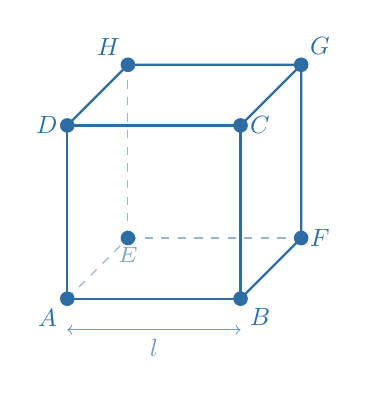
\begin{tikzpicture}[scale=2.2,
            every node/.style={font=\small}]
        % Coordinate dei vertici (cubo unitario in proiezione assonometrica)
        % Faccia anteriore: A B C D, faccia posteriore: E F G H
        \coordinate (A) at (0,0);
        \coordinate (B) at (1,0);
        \coordinate (C) at (1,1);
        \coordinate (D) at (0,1);
        \coordinate (E) at (0.35,0.35);
        \coordinate (F) at (1.35,0.35);
        \coordinate (G) at (1.35,1.35);
        \coordinate (H) at (0.35,1.35);

        % Spigoli nascosti (tratteggiati)
        \draw[dashed, color=blu!50] (A) -- (E);
        \draw[dashed, color=blu!50] (D) -- (H);
        \draw[dashed, color=blu!50] (E) -- (F);
        \draw[dashed, color=blu!50] (E) -- (H);

        % Spigoli visibili
        \draw[thick, color=blu] (A) -- (B) -- (C) -- (D) -- cycle;  % faccia anteriore
        \draw[thick, color=blu] (B) -- (F) -- (G) -- (C);            % faccia destra
        \draw[thick, color=blu] (D) -- (H) -- (G);                   % top e retro
        \draw[thick, color=blu] (F) -- (G) -- (H);                   % faccia superiore destra

        % Vertici
        \foreach \p/\name/\pos in {
                A/A/below left,
                B/B/below right,
                C/C/right,
                D/D/left,
                F/F/right,
                G/G/above right,
                H/H/above left}{
                \fill[blu] (\p) circle (1.2pt);
                \node[\pos, color=blu] at (\p) {$\name$};
            }
        \fill[blu] (E) circle (1.2pt);
        \node[below, color=blu!60] at (E) {\footnotesize$E$};

        % Etichetta lato
        \draw[<->, color=blu!70, thin] (0,-0.18) -- (1,-0.18)
        node[midway, below] {$l$};
    \end{tikzpicture}
    \caption{Il cubo: vertici (A–H), spigoli e facce quadrate.}
\end{figure}

\subsubsection{I vertici}

\begin{definizione}
    I \textbf{vertici} di un solido sono i punti in cui si incontrano gli spigoli. Sono i "angoli" tridimensionali del solido.
\end{definizione}

Il cubo ha \textbf{8 vertici}. Nella figura sono indicati con le lettere A, B, C, D (faccia anteriore) e E, F, G, H (faccia posteriore).

\subsubsection{Gli spigoli}

\begin{definizione}
    Gli \textbf{spigoli} di un solido sono i segmenti in cui si incontrano due facce adiacenti. Sono i "bordi" del solido.
\end{definizione}

Il cubo ha \textbf{12 spigoli}, tutti della stessa lunghezza $l$ (detta \textbf{lato} del cubo).

\subsubsection{Le facce}

\begin{definizione}
    Le \textbf{facce} di un poliedro sono i poligoni piani che delimitano il solido. Ogni faccia è una superficie piana.
\end{definizione}

Il cubo ha \textbf{6 facce}, tutte quadrate con lato $l$. Le sei facce sono disposte a \textbf{coppie su piani paralleli}:
\begin{itemize}[leftmargin=1.4em]
    \item faccia anteriore e faccia posteriore (parallele tra loro);
    \item faccia superiore e faccia inferiore (parallele tra loro);
    \item faccia destra e faccia sinistra (parallele tra loro).
\end{itemize}

\begin{sapevi}
    \textbf{Lo sapevi?} Il cubo prende il nome dalla parola greca \emph{kybos}, che significa "dado". I dadi a sei facce usati nei giochi hanno esattamente la forma di un cubo! In matematica il cubo è anche chiamato \textbf{esaedro regolare}, perché ha 6 facce regolari uguali. È uno dei soli cinque solidi completamente regolari, noti come \emph{solidi platonici}.
\end{sapevi}

% ============================================================
\subsection{Lo sviluppo piano del cubo}
% ============================================================

\begin{definizione}
    Lo \textbf{sviluppo piano} (o \textbf{netto}) di un solido è la figura piana che si ottiene aprendo e distendendo tutte le facce del solido su un piano, come se si aprissero le pieghe di una scatola.
\end{definizione}

Lo sviluppo piano è utile per due motivi: permette di visualizzare tutte le facce del solido contemporaneamente, e consente di calcolare l'\textbf{area totale} del solido.

Il cubo ha molti sviluppi piani possibili (11 in totale); il più semplice è a forma di croce:

% --- Figura: sviluppo piano del cubo ---
\begin{figure}[htb]
    \centering
    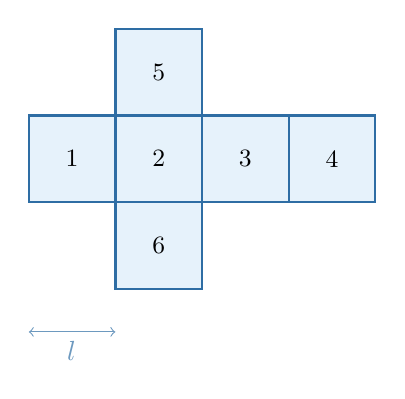
\begin{tikzpicture}[scale=1.0]
        \def\s{1.1} % lato quadrato
        % Riga centrale: 4 quadrati (sx, centro-sx, centro-dx, dx)
        \foreach \i in {0,1,2,3} {
                \draw[thick, color=blu, fill=azzurro!60]
                (\i*\s, 0) rectangle (\i*\s+\s, \s);
            }
        % Sopra la seconda casella
        \draw[thick, color=blu, fill=azzurro!60]
        (\s, \s) rectangle (2*\s, 2*\s);
        % Sotto la seconda casella
        \draw[thick, color=blu, fill=azzurro!60]
        (\s, -\s) rectangle (2*\s, 0);
        % Etichette facce
        \node at (0.5*\s, 0.5*\s) {\small 1};
        \node at (1.5*\s, 0.5*\s) {\small 2};
        \node at (2.5*\s, 0.5*\s) {\small 3};
        \node at (3.5*\s, 0.5*\s) {\small 4};
        \node at (1.5*\s, 1.5*\s) {\small 5};
        \node at (1.5*\s, -0.5*\s) {\small 6};
        % Etichetta lato
        \draw[<->, thin, color=blu!70] (0, -1.5*\s) -- (\s, -1.5*\s)
        node[midway, below] {$l$};
    \end{tikzpicture}
    \caption{Uno sviluppo piano del cubo (le 6 facce quadrate numerate da 1 a 6).}
\end{figure}

\begin{attenzione}
    \textbf{Attenzione.} Non tutti i modi di disporre 6 quadrati uniti per un lato sono sviluppi validi del cubo. Esistono esattamente \textbf{11} disposizioni diverse che, una volta ripiegate, formano un cubo corretto.
\end{attenzione}

% ============================================================
\subsection{Area totale del cubo}
% ============================================================

\begin{definizione}
    L'\textbf{area totale} di un solido è la somma delle aree di tutte le sue facce. Rappresenta la superficie complessiva del solido.
\end{definizione}

Poiché il cubo ha 6 facce quadrate tutte uguali, ciascuna con lato $l$, l'area di ciascuna faccia è $l^2$. Quindi:

\begin{regola}
    \textbf{Area totale del cubo}

    Dato un cubo di lato $l$:
    \[
        A_{\text{tot}} = 6 \cdot l^2
    \]
    L'area totale si misura in unità quadrate (cm², m², …).
\end{regola}

\begin{esempio}
    \textbf{Calcolo dell'area totale di un cubo.}

    Un cubo ha lato $l = 4\,\text{cm}$. Calcola la sua area totale.

    \medskip
    \textit{Soluzione:}
    \[
        A_{\text{tot}} = 6 \cdot l^2 = 6 \cdot 4^2 = 6 \cdot 16 = 96\,\text{cm}^2
    \]

    L'area totale del cubo è $96\,\text{cm}^2$.
\end{esempio}

% ============================================================
\subsection{Volume del cubo}
% ============================================================

\begin{regola}
    \textbf{Volume del cubo}

    Dato un cubo di lato $l$:
    \[
        V = l^3
    \]

    Si legge: "$l$ al cubo". Non a caso, la terza potenza di un numero si chiama proprio \textbf{cubo} in riferimento a questo solido.
\end{regola}

\begin{esempio}
    \textbf{Calcolo del volume di un cubo.}

    Un cubo ha lato $l = 3\,\text{dm}$. Calcola il suo volume.

    \medskip
    \textit{Soluzione:}
    \[
        V = l^3 = 3^3 = 27\,\text{dm}^3
    \]

    Il volume del cubo è $27\,\text{dm}^3$.
\end{esempio}

\begin{attenzione}
    \textbf{Errore comune.} Molti studenti confondono area totale e volume, oppure dimenticano l'esponente corretto. Ricorda:
    \begin{itemize}[leftmargin=1.4em]
        \item Area totale del cubo: $A = 6l^{\mathbf{2}}$ \quad (esponente 2, unità quadrate)
        \item Volume del cubo: $V = l^{\mathbf{3}}$ \quad (esponente 3, unità cubiche)
    \end{itemize}
\end{attenzione}

% ============================================================
\section{Il parallelepipedo rettangolo}
% ============================================================

\subsection{Definizione e componenti}

\begin{definizione}
    Il \textbf{parallelepipedo rettangolo} è un solido geometrico \textbf{poliedrico} le cui 6 facce sono tutte rettangolari. Le facce opposte sono \textbf{congruenti} (hanno la stessa forma e le stesse dimensioni) e giacciono su piani paralleli.
\end{definizione}

\medskip
\textbf{Perché si chiama "rettangolo"?} Il termine "rettangolo" indica che tutti gli angoli tra le facce (detti \textbf{angoli diedri}) sono angoli retti, cioè di $90°$. Esistono anche parallelepipedi \emph{obliqui}, in cui le facce laterali non sono perpendicolari alla base; nel programma di scuola media si studia però solo il parallelepipedo rettangolo.

\medskip
\textbf{Che cosa significa "poliedrico"?} Un solido si dice \textbf{poliedrico} (o \textbf{poliedro}) quando tutte le sue facce sono poligoni piani. Il termine viene dal greco \emph{polys} (molti) e \emph{hedra} (facce). Il cubo e il parallelepipedo rettangolo sono entrambi poliedri.

% --- Figura: parallelepipedo rettangolo ---
\begin{figure}[htb]
    \centering
    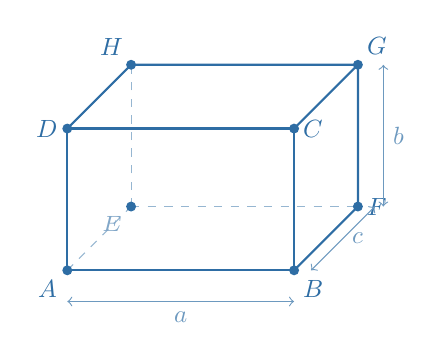
\begin{tikzpicture}[scale=1.8,
            every node/.style={font=\small}]
        % Dimensioni: a=1.6, b=1, c=0.55 (proiezione)
        \def\a{1.6} \def\b{1.0} \def\offs{0.45}

        \coordinate (A) at (0,0);
        \coordinate (B) at (\a,0);
        \coordinate (C) at (\a,\b);
        \coordinate (D) at (0,\b);
        \coordinate (E) at (\offs,\offs);
        \coordinate (F) at (\a+\offs,\offs);
        \coordinate (G) at (\a+\offs,\b+\offs);
        \coordinate (H) at (\offs,\b+\offs);

        % Spigoli nascosti
        \draw[dashed, color=blu!50] (A) -- (E);
        \draw[dashed, color=blu!50] (D) -- (H);
        \draw[dashed, color=blu!50] (E) -- (F);
        \draw[dashed, color=blu!50] (E) -- (H);

        % Spigoli visibili
        \draw[thick, color=blu] (A) -- (B) -- (C) -- (D) -- cycle;
        \draw[thick, color=blu] (B) -- (F) -- (G) -- (C);
        \draw[thick, color=blu] (D) -- (H) -- (G);
        \draw[thick, color=blu] (F) -- (G) -- (H);

        % Vertici
        \foreach \p/\name/\pos in {
                A/A/below left, B/B/below right, C/C/right,
                D/D/left, F/F/right, G/G/above right, H/H/above left}{
                \fill[blu] (\p) circle (1pt);
                \node[\pos, color=blu] at (\p) {$\name$};
            }
        \fill[blu] (E) circle (1pt);
        \node[below left, color=blu!60, font=\footnotesize] at (E) {$E$};

        % Quote dimensioni
        \draw[<->, thin, color=blu!70] (0,-0.22) -- (\a,-0.22)
        node[midway, below] {$a$};
        \draw[<->, thin, color=blu!70] (\a+\offs+0.18, \offs) -- (\a+\offs+0.18, \b+\offs)
        node[midway, right] {$b$};
        \draw[<->, thin, color=blu!70] (\a+0.12, 0) -- (\a+\offs+0.12, \offs)
        node[midway, right] {$c$};
    \end{tikzpicture}
    \caption{Il parallelepipedo rettangolo con dimensioni $a$ (lunghezza), $b$ (altezza), $c$ (larghezza/profondità).}
\end{figure}

Il parallelepipedo rettangolo ha tre dimensioni distinte:
\begin{itemize}[leftmargin=1.4em]
    \item $a$ = \textbf{lunghezza} (o base);
    \item $b$ = \textbf{altezza};
    \item $c$ = \textbf{larghezza} (o profondità).
\end{itemize}

\subsubsection{I vertici}
Il parallelepipedo rettangolo ha \textbf{8 vertici} (A, B, C, D nella faccia anteriore; E, F, G, H nella faccia posteriore), esattamente come il cubo.

\subsubsection{Gli spigoli}
Il parallelepipedo rettangolo ha \textbf{12 spigoli}, divisi in tre gruppi di 4 spigoli paralleli e congruenti tra loro:
\begin{itemize}[leftmargin=1.4em]
    \item 4 spigoli di lunghezza $a$;
    \item 4 spigoli di lunghezza $b$;
    \item 4 spigoli di lunghezza $c$.
\end{itemize}

\subsubsection{Le facce}
Il parallelepipedo rettangolo ha \textbf{6 facce rettangolari}, disposte a \textbf{coppie congruenti} su piani paralleli:

\begin{itemize}[leftmargin=1.4em]
    \item 2 facce di dimensioni $a \times b$ (faccia anteriore e posteriore);
    \item 2 facce di dimensioni $b \times c$ (faccia destra e sinistra);
    \item 2 facce di dimensioni $a \times c$ (faccia superiore e inferiore).
\end{itemize}

\medskip
\textbf{Che cosa significa "congruente"?} Due figure geometriche sono \textbf{congruenti} quando hanno esattamente la stessa forma e le stesse dimensioni: sovrapposte perfettamente, coincidono punto per punto. In geometria solida si usa anche il termine tecnico \textbf{isometrico} (dal greco \emph{isos} = uguale, \emph{metron} = misura), che ha lo stesso significato. Nel linguaggio scolastico si preferisce "congruente".

\begin{attenzione}
    \textbf{Cubo o parallelepipedo?} Il cubo è un caso \emph{particolare} di parallelepipedo rettangolo, in cui le tre dimensioni sono tutte uguali: $a = b = c = l$. Ogni cubo è quindi un parallelepipedo rettangolo, ma non ogni parallelepipedo rettangolo è un cubo.
\end{attenzione}

% ============================================================
\subsection{Lo sviluppo piano del parallelepipedo rettangolo}
% ============================================================

Come per il cubo, è possibile "aprire" il parallelepipedo rettangolo e distendere tutte le facce su un piano per ottenere il suo \textbf{sviluppo piano}.

% --- Figura: sviluppo piano del parallelepipedo ---
\begin{figure}[htb]
    \centering
    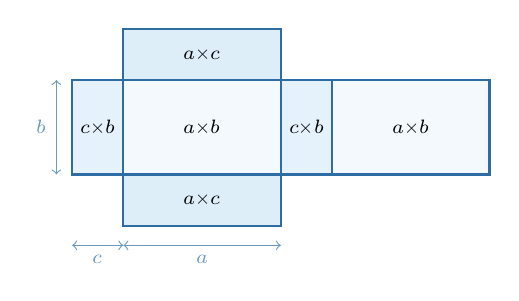
\begin{tikzpicture}[scale=1.0]
        \def\a{2.0}  % lunghezza
        \def\b{1.2}  % altezza
        \def\c{0.65} % larghezza/profondità

        % Riga centrale: c | a | c | a
        % y=0 è la linea inferiore della riga centrale
        % Faccia c×b (sinistra)
        \draw[thick, color=blu, fill=azzurro!60]
        (0,0) rectangle (\c,\b);
        \node[font=\scriptsize] at (0.5*\c, 0.5*\b) {$c{\times}b$};

        % Faccia a×b (centro-sinistra)
        \draw[thick, color=blu, fill=azzurro!30]
        (\c,0) rectangle (\c+\a,\b);
        \node[font=\scriptsize] at (\c+0.5*\a, 0.5*\b) {$a{\times}b$};

        % Faccia c×b (centro-destra)
        \draw[thick, color=blu, fill=azzurro!60]
        (\c+\a,0) rectangle (2*\c+\a,\b);
        \node[font=\scriptsize] at (\c+\a+0.5*\c, 0.5*\b) {$c{\times}b$};

        % Faccia a×b (destra)
        \draw[thick, color=blu, fill=azzurro!30]
        (2*\c+\a,0) rectangle (2*\c+2*\a,\b);
        \node[font=\scriptsize] at (2*\c+\a+0.5*\a, 0.5*\b) {$a{\times}b$};

        % Faccia a×c (sopra)
        \draw[thick, color=blu, fill=azzurro!80]
        (\c,\b) rectangle (\c+\a,\b+\c);
        \node[font=\scriptsize] at (\c+0.5*\a, \b+0.5*\c) {$a{\times}c$};

        % Faccia a×c (sotto)
        \draw[thick, color=blu, fill=azzurro!80]
        (\c,-\c) rectangle (\c+\a,0);
        \node[font=\scriptsize] at (\c+0.5*\a, -0.5*\c) {$a{\times}c$};

        % Quote
        \draw[<->, thin, color=blu!70] (\c, -\c-0.25) -- (\c+\a, -\c-0.25)
        node[midway, below, font=\scriptsize] {$a$};
        \draw[<->, thin, color=blu!70] (-0.2, 0) -- (-0.2, \b)
        node[midway, left, font=\scriptsize] {$b$};
        \draw[<->, thin, color=blu!70] (0, -\c-0.25) -- (\c, -\c-0.25)
        node[midway, below, font=\scriptsize] {$c$};
    \end{tikzpicture}
    \caption{Uno sviluppo piano del parallelepipedo rettangolo con dimensioni $a$, $b$, $c$.}
\end{figure}

% ============================================================
\subsection{Area totale del parallelepipedo rettangolo}
% ============================================================

Dallo sviluppo piano si vede chiaramente che l'area totale è la somma delle aree delle 3 coppie di facce congruenti:

\begin{regola}
    \textbf{Area totale del parallelepipedo rettangolo}

    Dato un parallelepipedo rettangolo con dimensioni $a$, $b$, $c$:
    \[
        A_{\text{tot}} = 2\,(ab + bc + ca)
    \]
    dove:
    \begin{itemize}[leftmargin=1.4em, nosep]
        \item $ab$ è l'area della coppia di facce anteriore/posteriore;
        \item $bc$ è l'area della coppia di facce destra/sinistra;
        \item $ca$ è l'area della coppia di facce superiore/inferiore.
    \end{itemize}
\end{regola}

\begin{esempio}
    \textbf{Calcolo dell'area totale di un parallelepipedo rettangolo.}

    Un parallelepipedo rettangolo ha dimensioni $a = 5\,\text{cm}$, $b = 3\,\text{cm}$, $c = 2\,\text{cm}$. Calcola la sua area totale.

    \medskip
    \textit{Soluzione:}
    \begin{align*}
        ab             & = 5 \cdot 3 = 15\,\text{cm}^2                     \\
        bc             & = 3 \cdot 2 = 6\,\text{cm}^2                      \\
        ca             & = 2 \cdot 5 = 10\,\text{cm}^2                     \\[4pt]
        A_{\text{tot}} & = 2\,(15 + 6 + 10) = 2 \cdot 31 = 62\,\text{cm}^2
    \end{align*}

    L'area totale è $62\,\text{cm}^2$.
\end{esempio}

% ============================================================
\subsection{Volume del parallelepipedo rettangolo}
% ============================================================

\begin{regola}
    \textbf{Volume del parallelepipedo rettangolo}

    Dato un parallelepipedo rettangolo con dimensioni $a$, $b$, $c$:
    \[
        V = a \cdot b \cdot c
    \]

    \medskip
    \textit{Nota:} Se $a = b = c = l$, si ottiene la formula del cubo: $V = l \cdot l \cdot l = l^3$.
\end{regola}

\begin{esempio}
    \textbf{Calcolo del volume di un parallelepipedo rettangolo.}

    Una scatola ha lunghezza $a = 20\,\text{cm}$, larghezza $c = 15\,\text{cm}$ e altezza $b = 10\,\text{cm}$. Calcola il suo volume.

    \medskip
    \textit{Soluzione:}
    \[
        V = a \cdot b \cdot c = 20 \cdot 10 \cdot 15 = 3\,000\,\text{cm}^3
    \]

    Il volume della scatola è $3\,000\,\text{cm}^3$.
\end{esempio}

\begin{attenzione}
    \textbf{Errore comune.} Per calcolare il volume si moltiplicano le \emph{tre} dimensioni, non due. Moltiplicare solo $a \cdot b$ dà l'area di una faccia, non il volume.

    \medskip
    Verifica sempre che le tre misure siano espresse nella \emph{stessa} unità prima di calcolare: se una dimensione è in cm e un'altra in m, converti prima di moltiplicare.
\end{attenzione}

\begin{sapevi}
    \textbf{Lo sapevi?} Il parallelepipedo rettangolo è la forma di moltissimi oggetti della vita quotidiana: mattoni, scatole, libri, stanze. Quando architetti e ingegneri calcolano quanta vernice serve per tinteggiare una stanza, usano esattamente la formula dell'area totale del parallelepipedo. Il volume è invece la grandezza chiave per sapere quanta aria contiene una stanza o quanta acqua entra in una vasca.
\end{sapevi}

% ============================================================
\section{Riepilogo del capitolo}
% ============================================================

\begin{tcolorbox}[
        enhanced, breakable,
        colback  = azzurro,
        colframe = blu,
        fonttitle = \bfseries,
        title    = {Riepilogo — Geometria solida},
    ]

    \textbf{Geometria solida:} studia le figure nello spazio tridimensionale.

    \medskip
    \textbf{Poliedro:} solido le cui facce sono tutte poligoni piani. Cubo e parallelepipedo rettangolo sono poliedri.

    \medskip
    \textbf{Vertici, spigoli, facce:}
    \begin{itemize}[leftmargin=1.4em, nosep]
        \item \emph{Vertice}: punto in cui si incontrano gli spigoli.
        \item \emph{Spigolo}: segmento in cui si incontrano due facce.
        \item \emph{Faccia}: poligono piano che delimita il solido.
    \end{itemize}

    \medskip
    \textbf{Cubo} (lato $l$): 8 vertici, 12 spigoli, 6 facce quadrate.
    \[
        A_{\text{tot}} = 6l^2 \qquad V = l^3
    \]

    \textbf{Parallelepipedo rettangolo} (dimensioni $a,b,c$): 8 vertici, 12 spigoli, 6 facce rettangolari a coppie congruenti.
    \[
        A_{\text{tot}} = 2(ab+bc+ca) \qquad V = a \cdot b \cdot c
    \]

    \medskip
    \textbf{Sviluppo piano:} figura piana ottenuta aprendo tutte le facce del solido su un piano.

\end{tcolorbox}


% =============================================================
\end{document}
% =============================================================
